%%*********************************************************
%% Essa versão corresponde ao padrão CCPG 001/2015.
%%
%% Ela foi adaptada do trabalho anterior de várias pessoas,
%% e mais detalhes podem ser encontrados abaixo.
%% 
%% Adriano Batista Prieto, 16 de outubro de 2015.
%% adrianoprieto@yahoo.com.br
%% *********************************************************
%Modelos para a edição de dissertações e teses
%
%Modelo LaTeX segundo o formato especificado na Informação CCPG 002/2013.
% http://www.prpg.unicamp.br/arqpdfnormas/infccpg002_2013.pdf
%
%Esse modelo para a edição de dissertações e teses foi adaptado da versão elaborada pelos alunos Daniel Guerreiro e Silva, Filipe Ieda Fazanaro e  Marcos Ricardo Covre da Faculdade de Engenharia Elétrica e de Computação
%
%http://www0.fee.unicamp.br/cpg/Modelos.html
%
%Modelo baseado no abntex2 disponível em https://code.google.com/p/abntex2/
%
%Instruções para instalação do abntex2 disponíveis em https://code.google.com/p/abntex2/wiki/Instalacao
%
%
%%
%% Faculdade de Tecnologia - Junho/2014.
% ------------------------------------------------------------------------

%ARQUIVO DE PREAMBULO DA TESE - PACOTES E CONFIGURAÇÕES

\documentclass[
	% -- opções da classe memoir --
	12pt,				% tamanho da fonte
	openright,			% capítulos começam em pág ímpar (insere página vazia caso preciso)
	oneside,			% para impressão em verso e verso use twoside.
	a4paper,		% tamanho do papel. ... letterpaper
	% -- opções da classe abntex2 --
	%chapter=TITLE,		% títulos de capítulos convertidos em letras maiúsculas
	%section=TITLE,		% títulos de seções convertidos em letras maiúsculas
	%subsection=TITLE,	% títulos de subseções convertidos em letras maiúsculas
	%subsubsection=TITLE,% títulos de subsubseções convertidos em letras maiúsculas
	% -- opções do pacote babel --
	english,			% idioma adicional para hifenização
	%french,			% idioma adicional para hifenização
	%spanish,			% idioma adicional para hifenização
	brazil,				% o último idioma é o principal do documento
	sumario=tradicional,
	]{abntex2}

% ---
% Pacotes fundamentais
% ---
\usepackage{cmap}				% Mapear caracteres especiais no PDF
\usepackage{lmodern}			% Usa a fonte Latin Modern		
\usepackage[T1]{fontenc}		% Selecao de codigos de fonte.
%\usepackage[latin1]{inputenc}	% Codificacao do documento (conversão automática dos acentos)
\usepackage[utf8]{inputenc}		% Codificacao do documento (conversão automática dos acentos)
\usepackage{lastpage}			% Usado pela Ficha catalográfica
\usepackage{indentfirst}		% Indenta o primeiro parágrafo de cada seção.
\usepackage{color}				% Controle das cores
\usepackage[pdftex]{graphicx}	% Inclusão de gráficos
\usepackage{epstopdf}           % Pacote que converte as figuras em eps para pdf
\usepackage{lscape} % páginas na horizontal.
\usepackage{scalefnt} % pra reduzir o tamanho de fontes 
% ---
		
% ---
% Pacotes adicionais, usados apenas no âmbito do Modelo Canônico do abnteX2
% ---
\usepackage{nomencl}
\usepackage{amsmath}
\usepackage{bbm}
\usepackage[chapter]{algorithm}
\usepackage{algorithmic}
\usepackage{multirow}
\usepackage{rotating}
\usepackage{pdfpages}
% ---

% ---
% Pacotes de citações
% ---
%\usepackage[brazilian,hyperpageref]{backref}	 % Paginas com as citações na bibl
\usepackage[alf,abnt-etal-cite=2,abnt-etal-list=0,abnt-etal-text=emph]{abntex2cite}	% Citações padrão ABNT

% ---
% Pacote de customização - Unicamp
% ---
\usepackage{unicamp}


% ---
% CONFIGURAçõES DE PACOTES
% ---

% ---
% Configurações do pacote backref
% Usado sem a opção hyperpageref de backref

%customização do negrito em ambientes matemáticos
\newcommand{\mb}[1]{\mathbf{#1}}
%customização de teoremas
\newtheorem{mydef}{Definição}[chapter]
\newtheorem{lemm}{Lema}[chapter]
\newtheorem{theorem}{Teorema}[chapter]
\floatname{algorithm}{Pseudoc\'{o}digo}
\renewcommand{\listalgorithmname}{Lista de Pseudoc\'{o}digos}

% Para mudar fonte dos títulos de capítulos, de secões, etc  para padrão Latex (fonte cmr) descomente a linha a seguir. 

%\renewcommand{\ABNTEXchapterfont}{\fontfamily{cmr}\fontseries{b}\selectfont}

% ---
% Configurações de aparência do PDF final

% alterando o aspecto da cor azul
\definecolor{blue}{RGB}{41,5,195}

% informações do PDF
\makeatletter
\hypersetup{
     	%pagebackref=true,
		pdftitle={\@title},
		pdfauthor={\@author},
    	pdfsubject={\imprimirpreambulo},
	    pdfcreator={LaTeX with abnTeX2},
		pdfkeywords={abnt}{latex}{abntex}{abntex2}{trabalho acad\^{e}mico},
		%hidelinks,					% desabilita as bordas dos links
		colorlinks=true,       	    % false: boxed links; true: colored links
		% aqui vc pode trocar a cor dos links do sumário, lista de figs, etc.
    	linkcolor=red,          	% color of internal links
    	citecolor=blue,        		% color of links to bibliography
    	filecolor=magenta,      	% color of file links
		urlcolor=blue,
%		linkbordercolor={1 1 1},	% set to white
		bookmarksdepth=4
}
\makeatother
% ---

% ---
% Espaçamentos entre linhas e parágrafos
% ---

% O tamanho do parágrafo é dado por:
\setlength{\parindent}{2.0cm}

% Controle do espaçamento entre um parágrafo e outro:
\setlength{\parskip}{0.2cm}  % tente também \onelineskip

% ---
% Informacoes de dados para CAPA e FOLHA DE ROSTO
% ---
\titulo{Autovalores com Algoritmos Genéticos}
\autor{Adriano Batista Prieto}
\local{Limeira}
\data{2015}
\orientador{Prof. Dr. Vitor Rafael Coluci}
%\coorientador[Co-orientador]{Prof. Dr. Co-orientador}
\instituicao{%
    UNIVERSIDADE ESTADUAL DE CAMPINAS
    \par
    Faculdade de Tecnologia
    }
%\tipotrabalho{Tese (Doutorado)}
%\preambulo{Tese apresentada à Faculdade de Tecnologia da Universidade Estadual de Campinas como parte dos requisitos exigidos para a obtenção do título de Doutor em Tecnologia, na área de Ciências dos Materiais, Sistemas de Informação e Comunicação ou Ambiente.}
\tipotrabalho{Dissertação (Mestrado)}
\preambulo{Dissertação apresentada à Faculdade de Tecnologia da Universidade Estadual de Campinas como parte dos requisitos exigidos para a obtenção do título de Mestre em Tecnologia, na área de Tecnologia e Inovação.}
% --- 


% ---- compila o índice  ----
\makeindex
\makenomenclature
% ---

% ---- Início do documento ----
\begin{document}

% Retira espaço extra obsoleto entre as frases.
\frenchspacing

% ---- ELEMENTOS PRÉ-TEXTUAIS ----
\pretextual

%\pagenumbering{roman}

% 1. Capa
\imprimircapa
% ---

% 2. Folha de Rosto. (o * indica que haverá a ficha catalográfica) ---
\thispagestyle{empty}
\imprimirfolhaderosto*
% --

% 3. Ficha catalográfica ---

% A biblioteca da FT lhe fornecerá um PDF
% com a ficha catalográfica definitiva após a defesa do trabalho. Quando estiver
% com o documento, salve-o como PDF no diretório do seu projeto e substitua todo
% o conteúdo de implementação deste arquivo pelo comando abaixo:

% --- Para a versão final, delete as linhas abaixo e insira a linha do \includepdf
\thispagestyle{empty}
 \begin{fichacatalografica}
    \vspace*{\fill}
    \begin{center}
        \textsc{Inclua aqui o pdf com a ficha catalográfica fornecida.}
    \end{center}
    \vspace*{\fill}
% --- --- ---
    %\includepdf{./figs/ficha-catalografica.pdf}
 \end{fichacatalografica}
% ---


% 4. Folha de aprovação ---

% Após a aprovação do trabalho, substitua todo o conteúdo deste arquivo por uma
% imagem da página assinada pela banca com o comando abaixo:

% --- Na versão final, exclua essas linhas e insira o \includepdf
\newpage
\thispagestyle{empty}
\vspace*{\fill}
\begin{center}
    \textsc{Inclua aqui a Folha de aprovação.}
\end{center}
\vspace*{\fill}
\newpage
% --- --- ---
%\includepdf[pagecommand={\thispagestyle{plain}}]{./figs/folha-assinaturas.pdf}	
\cleardoublepage

% 5. Dedicatória ---
\begin{dedicatoria}
    \thispagestyle{empty}
		\vspace*{\fill}
    \centering
    \noindent
    \textit{Dedico esta tese à todo mundo.}
    \vspace*{\fill}
\end{dedicatoria}
% ---

% 6. Agradecimentos ---
\begin{agradecimentos}
    \thispagestyle{empty}
    Agradecimentos aqui.
\end{agradecimentos}

% ---

% --- Epígrafe  ---
\begin{epigrafe}
	\thispagestyle{empty}
    \vspace*{\fill}
	\begin{flushright}
		\textit{``Escreva aqui a sua epígrafe''\\
		(Citação)}
	\end{flushright}
\end{epigrafe}


\thispagestyle{empty}
\begin{resumo}
			% 7. RESUMO em português
     Colocar o resumos aqui.
     
    \vspace{\onelineskip}

    \noindent\textbf{Palavras-chaves}: palavra-chave 1; palavra-chave 2; palavra-chave 3.

    \vspace{\onelineskip}
    \vspace{\onelineskip}
		
		% 8. Abstract (resumo traduzido para o inglês);
    \begin{otherlanguage*}{english}
    \begin{center}{\ABNTEXchapterfont\huge Abstract}\end{center}
    
    Put abstract here.
    \vspace{\onelineskip}

    \noindent\textbf{Keywords}: keyword 1; keyword 2; keyword 3.

    \end{otherlanguage*}
		
		% 9. Resumo em uma terceira língua (opcional);
		% \begin{otherlanguage*}{english} %% substitua o ``english'' pelo idioma desejado.
    % \begin{center}{\ABNTEXchapterfont\huge Abstract}\end{center}
    
    % Put abstract here.
    % \vspace{\onelineskip}

    % \noindent\textbf{Keywords}: keyword 1; keyword 2; keyword 3.

    % \end{otherlanguage*}
		
\end{resumo}

% 10. Lista de ilustrações (opcional);
\pdfbookmark[0]{\listfigurename}{lof}
\listoffigures*
\thispagestyle{empty}
\cleardoublepage
% ---

% 11. Lista de Tabelas (opcional);
\pdfbookmark[0]{\listtablename}{lot}
\listoftables*
\thispagestyle{empty}
\cleardoublepage
% ---

% 12. Lista de Abreviaturas e Siglas (opcional);
\renewcommand{\nomname}{Lista de Acrônimos e Abreviações}
\pdfbookmark[0]{\nomname}{las}
\printnomenclature
\thispagestyle{empty}
\cleardoublepage
% ---

% 13. Lista de Símbolos (opcional);

% ---

% 14. Sumário.
\pdfbookmark[0]{\contentsname}{toc}
\tableofcontents*
\thispagestyle{empty}
\cleardoublepage
% ---

% ---- ELEMENTOS TEXTUAIS ----
\textual

% ---- Capítulos ----
\chapter{Introdução}
\label{cap:introducao}

\setcounter{page}{12}

	O problema dos autovalores e autovetores pode ser definido brevemente da seguinte maneira: dada uma matriz $\mathsf{A}$ $n$ por $n$, o escalar $\lambda$ é chamado de \textbf{autovalor} de $\mathsf{A}$ se existe um vetor \textbf{\texttt{u}} não nulo tal que

\begin{equation}\label{eq:autovalor_intro}
	\mathsf{A} \textbf{\texttt{u}} = \lambda \textbf{\texttt{u}}.
\end{equation}

O vetor \textbf{\texttt{u}} é chamado de \textbf{autovetor} de $\mathsf{A}$ associado a $\lambda$. Reescrevendo a equação \ref{eq:autovalor_intro} chegamos a 

\begin{equation}
		\begin{array}{c}
			\mathsf{A} \textbf{\texttt{u}} - \lambda \textbf{\texttt{u}} = 0 \\
			(\mathsf{A} - \lambda \mathsf{I})\textbf{\texttt{u}} = 0,
		\end{array}
\end{equation}
onde $\mathsf{I}$ é a matriz identidade. Pela teoria das equações lineares, a equação acima só tem soluções se

\begin{equation}\label{eq:detIntro}
	\mbox{det}(\mathsf{A} - \lambda \mathsf{I}) = 0.
\end{equation}

A equação \ref{eq:detIntro} é chamada de \textbf{Equação Característica} de $\mathsf{A}$, e leva a um \textbf{Polinômio Característico} de ordem $n$. Portanto, $\mathsf{A}$ pode ter até $n$ autovalores.

	Mas, de onde vieram os autovalores? O que são? Por que são importantes? Muitos estudantes de ciências exatas e engenharia fazem essas três perguntas durante as disciplinas introdutórias de Álgebra Linear. Uma descrição mais detalhada da importância histórica dos autovalores, além dos métodos numéricos clássicos, pode ser encontrada no Apêndice \ref{apdx:historia}.
	
	A primeira aparição dos autovalores aconteceu no século $\mathsf{XVII}$. A partir de então grandes nomes da matemática se debruçaram sobre o estudo da sua natureza, como D'Alembert, Lagrange, Laplace, Sturm e Cauchy, culminando no final do século $\mathsf{XIX}$ na Teoria Espectral das Matrizes. No início do século $\mathsf{XX}$ os autovalores foram fundamentais dentro da Mecânica Quântica, uma das grandes revoluções científicas e culturais da nossa era. Com o advento do computador eletrônico por volta de 1950, a criação de métodos numéricos tornou-se muito ativa \cite{Hawkins75}.
	
	No século $\mathsf{XXI}$ a relevância continua. A busca pela palavra \emph{eigenvalue} em periódicos como \emph{Nature} e \emph{Science} revela os autovalores continuam muito utilizados. Google, Facebook e Twitter, por exemplo, estão fortemente relacionados aos autovalores. Dado o número de usuários desses sistemas, no mínimo da ordem de centenas de milhões \cite{twitter2010}, passou-se a buscar métodos com alto potencial para uso de algoritmos paralelos e computação de alto desempenho.
	
	Apresento nessa dissertação o estudo de um método com esse potencial. Em uma série de artigos, com \cite{metodo2004} sendo o primeiro, é proposta uma maneira de encontrar o autovalor mínimo de uma matriz simétrica. Para isso fazem uso de Algoritmos Genéticos \cite{Mitchell98}, que são intrinsecamente paralelos \cite{Linden2008} e, dependendo do problema modelado e da arquitetura de computação paralela escolhida, altamente escaláveis. Essas características já foram exploradas de maneira sistemática em arquiteturas tradicionais \cite{Cantu-Paz2000}, e mais recentemente bons desempenhos foram atingidos com GAs simples executados em placas de vídeo (GPUs) com arquitetura NVIDIA CUDA. Em \cite{onemaxNaGPU} o GA paralelizado na GPU chegou a ser até trinta vezes mais rápido.

	Assim, inicialmente os principais objetivos para o projeto foram:
	
	\begin{enumerate}
		\item Desenvolver um programa serial que implementasse o método apresentado em \cite{metodo2004};
		
		\item Reproduzir os resultados de \cite{metodo2004};
		
		\item Desenvolver uma versão paralela do programa na arquitetura NVIDIA CUDA;
		
		\item Comparar o desempenho do programa Serial com o programa Paralelo.
	\end{enumerate}
	
	A \textbf{hipótese} era que o programa paralelo seria mais rápido, e o objetivo era quantificar esse ganho. Porém, a pesquisa tomou outro rumo.
	
	Encontrei uma falha em \cite{metodo2004}. O artigo afirma que o método obtém sempre o autovalor mínimo de matrizes simétricas. Com base em resultados experimentais próprios, em conhecidas propriedades do Quociente de Rayleigh e em um erro, argumento que não há garantias de se encontrar o menor autovalor. É possível que os autores tenham omitido algum procedimento específico.
	
	Dos cinco artigos que utilizam o método, o último \cite{metodo2011} possui uma diferença significativa: a Função de Avaliação (\emph{fitness}) do Algoritmo Genético foi alterada. Essa função tem papel fundamental em todo algoritmo genético, pois é a maneira utilizada pelos GAs para determinar a qualidade de um indivíduo como solução do problema \cite{Linden2008}. Isso me motivou a estudar \cite{metodo2011} em detalhes, e identifiquei que, justamente por causa do novo \emph{fitness}, o erro lógico dos trabalhos anteriores não foi cometido.
	
	Dado o contexto, surgiram duas novas hipóteses:
	
	\textbf{Hipótese 1}: a impossibilidade de se obter o menor autovalor com \cite{metodo2004} não reside em uma falha do método, mas apenas na má definição da Função de Avaliação.
	
	\textbf{Hipótese 2}: se a Hipótese 1 é verdadeira, é possível encontrar o menor autovalor com a Função de Avaliação de \cite{metodo2011}.
		
	A fim de verificar essas hipóteses, implementei um GA contendo os principais elementos comuns entre \cite{metodo2004} e \cite{metodo2011}. A ideia foi, mantendo uma única estrutura, comparar apenas o efeito da mudança do \emph{fitness}.
	
	Os resultados obtidos foram satisfatórios, e trouxeram as seguintes novidades:
	
	\begin{enumerate}
		\item As duas hipóteses foram confirmadas;
		\item Há base para contradizer \cite{metodo2004};
		\item Restrita a um caso específico, encontrei uma equação para um parâmetro do \emph{fitness};
		\item Uma versão paralelizada em GPU de um GA simples foi apresentada na III Escola Regional de Alto Desempenho de São Paulo (ERAD).
	\end{enumerate}
\chapter{Quociente de Rayleigh ($\rho$)\label{cap:algebra}}

O problema dos autovalores e autovetores pode ser definido brevemente da seguinte maneira: dada uma matriz $\mathsf{A}$ $n$ por $n$, o escalar $\lambda$ é chamado de \textbf{autovalor} de $\mathsf{A}$ se existe um vetor \textbf{\texttt{u}} não nulo tal que

\begin{equation}\label{eq:autovalor}
	\mathsf{A} \textbf{\texttt{u}} = \lambda \textbf{\texttt{u}}.
\end{equation}

O vetor \textbf{\texttt{u}} é chamado de \textbf{autovetor} de $\mathsf{A}$ associado a $\lambda$. Reescrevendo a equação \ref{eq:autovalor} chegamos a 

\begin{equation}
		\begin{array}{c}
			\mathsf{A} \textbf{\texttt{u}} - \lambda \textbf{\texttt{u}} = 0 \\
			(\mathsf{A} - \lambda \mathsf{I})\textbf{\texttt{u}} = 0,
		\end{array}
\end{equation}
onde $\mathsf{I}$ é a matriz identidade. Pela teoria das equações lineares, a equação acima só tem soluções se

\begin{equation}\label{eq:det}
	\mbox{det}(\mathsf{A} - \lambda \mathsf{I}) = 0.
\end{equation}

A equação \ref{eq:det} leva a um \textbf{Polinômio Característico} de ordem $n$, portanto, $\mathsf{A}$ pode ter até $n$ autovalores.

Seja $\mathsf{A}$, a partir de agora, uma matriz auto$-$adjunta. Todos os seus autovalores $\lambda_i$ são reais e, consequentemente, podem ser ordenados do menor para o maior:

	\begin{equation}\label{eq:autovalores_ordenados}
		\lambda_1 \leq \lambda_2 \leq \cdots \leq \lambda_n.
	\end{equation}

Para $\mathsf{A}$, que opera sobre os vetores \textbf{\texttt{u}} do espaço euclidiano $\varepsilon^n$, define-se o \textbf{Quociente de Rayleigh} $\rho (\textbf{\texttt{u}})$:

\begin{equation}\label{eq:rho}
	\rho (\textbf{\texttt{u}}) \equiv \rho(\textbf{\texttt{u}}; \mathsf{A}) \equiv \frac{\textbf{\texttt{u}}^\dag \mathsf{A}\textbf{\texttt{u}}}{\textbf{\texttt{u}}^\dag \textbf{\texttt{u}}},   \textbf{\texttt{u}} \neq 0,
\end{equation}
onde $\textbf{\texttt{u}}^\dag$ é o complexo conjugado de $\textbf{\texttt{u}}$. Todo vetor \textbf{\texttt{u}} possui um $\rho(\textbf{\texttt{u}})$.

	O Quociente de Rayleigh está diretamente relacionado aos autovalores e autovetores. Suponha que $\textbf{\texttt{w}}_i$ seja um dos $n$ autovetores de $\mathsf{A}$. A equação \ref{eq:rho} fica
	
	\begin{equation}\label{eq:rho_no_w}
		\rho(\textbf{\texttt{w}}_i) = \frac{\textbf{\texttt{w}}_i^\dag \mathsf{A} \textbf{\texttt{w}}_i}{ \textbf{\texttt{w}}_i^\dag \textbf{\texttt{w}}_i} = \frac{\textbf{\texttt{w}}_i^\dag  \lambda_i \textbf{\texttt{w}}_i}{\textbf{\texttt{w}}_i^\dag \textbf{\texttt{w}}_i} = \frac{ \lambda_i \textbf{\texttt{w}}_i^\dag  \textbf{\texttt{w}}_i}{\textbf{\texttt{w}}_i^\dag \textbf{\texttt{w}}_i} = \lambda_i,
	\end{equation}
	ou seja, o quociente de Rayleigh de um autovetor é o autovalor associado:
	
	\begin{equation}\label{eq:rho_no_w_eh_lambda}
		\rho (\textbf{\texttt{w}}_i) = \lambda_i.
	\end{equation}
	
	Portanto, se temos um autovetor de uma matriz auto$-$adjunta, não é necessário resolver o sistema linear \ref{eq:autovalor} para obter o autovalor, basta efetuar as multiplicações de \ref{eq:rho}.
	
	O vetor gradiente de $\rho$ é \cite{Wilkinson1965}
	
	\begin{equation}\label{eq:gradrho}
		\nabla \rho (\textbf{\texttt{u}}) = \frac{2[\mathsf{A} - \rho(\textbf{\texttt{u}})] \textbf{\texttt{u}}}{\textbf{\texttt{u}}^\dag \textbf{\texttt{u}}}.
	\end{equation}

	Ele é nulo se, e somente se, $\textbf{\texttt{u}}$ é um autovetor $\textbf{\texttt{w}}_i$  de $\mathsf{A}$:
	
	\begin{equation}\label{eq:grad_rho_no_w}
		\nabla \rho (\textbf{\texttt{w}}_i) = \frac{2[\mathsf{A} - \rho(\textbf{\texttt{w}}_i)] \textbf{\texttt{w}}_i}{\textbf{\texttt{w}}_i^\dag \textbf{\texttt{w}}_i} = \frac{2[\mathsf{A} - \lambda_i]\textbf{\texttt{w}}_i}{\textbf{\texttt{w}}_i^\dag \textbf{\texttt{w}}_i} = \frac{2[\mathsf{A}\textbf{\texttt{w}}_i - \lambda_i\textbf{\texttt{w}}_i]}{\textbf{\texttt{w}}_i^\dag \textbf{\texttt{w}}_i} = \frac{2[0]}{\textbf{\texttt{w}}_i^\dag \textbf{\texttt{w}}_i} = 0,
	\end{equation}
	
	\begin{equation}\label{eq:grad_rho_nulo}
		\nabla \rho (\textbf{\texttt{w}}_i) = 0.
	\end{equation}

Além disso, para todos os vetores \textbf{\texttt{u}} $n-$dimensionais diferentes de zero, $\rho(\textbf{\texttt{u}})$ é limitado no intervalo [$\lambda_1, \lambda_n$] entre o menor e o maior autovalor da matriz $\mathsf{A}$ \cite{Parlett1998}. Em seguida agrupo as três propriedades de $\rho(\textbf{\texttt{u}})$ citadas acima.

\textbf{Algumas propriedades de $\rho(\textbf{\texttt{u}})$}

\begin{enumerate}
		
	\item Se $\textbf{\texttt{w}}_i$ é um autovetor, $\rho(\textbf{\texttt{w}}_i) = \lambda_i$ .
	
	\item \textbf{Fronteira}: $\rho(\textbf{\texttt{u}})$ é limitado no intervalo [$\lambda_1, \lambda_n$].
	
	\item \textbf{Estacionaridade}: o gradiente de $\rho(\textbf{\texttt{u}})$ é nulo se $\textbf{\texttt{u}}$ é um autovetor.
	
\end{enumerate}

	A segunda e terceira propriedades podem ser utilizadas para tratar o problema dos autovalores como um problema de otimização matemática. A propriedade de fronteira, por exemplo, permite transformar o problema de encontrar o menor (ou maior) autovalor de uma matriz auto$-$adjunta em um problema de minimização (ou maximização) de $\rho(\textbf{\texttt{u}})$. A estacionaridade pode, inclusive, auxiliar na definição da função objetivo. Minimizar $\nabla \rho(\textbf{\texttt{u}})$ também leva a um autovetor, entretanto, note que, quando $\nabla \rho(\textbf{\texttt{u}}) = 0$, $\textbf{\texttt{u}}$ pode ser qualquer um dos $n$ autovetores ($\textbf{\texttt{w}}_1, \textbf{\texttt{w}}_2, \cdots, \textbf{\texttt{w}}_n$) de $\mathsf{A}$. Ou seja, não há garantia que o autovalor obtido é o menor ou maior.

		A primeira propriedade permite que a obtenção dos autovalores seja transformada em um método de busca de autovetores. O espaço de busca é o conjunto de todos os vetores $\textbf{\texttt{u}}_i$, e o espaço de soluções é composto pelos $n$ autovetores ($\textbf{\texttt{w}}_1, \textbf{\texttt{w}}_2, \cdots, \textbf{\texttt{w}}_n$).
		
		Nesta dissertação estudei um método que cria um Algoritmo Genético para fazer essa busca. Ele faz uso das três propriedades.
\chapter{Algoritmos Gen�ticos}
\label{cap:ga}




\chapter{Autovalores de Matrizes Simétricas com Algoritmos Genéticos\label{sec:metodo}}

	Os métodos que estudei para esta dissertação estão contidos em uma série de artigos \cite{metodo2002, metodo2004, metodo2006, metodo2008, metodo2009, metodo2011}. O objetivo é encontrar, sequencialmente, do menor para o maior, os autovalores de uma matriz simétrica. Essa matriz é o Hamiltoniano presente na formulação matricial da equação de Schrödinger independente do tempo\footnote{Ela é importante para a física moderna pois está associada à quantização da energia na Mecânica Quântica.}. A estratégia é transformar o problema do autovalor em um problema de otimização, buscando um escalar $a_i$ e um vetor $X_i$ de modo que a equaçaõ $HX_i = a_iX_i$ seja satisfeita.
	
	Os algoritmos apresentados em \cite{metodo2004} e \cite{metodo2011} são mais simples. Por exemplo, em \cite{metodo2002} o Hamiltoniano é alterado por algumas trasformações ortogonais e, só então, o \emph{fitness} é calculado. Nos artigos \cite{metodo2006}, \cite{metodo2008} e \cite{metodo2009} o espaço vetorial é dividido em duas partes de dimensões diferentes, levando a um Hamiltoniano que contém alguns autovalores de interesse\footnote{\emph{Partitioned matrix eigenvalue problem.}}. Isso não ocorre com os GAs das publicações de 2004 e 2011. Nelas o Hamiltoniano original é sempre mantido.
	
	Pode-se dizer que \cite{metodo2011} é a continuação de \cite{metodo2004}. A representação cromossomial e os operadores de seleção, \emph{crossover} e mutação são os mesmos. No entanto, ele adiciona dois operadores genéticos. O primeiro é complementar à mutação, e atua para criar mais diversidade na população. O segundo acentua a pressão seletiva via Elitismo. Não há justificativa para os novos operadores. Acredito que o intuito tenha sido melhorar a qualidade dos resultados, mas, infelizmente, não há comparação com os obtidos em 2004. E, de fato, isso seria impossível, pois em 2011 há uma mudança drástica: a função de avaliação foi alterada. Além disso, \cite{metodo2011} paraleliza o GA e compara os desempenhos.
	
	Assim, optei por seguir uma combinação entre \cite{metodo2004} e \cite{metodo2011}. Isso permitiu, por exemplo, comparar com segurança os resultados das duas funções de avaliação, algo que os autores não fizeram. A partir do próximo parágrafo descrevo o conteúdo dos dois artigos e como fiz a combinação entre os dois.

%========================================================	
%\section{Descrição do Algoritmo}
%========================================================	

	É possível expandir as soluções $\psi$ da Equação de Schrödinger independente do tempo em termos dos vetores geradores $\phi_k$ de uma base ortonormal finita $\phi$:
	
	\begin{equation}
		\psi = \sum_k c_k \phi_k.
	\end{equation}
	
	Isso leva ao problema de autovalores
	
	\begin{equation}\label{eq:HCEC}
		HC = EC,
	\end{equation}
	onde $H$ é uma matriz real e simétrica, construída na base ${\phi}$, que representa o operador Hamiltoniano. A diagonalização de $H$ encontra os autovalores $E_n$ correspondentes às energias possíveis do sistema quântico. Com isso, é possível obter os autovetores (autoestados) $C_n$ associados.
	
	No artigo \cite{metodo2004} é apresentada uma maneira de reduzir o problema de autovalores a um problema de busca. Dados todos os vetores $C$ existentes na base $\phi$, conjunto chamado de \textbf{Espaço de Busca}, o objetivo é encontrar os autovetores $C_n$ que satisfaçam a equação \ref{eq:HCEC}. O conjunto de todos os autovetores $C_n$ é o \textbf{Espaço de Soluções}. O mecanismo de busca é um algoritmo genético (GA).
	
	Conforme visto no capítulo \ref{cap:ga}, o elo entre o GA e o problema a ser resolvido está na Representação Cromossomial e na Função de Avaliação. O cromossomo deve codificar a solução desejada na forma de um \emph{string}, seja de caracteres, símbolos, números inteiros ou reais. O \emph{fitness} deve ser capaz de definir, objetivamente, a qualidade de todos os indivíduos da população, de modo que seja possível comparar cada um com as soluções desejadas. Quanto mais próximo um cromossomo está da solução, mais alto deve ser seu \emph{fitness}.

%-------------------------------------------------------		
	\section{Representação Cromossomial}
%-------------------------------------------------------	
	
	Como a solução pretendida é um autovetor, o cromossomo codifica um vetor. Cada indivíduo $i$ da população é um vetor $\psi_i$ candidato a autovetor na forma
	
	\begin{equation}
		\psi_i = \sum_{p=1}^m c_{pi}\phi_p, \mbox{   } i = 1,2, \cdots, n
	\end{equation}
	
	Na equação acima, $i$ varia de 1 até o número máximo de indivíduos na população do GA, mantida fixa ao longo de toda a execução. O índice $p$ é tomado de 1 até a $m$, que é ordem da matriz $H$ (ou a dimensão do espaço vetorial).
	
	O cromossomo é definido como uma cadeia de números reais, cujos valores são os coeficientes $c_{pi}$. O \emph{string} $S_i$, codificação para o membro $\psi_i$, é dado por
	
	\begin{equation}
		S_i \equiv  (c_{1i}, c_{2i}, \cdots, c_{pi}, \cdots, c_{mi}) = C^{\dagger}_i,
	\end{equation}
	enquanto que para outro membro $\psi_k$ da população, o \emph{string} $S_k$ é
	
	\begin{equation}
		S_k \equiv  (c_{1k}, c_{2k}, \cdots, c_{pk}, \cdots, c_{mk}) = C^{\dagger}_k.
	\end{equation}
	
%-------------------------------------------------------
	\section{População}
%-------------------------------------------------------

	A população inicial é gerada aleatoriamente. Não há nenhuma preferência com relação aos valores iniciais de cada gene.
	
	Seu tamanho (número de indivíduos) é sempre mantido fixo a cada nova geração.
	
%-------------------------------------------------------
	\section{Funções de Avaliação (\emph{fitness})}
	\label{sec:fitness_metodo}
%-------------------------------------------------------	

	O \emph{fitness} proposto em \cite{metodo2004} é obtido em três passos:
	
	\begin{enumerate}
		\item \label{item:passo1} Cálculo do quociente de Rayleigh $\rho_i$ associado ao $i-$ésimo indivíduo $C_i$;
		\item \label{item:passo2} Cálculo do gradiente de $\rho_i$;
		\item \label{item:passo3} Cálculo da função de avaliação.
	\end{enumerate}
	
	Retomando o capítulo \ref{cap:algebra}, o quociente de Rayleigh é dado por
	
	\begin{equation}\label{eq:rho-GA}
		\rho_i = \frac{C_i^\dagger H C_i}{C_i^\dagger C_i},
	\end{equation}
	e seu gradiente por
	
	\begin{equation}\label{eq:grad_rho_metodo}
		\nabla \rho_i = \frac{2[H - \rho_i]C_i}{C_i^\dagger C_i}.
	\end{equation}
		
	O \emph{fitness} é então definido como \footnote{
		No artigo \cite{metodo2004} a equação originalmente apresentada é $f_i = e^{-\beta (\nabla \rho_i)^{\nabla \rho_i}}$. Acredito que tenha sido um erro de digitação por dois motivos. O primeiro é que tal definição não leva, necessariamente, ao comportamento esperado: $f_i \rightarrow 1$ quando $\nabla \rho_i \rightarrow \textbf{0}$. Em segundo lugar, nos artigos \cite{metodo2006},  \cite{metodo2008} e \cite{metodo2009}, que seguem o mesmo método, a função de avaliação é definida como $f_i = e^{-\beta (\nabla \rho_i)^{\dagger} (\nabla \rho_i)}$. Portanto, segui com a definição de $f_i$ da equação \ref{eq:fitness_extenso}.}
	
	\begin{equation}\label{eq:fitness_extenso}
		f_i = e^{-\beta (\nabla \rho_i)^\dagger (\nabla \rho_i)}.
	\end{equation}
	
	Lembrando que o módulo de um vetor $V$ é dado por $|V| = \sqrt{V^{\dagger} V}$, a equação \ref{eq:fitness_extenso} fica
	
	\begin{equation}\label{eq:fitness_grad}
		f_i(\nabla \rho_i) = e^{-\beta |\nabla \rho_i|^2}.
	\end{equation}
			 
	A função de avaliação $f_i$ está limitada entre zero e um, $f_i$ = (0,1]. Se $|\nabla \rho_i|^2 \gg 1$, $f_i \rightarrow 0$, indicando que $C_i$ possui baixa qualidade, está longe da solução. Por outro lado, se $\nabla \rho_i \rightarrow \textbf{0} $, $f_i \rightarrow 1$, e $C_i$ é uma boa aproximação para um autovetor. O parâmetro $\beta$ é escolhido para não haver \emph{over flow} ou \emph{under flow} da função exponencial.
	
	De acordo com os autores, a equação \ref{eq:fitness_grad} leva ao autovalor mínimo. Se algum $C_i$, em algum momento, é o autovetor fundamental $C_0$, o $\nabla \rho$ é nulo. Eles afirmam que ``\textit{Claramente, $f_i \rightarrow 1$ quando $\nabla \rho_i \rightarrow 0$, sinalizando que a evolução atingiu o verdadeiro autovetor fundamental de $H$ em $C_i$}''\footnote{Tradução livre de ``\textit{Clearly, $f_i \rightarrow 1$, as $\nabla \rho_i \rightarrow 0$, signalling that the evolution has hit the true ground state eigenvector of $H$ in the vector $C_i$}''.}. 
	
	Uma vez que $C_0$ foi encontrado, o próximo passo é obter o autovalor $E_0$ associado. Na verdade ele já foi calculado, e é simplesmente o valor do quociente de Rayleigh para $C_i$:
	
	\begin{equation}
		\rho_0 = \frac{C_i^{\dagger} H C_i}{C_i^{\dagger} C_i} = E_0.
	\end{equation}
	
	Quando o algoritmo chega nesse estágio tem-se o par $(C_0,E_0)$.
	
	Como já dito anteriormente, a função de avaliação foi alterada em \cite{metodo2011}, e é dada por 
	
	\begin{equation}\label{eq:fitness_EL_metodo}
		f_i(\rho_i) = e^{-\beta(\rho_i - E_L)^2},
	\end{equation}
	onde $E_L$ é um limite inferior para o autovalor mínimo procurado.
	
	Ela compartilha algumas propriedades com a equação \ref{eq:fitness_grad}. Está limitada no conjunto $f_i(\rho) = (0,1]$ e, quanto maior seu valor, melhor a qualidade do indivíduo. O parâmetro $\beta$ tem exatamente a mesma função. A busca utilizando $f_i(\rho)$ também termina quando $f_i \rightarrow 1$. ``\emph{Se $\rho_i \rightarrow E_L$ durante a busca, $f_i \rightarrow 1$ e $C_i$ se aproxima do autovetor fundamental de $H$}''\footnote{Tradução livre de ``If $\rho_i \rightarrow E_L$ during the search, $f_i \rightarrow 1$ and $C_i$ approaches the ground eigenvector of $H$''.}. Novamente, como já temos $C_0$, o autovalor $E_0$ é simplesmente o $\rho_i$ já calculado.	O cálculo de $f_i(\rho)$ executa os passos \ref{item:passo1} e \ref{item:passo3} de $f_i(\nabla\rho)$.
				
		A não ser por acidente, a condição $f_i \rightarrow 1$ não é satisfeita logo na primeira população. É necessário evoluir os indivíduos por meio dos operadores genéticos de seleção, reprodução e mutação. Eles serão apresentados nas seções seguintes.

%-------------------------------------------------------
\section{Seleção}
%-------------------------------------------------------	

			O operador de seleção utilizado tanto em \cite{metodo2004} quanto em \cite{metodo2011} é o da Roleta, com fatias proporcionais aos valores do \emph{fitness} \cite{Linden2008}. Se a população possui $q$ indivíduos, a roleta é ``girada'' $q$ vezes, de modo a criar a nova população com os $q$ cromossomos selecionados.
			
			Entretanto, utilizei a seleção por Torneio pelos motivos apresentados na seção \ref{sec:torneio}. Mantive o tamanho da população fixa.
									
%-------------------------------------------------------
\section{Reprodução}
%-------------------------------------------------------

	A operação de reprodução ($crossover$) é aplicada na nova população após a Seleção. Há diferença entre os operadores de reprodução de \cite{metodo2004} e \cite{metodo2011}. Apresentarei ambos e, ao final, justificarei porque escolhi como base o segundo.

%----------------------------------------------------	
\subsection{\emph{Crossover} em \cite{metodo2004}}
%----------------------------------------------------	
	
	Suponha que tenham sido escolhidos, aleatoriamente, um par de cromossomos ($S_k$, $S_l$) dentre todos os $N$ indivíduos da população:
	
	\begin{equation}
		\begin{array}{l}
			S_k = (c_{k1}, c_{k2}, \cdots, c_{kn})	\\
			S_l = (c_{l1}, c_{l2}, \cdots, c_{ln})	
		\end{array}
	\end{equation}

	Em seguida, um inteiro $p$ é obtido, também aleatoriamente, entre 1 e $n - 1$ [p = [$1$, $n$)]. Lembre-se que $n$ é a ordem da matriz $H$ e, portanto, a quantidade de coeficientes no \emph{string} $S_i$. A função de $p$ é determinar em qual posição (\emph{locus}) do cromossomo acontecerá a alteração.
	
	O operador cria o novo par ($S^{'}_k$, $S^{'}_l$):
	
	\begin{equation}
		\begin{array}{l}
			S^{'}_k = (c_{k1}, c_{k2}, \cdots, c^{'}_{kp} c_{k,p+1}, \cdots, c_{kn})	\\
			S^{'}_l = (c_{l1}, c_{l2}, \cdots,  c^{'}_{lp} c_{l,p+1}, \cdots, c_{ln}),	\\
			
		\end{array}
	\end{equation}
	onde
	
	\begin{equation}
		\begin{array}{l}
			c^{'}_{kp} = f c_{kp} + (1 - f) c_{lp}     \\
			c^{'}_{lp} = (1 - f) c_{kp} + f c_{lp}.
		\end{array}
	\end{equation}
	
	O parâmetro $f$ faz o papel da mistura que cria nova informação. Ele é gerado aleatoriamente com valores entre zero e um. Nesse caso os valores limite não estão inclusos [f = (0,1)]. Dessa maneira há garantia de mistura.
	
	Esse operador só age em uma certa fração da população, dada por uma probabilidade $p_c$ que, em geral, é grande (70$-$75\%). O restante da população não é alterado.

%-----------------
\textbf{Exemplo}
%-----------------

Na figura \ref{fig:cross2004_tabelaAntes} há dois cromossomos de tamanho $n = 6$. A posição onde ocorrerá a alteração dos valores foi obtida aleatoriamente entre $p = [1,6)$, e, para esse caso, vale $p = 4$. O valor de $S_k$ na posição $p = 4$ é $c_{k4} = 0,80$, e para $S_l$ é $c_{l4} = 0,39$. Para $p + 1$ os valores são $c_{k5} = 0,15$ e $c_{l5} = 0,89$.

\begin{figure}[htbp]
	\centering
		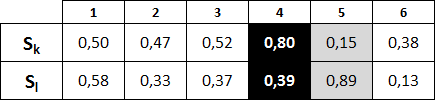
\includegraphics[width=0.70\textwidth]{figs/materiais_metodo/autovalores_com_ga/cross2004_tabelaAntes.png}
	\caption{Exemplo do \emph{crossover} de \cite{metodo2004}. Indivíduos antes da reprodução.}
	\label{fig:cross2004_tabelaAntes}
\end{figure}

O parâmetro $f$ teve seu valor determinado aleatoriamente como $f = 0,62$. Os valores de $c^{'}_{k4}$ e $c^{'}_{l4}$ ficam:

\begin{equation}\label{eq:ck4}
	\begin{array}{lccl}
		c^{'}_{kp} = & f c_{kp} & + & (1 - f) c_{lp} 						\\
		c^{'}_{k4} = & 0,62 c_{k4} & + & (1 - 0,62) c_{l4} 			\\
		c^{'}_{k4} = & 0,62 * 0,80 & + & 0,38 * 0,39 						\\		
		c^{'}_{k4} = & 0,496 & + & 0,1482	\\		
		c^{'}_{k4} = & 0,6442 &  & 
	\end{array}
\end{equation}

\begin{equation}\label{eq:cl4}
	\begin{array}{lccl}
		c^{'}_{lp} = & (1-f) c_{kp} & + & f c_{lp} 						\\
		c^{'}_{l4} = & (1-0,62) c_{k4} & + & 0,62 c_{l4} 						\\
		c^{'}_{l4} = & 0,38 * 0,80 & + & 0,62 * 0,39 						\\
		c^{'}_{l4} = & 0,304 & + & 0,2418 						\\
		c^{'}_{l4} = & 0,5458 &  & 
	\end{array}
\end{equation}

Finalmente, os valores para a posição $p = 4$ nos novos indivíduos $S^{'}_k$ e $S^{'}_l$ são

\begin{equation}\label{eq:cross2004_novo_valor_sk}
	\begin{array}{ll}
	\mbox{Novo valor na posição 4 de  } S^{'}_k & = c^{'}_{kp} c_{k,p+1} \\
								& = c^{'}_{k4} c_{k5} \\
								& = 0,6442 * 0,15	\\
								& = 0,09663	\\
								& \approx 0,1
	\end{array}
\end{equation}

\begin{equation}\label{eq:cross2004_novo_valor_sl}
	\begin{array}{ll}
	\mbox{Novo valor na posição 4 de  } S^{'}_l & = c^{'}_{lp} c_{l,p+1} \\
								& = c^{'}_{l4} c_{l5} \\
								& = 0,5458 * 0,89	\\
								& = 0,485762 \\
								& \approx  0,49
	\end{array}
\end{equation}


Na figura \ref{fig:cross2004_tabelaDepois} há os dois novos indivíduos.

\begin{figure}[htbp]
	\centering
		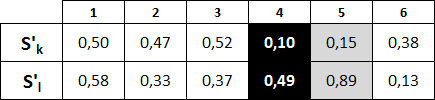
\includegraphics[width=0.70\textwidth]{figs/materiais_metodo/autovalores_com_ga/cross2004_tabelaDepois.png}
	\caption{Exemplo do \emph{crossover} de \cite{metodo2004}. Indivíduos depois da reprodução.}
	\label{fig:cross2004_tabelaDepois}
\end{figure}

%----------------------------------------------------
\subsection{\emph{Crossover} em \cite{metodo2011}}	
%----------------------------------------------------

	A representação cromossomial usada em \cite{metodo2011} é a mesma de \cite{metodo2004}, portanto, o par ($S_k$, $S_l$) é igual, assim como a probabilidade $p_c$:
	
	\begin{equation}
		\begin{array}{l}
		S_k = (c_{k1}, c_{k2}, \cdots, c_{kn})	\\
		S_l = (c_{l1}, c_{l2}, \cdots, c_{ln})	
		\end{array}
	\end{equation}
	
	Diferentemente de \cite{metodo2004}, utiliza-se o \emph{crossover} de dois pontos. Aleatoriamente escolhe-se dois inteiros, $o$ e $p$, cuja função é determinar a região do cromossomo que sofrerá miscigenação. O valor em $o$ indica o primeiro gene, e $p$ o último. Portanto, todos os genes entre os dois, incluindo eles próprios, sofrerão a ação do \emph{crossover} ($o <= c_i <= p$, $p \geq o$). Os novos indivíduos são ($S^{'}_k$, $^{'}S_l$)
	
	\begin{equation}
		\begin{array}{l}
			S^{'}_k = (c_{k1}, c_{k2}, \cdots, c^{'}_{ko}, \cdots , c^{'}_{kp}, c_{k,p+1}, \cdots, c_{kn})	\\
			S^{'}_l = (c_{l1}, c_{l2}, \cdots, c^{'}_{lo}, \cdots , c^{'}_{lp}, c_{l,p+1}, \cdots, c_{ln}).	
		\end{array}
	\end{equation}
	
	Para todos genes selecionados, a transformação ocorre da seguinte maneira ($i = o, o + 1, \cdots, p$):
	
	\begin{equation}
		\begin{array}{l}
			c^{'}_{ki} = f_c c_{ki} + (1 - f_c) c_{li}     \\
			c^{'}_{li} = (1 - f_c) c_{ki} + f_c c_{li}
		\end{array}
	\end{equation}
	onde $f_c$ é dado por
	
	\begin{equation}
		f_c = 0,75 + 0,25r,
	\end{equation}
	sendo $r$ um número aleatório ($0 \leq r \leq 1$). Assim como o parâmetro $f$ de \cite{metodo2004}, $f_c$ faz o papel da mistura que cria nova informação.
	
	\textbf{Exemplo}.
	
	
	Usei os mesmos indivíduos da figura \ref{fig:cross2004_tabelaAntes}. Os parâmetros $o$ e $p$ foram escolhidos no intervalo [1,6] e têm valores $o = 2$ e $p = 4$. Portanto, no \emph{string} $S_k$ os elementos que sofrerão alteração são $c_{k2} = 0,47$, $c_{k3} = 0,52$ e $c_{k4} = 0,80$. Eles se misturarão com os elementos $c_{l2} = 0,33$, $c_{l3} = 0,37$ e $c_{l4} = 0,39$ de $S_l$. Aleatoriamente obtive $r = 0,2$, que leva a $f_c = 0,80$.
	
	\begin{figure}[htbp]
	\centering
		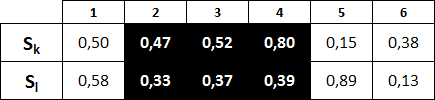
\includegraphics[width=0.70\textwidth]{figs/materiais_metodo/autovalores_com_ga/cross2011_tabelaAntes.png}
	\caption{Exemplo do \emph{crossover} de \cite{metodo2011}. Indivíduos antes da reprodução.}
	\label{fig:cross2011_tabelaAntes}
\end{figure}
	
	Os elementos $c^{'}_{ki}$ são:
	
	\begin{equation}
		\begin{array}{llcl}
			c^{'}_{k2}	& = f_c c_{k2} 		& + & (1- f_c) c_{l2} \\
									& = 0,80 * 0,47		& + &	(1 - 0,80) * 0,33 \\
									& = 0,376					& + & 0,2 * 0,33	\\
									& = 0,376					& + & 0,066	\\
									& = 0,442 \\
									& \approx 0,44
		\end{array}
	\end{equation}
	
	
	\begin{equation}
		\begin{array}{llcl}
			c^{'}_{k3}	& = f_c c_{k3} 		& + & (1- f_c) c_{l3} \\
									& = 0,80 * 0,52		& + &	(1 - 0,80) * 0,37 \\
									& = 0,416					& + & 0,2 * 0,37	\\
									& = 0,416					& + & 0,074	\\
									& = 0,49
		\end{array}
	\end{equation}
	
	
	\begin{equation}
		\begin{array}{llcl}
			c^{'}_{k4}	& = f_c c_{k4} 		& + & (1- f_c) c_{l4} \\
									& = 0,80 * 0,80		& + &	(1 - 0,80) * 0,39 \\
									& = 0,64					& + & 0,2 * 0,39	\\
									& = 0,64					& + & 0,078	\\
									& = 0,718 \\
									& \approx 0,72
		\end{array}
	\end{equation}
	
	
	Os elementos $c^{'}_{li}$ são:
	
	\begin{equation}
		\begin{array}{llcl}
			c^{'}_{l2}	& = (1 - f_c) c_{k2} 		& + & f_c c_{l2} \\
									& = (1 - 0,80) * 0,47		& + &	0,80 * 0,33 \\
									& = 0,2 * 0,47					& + & 0,264	\\
									& = 0,094					& + & 0,264	\\
									& = 0,358 \\
									& \approx 0,36
		\end{array}
	\end{equation}
	
	\begin{equation}
		\begin{array}{llcl}
			c^{'}_{l3}	& = (1 - f_c) c_{k3} 		& + & f_c c_{l3} \\
									& = (1 - 0,80) * 0,52		& + &	0,80 * 0,37 \\
									& = 0,2 * 0,52					& + & 0,296	\\
									& = 0,104								& + & 0,296	\\
									& = 0,40									
		\end{array}
	\end{equation}
	
	
	\begin{equation}
		\begin{array}{llcl}
			c^{'}_{l4}	& = (1 - f_c) c_{k4} 		& + & f_c c_{l4} \\
									& = (1 - 0,80) * 0,80		& + &	0,80 * 0,39 \\
									& = 0,2 * 0,80					& + & 0,312	\\
									& = 0,16								& + & 0,312	\\
									& = 0,472 \\
									& \approx 0,47
		\end{array}
	\end{equation}
	
	Os novos indivíduos estão na figura \ref{fig:cross2011_tabelaDepois}.
		
	\begin{figure}[htbp]
	\centering
		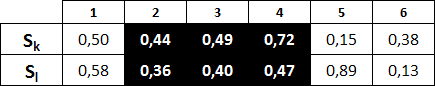
\includegraphics[width=0.70\textwidth]{figs/materiais_metodo/autovalores_com_ga/cross2011_tabelaDepois.png}
	\caption{Exemplo do \emph{crossover} de \cite{metodo2011}. Indivíduos depois da reprodução.}
	\label{fig:cross2011_tabelaDepois}
\end{figure}
	
	
%----------------------------------------------------
\subsection{\emph{Crossover} utilizado}
\label{sec:crossover_utilizado}
%----------------------------------------------------

	A quantidade de nova informação não é escalável com o tamanho do cromossomo no \emph{crossover} de \cite{metodo2004}. Ele altera apenas uma posição (locus) de cada indivíduo, independentemente do tamanho do cromossomo. Por exemplo, se a ordem do Hamiltoniano for $n = 100$, o \emph{string} terá 100 elementos, mas apenas um sofrerá alteração. O mesmo aconteceria para $n = 1.000$, 10.000 e assim por diante.
	
	Ainda sobre o artigo de 2004, é impossível haver troca de informação na última posição. O parâmetro $p$, obtido aleatoriamente, dá a posição na qual ocorrerá o \emph{crossover}. Porém, parte do cálculo envolve os elementos $c_{k,p+1}$ e $c_{l,p+1}$. Note o índice $p+1$. Como a posição máxima é $n$, o maior índice possível para estes elementos é $p + 1 = n$, impondo o limite $p \leq n - 1$. Nos exemplos apresentados, $n = 6$, $p \leq 5$ e, portanto, a posição $6$ nunca será escolhida.
	
	Isso pode dificultar a busca. Suponha que uma solução precise do valor 23 no último coeficiente do cromossomo ($c_n = 0,23$). Se nenhum indivíduo da população inicial já tiver nascido com ele, esse valor nunca aparecerá por meio do \emph{crossover}. Resta como esperança a Mutação, porém, por definição, ela tem baixa probabilidade \cite{Linden2008}. Também não há garantia de que, após muitas gerações com sucessivas operações de \emph{crossover}, mutação e seleção, haverá um indivíduo na população que, além de ter 0,23 na última posição, possua os outros $(n-1)$ primeiros elementos necessários.
		
		O \emph{crossover} de \cite{metodo2004} é um caso especial do \emph{crossover} de \cite{metodo2011}. O operador de reprodução de \cite{metodo2011} é o clássico \emph{crossover} de dois pontos \cite{Linden2008}. Nele, $p \geq o$, e, se $o = p$, há mistura em apenas uma posição do \emph{string}, exatamente o que acontece em \cite{metodo2004}. Como $1 \leq o \leq n$ e $1 \leq p \leq n$, o último gene também está sujeito à operação, e o problema citado no parágrafo anterior não existe.
		
	Pelo que expus acima, escolhi utilizar o \emph{crossover} de \cite{metodo2011}, mas com uma pequena modificação. No cálculo dos novos coeficientes $c^{'}_{i}$, em vez do parâmetro $f_c$, usei o $f$ conforme definido em \cite{metodo2004}. O $f$ pode variar entre $0$ e $1$, enquanto o $f_c$, além de necessitar do parâmetro adicional $r$, é limitado apenas entre $0,75$ e $1$. Assim, acredito que $f$ seja mais abrangente como parâmetro de mistura e criação de nova informação.
	
	\textbf{\emph{Crossover} utilizado}
	
	A seguir apresento sinteticamente a estrutura do \emph{crossover} utilizado. Um par de indivíduos $(S_k, S_l)$
	
	\begin{equation}
		\begin{array}{l}
			S_k = (c_{k1}, c_{k2}, \cdots, c_{kn})	\\
			S_l = (c_{l1}, c_{l2}, \cdots, c_{ln})	
		\end{array}
	\end{equation}
	é obtido aleatoriamente da população. Com probabilidade $p_c$, a operação de \emph{crossover} acontece. Dois pontos de corte $o$ e $p$ são obtidos, também aleatoriamente, gerando os novos \emph{strings} $S^{'}_k$ e $S^{'}_l$ na forma
		
	\begin{equation}
		\begin{array}{l}
			S^{'}_k = (c_{k1}, c_{k2}, \cdots, c^{'}_{ko}, \cdots , c^{'}_{kp}, c_{k,p+1}, \cdots, c_{kn})	\\
			S^{'}_l = (c_{l1}, c_{l2}, \cdots, c^{'}_{lo}, \cdots , c^{'}_{lp}, c_{l,p+1}, \cdots, c_{ln}),
		\end{array}
	\end{equation}
	onde
	
	\begin{equation}\label{eq:recombinacao}
		\begin{array}{l}
			c^{'}_{ki} = f c_{ki} + (1 - f) c_{li}     \\
			c^{'}_{li} = (1 - f) c_{ki} + f c_{li}
		\end{array}
	\end{equation}
	e
	
	\begin{equation}
	0 \leq f \leq 1 \mbox{       (obtido aleatoriamente)}
	\end{equation}

%-------------------------------------------------------
\section{Mutação}
%-------------------------------------------------------

	O operador Mutação é semelhante nos dois artigos. Todos os cromossomos estão sujeitos à mutação. Se um indivíduo $k$ sofre mutação no gene $q$, o antigo valor $c^{'}_{kq}$ é alterado para $c^{''}_{kq}$ com a seguinte equação:

		\begin{equation}\label{eq:mutacao}
			c^{''}_{kq} = c^{'}_{kq} + (-1)^{L} r \Delta,
		\end{equation}
		onde $L$ é um número inteiro, $r$ um número aleatório ($0 \leq r \leq 1$) e $\Delta$ é a intensidade da mutação.
		
		
	Não ficou claro para mim qual a relação entre a probabilidade $p_m$ e como será a mutação no artigo \cite{metodo2004}. Os autores dizem que todos os \emph{indivíduos} estão sujeitos ao operador, mas não citam quais \emph{genes} podem sofrer mutação. Essa informação está explícita em \cite{metodo2011}, que permite mutação, caso aconteça, em apenas um gene de cada indivíduo. Ou seja, se houver mutação logo no primeiro gene de um cromossomo, o algoritmo parte para o próximo indivíduo.
	
	Assumi que no artigo \cite{metodo2004} os autores utilizaram o operador clássico. Conforme a literatura \cite{Mitchell98, Linden2008} o operador clássico de mutação age com probabilidade $p_m$ em cada gene, de maneira individual e independente. Ou seja, se um gene $c_{k,j}$ sofreu ou não mutação, essa informação não é utilizada para avaliar a ocorrência de mutação no próximo gene $c_{k,j+1}$. Portanto, a probabilidade de cada \emph{gene} sofrer mutação é $p_m$, mas a probabilidade $P_m$ de um \emph{indivíduo} sofrer mutação é, na verdade, $P_m = n*p_m$. Quanto maior o $n$, mais provável ocorrer a mutação, o que me parece razoável. Mutação é causada principalmente por erros de cópia do DNA. Quanto maior a fita, mais chance de acontecer erro.

	Há diferença na intensidade da mutação $\Delta$. No trabalho de 2004 ela é pequena ($10^{-2}-10^{-3}$) e mantida constante. Já no segundo artigo ela é proporcional ao melhor \emph{fitness} $f_t$ da geração atual $t$, e dada pela equação \ref{eq:Delta2011}. Como o \emph{fitness} começa pequeno e termina próximo de 1, $\Delta \rightarrow 0$ à medida que $f \rightarrow 1$.

\begin{equation}\label{eq:Delta2011}
	\Delta^{(t)}_m =  1 - f_t.
\end{equation}	

	Não fiquei confortável com a definição da equação \ref{eq:Delta2011}, por isso usei a intensidade $\Delta$ constante de \cite{metodo2004}. No início de um GA a criação de variabilidade genética é dominada pelo \emph{crossover}. No final, como os indivíduos são parecidos, fica a cargo da mutação fazer isso. A intensidade da mutação deve ser pequena e, se não for constante, é desejável que cresça com o tempo, justamente porque o papel da mutação passa a ser dominante na variabilidade comparado com o \emph{crossover} \cite{Linden2008}. Os autores de \cite{metodo2011} fazem o inverso. Como dito anteriormente, $\Delta$ diminui com o tempo, mas eles não justificam porque optaram por esse comportamento.
	
	Com relação à probabilidade de mutação, optei novamente a favor de \cite{metodo2004}. Ambos os trabalhos utilizam valor constante de $p_m$. Entretanto, em \cite{metodo2011} $p_m$ é inversamente proporcional ao tamanho do cromossomo $n$ (equação \ref{eq:probM2011}). Na prática, quanto maior a ordem $n$ do Hamiltoniano, menor a probabilidade de mutação, e no artigo não há justificativa para essa escolha. Fiquei com a probabilidade constante, discutida em livros tradicionais de GA \cite{Mitchell98, Linden2008}.

	\begin{equation}\label{eq:probM2011}
		p_m = 4.0/n
	\end{equation}


	\textbf{Mutação utilizada.}
	
	Abaixo resumo a estrutura da Mutação implementada na dissertação.
	
	
	\begin{itemize}
		\item \textbf{Probabilidade de mutação $p_m$}
			\begin{itemize}
				\item Constante.
				\item Um dos parâmetros do algoritmo.
				\item Pode ter qualquer valor $0 \leq p_m \leq 1$.
			\end{itemize}
		\item \textbf{Equação da mutação}.
			\begin{itemize}
				\item No indivíduo $S$, transforma o valor $c^{'}_{kq}$ do gene $q$ no novo valor $c^{''}_{kq}$.
				\item Equação: $c^{''}_{kq} = c^{'}_{kq} + (-1)^{L} r \Delta$
				\item Parâmetro $L$: inteiro aleatório.
				\item Parâmetro $r$: aleatório ($0 \leq r \leq 1$).
				\item Intensidade de mutação $\Delta$: Constante. Valores pequenos ($10^{-3}-10^{-2}$).
			\end{itemize}
	\end{itemize}
	

%-------------------------------------------------------
\section{Fluxograma do algoritmo implementado}
%-------------------------------------------------------

	O algoritmo genético seguiu a estrutura de um GA básico \cite{Mitchell98, Linden2008}. Após gerar a população inicial, Avaliação, Seleção, \emph{Crossover} e Mutação são executados nessa sequência até que uma condição de parada seja atingida.
	
	Na figura \ref{fig:fluxo} está o fluxograma. Ele não é um diagrama completo do \emph{software} desenvolvido, mas é útil para ter a visão geral do algoritmo.

\begin{figure}[htbp]
	\centering
		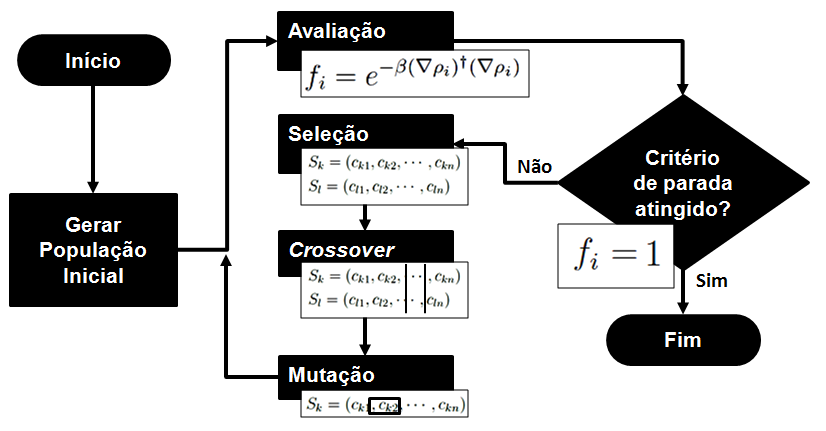
\includegraphics[width=0.90\textwidth]{figs/materiais_metodo/autovalores_com_ga/fluxo.png}
	\caption{Fluxo algoritmo genético}
	\label{fig:fluxo}
\end{figure}
\chapter{Metodologia\label{cap:metodologia}}
	
	A metodologia foi baseada em estudo aprofundado de Algoritmos Genéticos e no desenvolvimento de um \emph{software} confiável para execução do modelo. Ambos são apresentados
nas seções seguintes.

%========================================================
\section{Algoritmos Genéticos}\label{seq:medologia_ga}
%========================================================
	
	Iniciei os estudos em Algoritmos Genéticos pelos livros \cite{Mitchell98} e \cite{Linden2008} e, antes de partir para o trabalho da dissertação em si, trabalhei com três problemas completamente distintos.
	
	O primeiro foi o ONEMAX \cite{onemaxNaGPU}, desenvolvido ``do zero'', em Linguagem C. Considerado o \emph{hello world} do GA, tem representação cromossomial binária, o \emph{fitness} é a soma dos \emph{bits} de cada indivíduo e o objetivo é obter um indivíduo com o maior número de '1' possível. Com ele pude estudar os parâmetros de um GA simples, como número de indivíduos e a probabilidade de \emph{crossover}, e verificar a influência de cada um na qualidade da solução, convergência, desempenho, evolução do \emph{fitness} etc. Uma versão paralelizada em CUDA foi apresentada em evento de computação de alto desempenho \cite{ERAD12} e encontra-se no apêndice \ref{apdx:oneMaxNaGPU}.
	
	\begin{figure}[htbp]
		\centering
			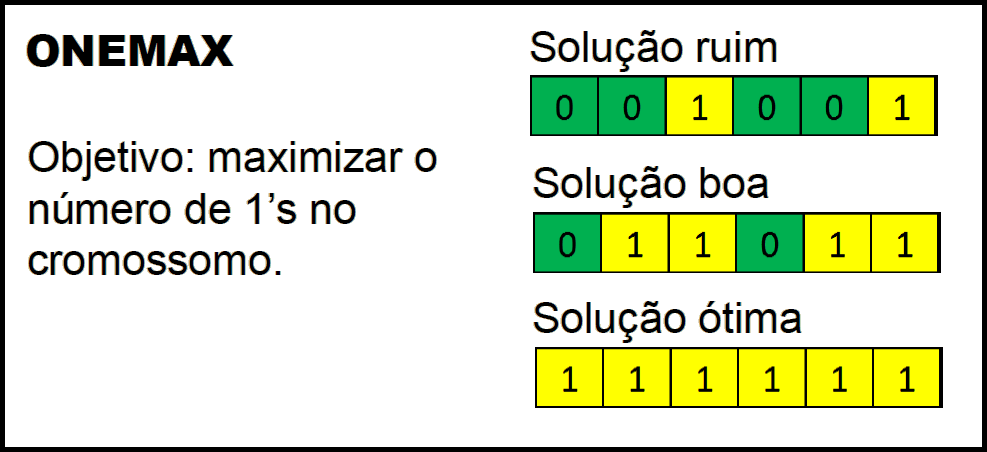
\includegraphics[width=0.60\textwidth]{figs/resultados/onemax/onemax_objetivo.png}
		\caption{ONEMAX: representação cromossomial, \emph{fitness} e objetivo.}
		\label{fig:onemax_objetivo_metodologia}
	\end{figure}
	
	Tendo a estrutura básica do ONEMAX, o próximo passo foi tentar fazer um modelo. Abordei o Problema das Oito Rainhas, que consiste em posicionar oito rainhas em um tabuleiro de xadrez de modo que não se ataquem. Sem nenhuma referência externa, propus um modelo de GA que conseguiu chegar em algumas soluções \cite{qualificacao_adriano}. Uma delas está na figura \ref{fig:OitoRainhasSolucao}.
	
	\begin{figure}[htbp]
		\centering
			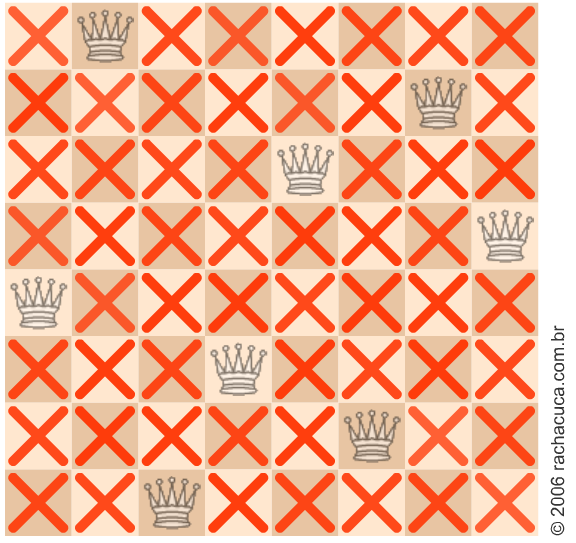
\includegraphics[width=0.30\textwidth]{figs/materiais_metodo/ga/OitoRainhasSolucao.png}
		\caption{Uma solução para o Problema das 8 Rainhas.}
		\label{fig:OitoRainhasSolucao}
	\end{figure}
	
	Tratando o tabuleiro de xadrez como um plano cartesiano, a representação cromossomial era um \emph{string} com os oito pares de coordenadas $(x,y)$. Cada coordenada gerava uma matriz característica de 0's e 1's que, quando somadas, resultava em uma matriz com a informação da quantidade $c$ de ataques que cada rainha sofreu. O objetivo, portanto, era encontrar um indivíduo que levasse a $c = 0$. A função de avaliação foi definida como $f = 1/(1 + c)$.
	
	Criar um modelo para o Oito Rainhas foi importante para o entendimento do elo entre um GA e o problema a ser resolvido. Essa ligação encontra-se na representação cromossomial e na função de avaliação. Defini ambas de maneira adequada, mas a representação cromossomial apresentou um problema: nada impede de haver pontos $(x,y)$ repetidos no cromossomo. Em outras palavras, ela permite que duas rainhas sejam colocadas na mesma posição do tabulareiro, o que é proibido no xadrez. 
	
	Por fim, utilizei GA na criação de um robô, chamado \emph{Genético}, para ser testado contra os campeões do torneio de Robocode da Faculdade de Tecnologia da Unicamp\footnote{\texttt{http://torneiorobocode.orgfree.com/torneio-ft.php}}. Robocode é um jogo\footnote{\texttt{http://robocode.sourceforge.net/}}, cujo objetivo é programar um tanque de guerra robô para competir contra outros robôs em uma arena de batalha. Ele começou como um projeto pessoal no ano 2000 e depois foi incorporado pela IBM\footnote{\texttt{http://robocode.sourceforge.net/docs/ReadMe.html}}. Atualmente é um projeto de código aberto.
	
	\begin{figure}[htbp]
		\centering
			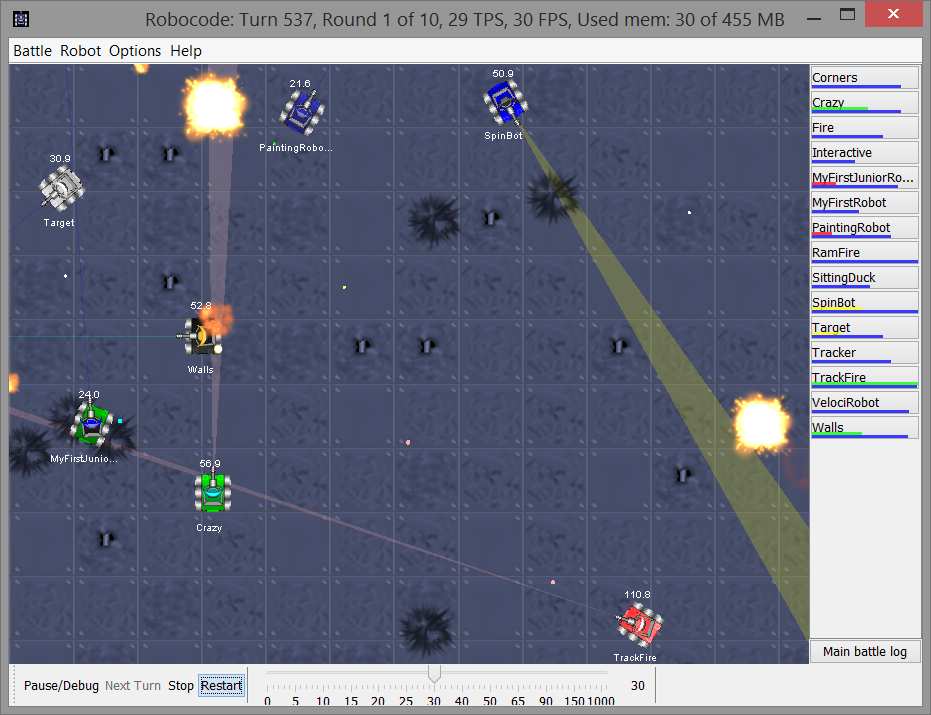
\includegraphics[width=0.50\textwidth]{figs/materiais_metodo/ga/Robocode_Battle_Field.PNG}
		\caption{Arena de batalha do Robocode.}
		\label{fig:Robocode}
	\end{figure}
	
	Baseei-me no artigo \cite{robocodeGA}, publicado em um congresso de computação evolutiva da IEEE. As primeiras versões do \emph{Genético} não travaram boas batalhas. Alterei o \emph{fitness} e o processo de treinamento. Na versão final ele foi capaz de vencer os robôs que ficaram em primeiro e terceiro lugares no torneio daquele ano (o segundo lugar não estava disponível para \emph{download}). O \emph{Genético} vencia, inclusive, contra os dois simultaneamente \cite{robocodeGA_adriano}.
	

%========================================================
\section{\emph{Software}}
%========================================================

	O \emph{software} utilizado foi totalmente desenvolvido por mim, e há razões metodológicas que justificam essa escolha. Obtive bons resultados criando os próprios programas nos estudos iniciais de GA. Eles foram fundamentais para que eu soubesse exatamente o que estava acontecendo durante a execução. Quis ter esse controle total também sobre o programa que executaria o GA proposto para esta dissertação. Ele foi escrito em Linguagem C, utilizando apenas quatro bibliotecas padrão: \texttt{stdio.h}, \texttt{stdlib.h}, \texttt{time.h} e \texttt{math.h}. Portanto, é totalmente portável para os sistemas operacionais que possuem um compilador C$++$. Além disso, C é a linguagem nativa da arquitetura CUDA, o que facilitará sua paralelização. O código está disponível na internet para qualquer um utilizar, testar e, inclusive, melhorar\footnote{\texttt{https://github.com/prietoab/msc\_code}}. Caso isso aconteça, peço apenas que cite esta dissertação.
	
	Tive muito cuidado com a confiabilidade dos resultados. Quando opta-se por não gerá-la automaticamente, a \emph{semente} dos números pseudo-aleatórios é um dos parâmetros de entrada. Duas execuções com os mesmos parâmetros, incluindo a semente, levam a exatamente os mesmos resultados. Por isso nas tabelas e gráficos deixei explícito seu valor. Os gráficos encontrados em \cite{metodo2004} e \cite{metodo2011} referem-se ao maior \emph{fitness} (e $\rho$ associado) de cada geração. O programa gera essa informação, mas também exibe as médias dessas variáveis. De acordo com \cite{Mitchell98}, uma teoria geral para entender e prever o comportamento dos GAs seria análoga à Mecânica Estatística na Física. Ao contrário de lidar com grande número de componentes do sistema, como a composição genética exata de cada população, tal abordagem trabalha com uma estatística mais ``macroscópica'', como o \emph{fitness} médio da população. Portanto, tanto os critérios de parada do programa quanto a minha análise foram baseadas em médias.
	
%---------------------------------------------------
\subsection{Como utilizar o programa}
%---------------------------------------------------	
	
	Para utilizar o \emph{software} basta compilar o arquivo \texttt{Serial\_novo.c} (será necessário alterar o diretório no \emph{include} das bibliotecas que desenvolvi).
	
		A execução dá-se via linha de comando passando os parâmetros necessários. Porém, como são muitos parâmetros, é aconselhável a utilização de um arquivo de \emph{script}. Assim é possível criar processos de varredura para variar os parâmetros desejados ou repetir várias execuções. Fiz isso para automatizar o estudo e ter dados suficientes para análise. Na figura \ref{fig:script_windows} há um exemplo de \emph{script} Windows para fazer execuções variando o número de genes.
			
		\begin{figure}[htbp]
			\centering
				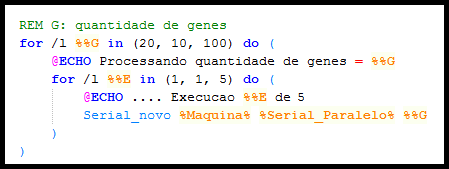
\includegraphics{figs/materiais_metodo/software/script_windows.png}
			\caption{Exemplo de \emph{script} Windows para fazer execuções variando o número de genes.}
			\label{fig:script_windows}
		\end{figure}

	Não é necessário ter uma matriz para execução. Por meio do parâmetro \emph{Tamanho do cromossomo} (seção \ref{sec:listaParametros}) o programa gera automaticamente uma matriz de Coope \cite{Coope1977}, definida na equação \ref{eq:MatrizCoope}. Essa matriz, que não possui significado físico, foi escolhida pois também é utilizada nos testes de \cite{metodo2011}.
	
	\begin{equation}\label{eq:MatrizCoope}
		\begin{array}{ccl}
			H(i,i) = 2i - 1 			& , & i = 1, 2, ..., n. \\
														&		&		\\
			H(i,j) = H(j,i) = 1		& , & i \neq j; \\
														&		& i = 1, 2, ..., n; \\
														&		& j = 1, 2, ..., n.
		\end{array}
	\end{equation}
	
%---------------------------------------------------
\subsection{Informações de saída}
%---------------------------------------------------	
		
Há cinco grupos de informações na saída do programa. Usados em conjunto dão um panorama do algoritmo genético. Para apenas um deles (Estatística) um arquivo texto é gerado automaticamente. Os outros são exibidos na tela. Para alterar a saída padrão para um arquivo texto, é necessário utilizar o caractere de redirecionamento da saída padrão\footnote{No Windows, Linux e Unix esse caractere é o ``>''. No Linux, por exemplo, o comando ``\texttt{ls > dirs.txt}'' lista o conteúdo do diretório atual e armazena no arquivo \texttt{dirs.txt}.}.

\begin{enumerate}

	\item \textbf{Cabeçalho}
	
		Contém todos os parâmetros de execução recebidos na linha de comando. Impresso na tela.
	
	\item \textbf{Comportamento do \emph{fitness}}
	
		Imprime na tela, para cada geração, além de alguns parâmetros de execução, as seguintes informações: 
		
		\begin{itemize}
			\item $\rho$ mínimo
			\item $\rho$ médio (<$\rho$>)
			\item \emph{fitness} médio (<\emph{fitness}>)
			\item Maior \emph{fitness}
			\item $\rho$ associado ao maior \emph{fitness}
			\item <$|\nabla \rho|^2$>
			\item Posição do melhor indivíduo
		\end{itemize}

	\item \textbf{Tempos de processamento}
	
		Imprime na tela uma estimativa para o tempo de processamento (em \emph{clocks}) para cada operador. Se o programa foi executado por 200 gerações, haverá 200 tempos de processamento para o \emph{fitness}, seleção, \emph{crossover} e mutação.
		
	\item \textbf{Geração final}
	
				Impressão de todos os indivíduos da última geração. 
	
	\item \textbf{Estatística}
	
				A cada execução é criado (ou atualizado caso já exista) um arquivo chamado \texttt{estatistica.txt}. Nele, além de todos os parâmetros, há informações relacionadas à geração que atingiu algum critério de parada. Por exemplo, além do próprio número da última geração, há o \emph{fitness} médio, o maior \emph{fitness}, o $\rho$ associado ao maior \emph{fitness}, o $\rho$ médio e o tempo total de processamento do programa.
	
\end{enumerate}
	
%---------------------------------------------------
\subsection{Lista dos arquivos fonte}
%---------------------------------------------------
	
	O programa é pequeno ($\approx$ 2500 linhas), e está distribuído em seis arquivos, um principal e cinco bibliotecas:
	
	\begin{itemize}
		\item \textbf{Serial\_novo.c}
		
		Arquivo principal. Contém o fluxo do GA (figura \ref{fig:fluxo}).
		
		\item \textbf{Estruturas.h}
		
		Contém as estruturas de dados e uma função que retorna automaticamente o parâmetro $\beta$ do \emph{fitness} (seção \ref{sec:eq_lambda}).
		
		\item \textbf{Algebra\_Linear\_serial.h}
		
		Mutiplicação e subtração de matrizes.
		
		\item \textbf{Estatistica.h}
		
		Média, variância e desvios do Quociente de Rayleigh.
		
		\item \textbf{Auxiliares\_serial.h}
		
		Números pseudo-aleatórios, alocação de memória para indivíduos na população.
		
		\item \textbf{GA\_Serial.h}
		
		Contém as funções do Algoritmo Genético. A maioria do código está nessa biblioteca.	
		
	\end{itemize}
					
%---------------------------------------------------
\subsection{Lista dos parâmetros de execução}
\label{sec:listaParametros}
%---------------------------------------------------
	\begin{enumerate}
		\item \textbf{Código da máquina}.
		
				Número inteiro, utilizado para identificar o computador que o programa foi executado. Útil para comparar as execuções em computadores diferentes. Por exemplo, se há quatro computadores A, B, C e D, é possível classificá-los como A = 0, B = 1, C = 2, D = 3.
				
		\item \textbf{Serial ou Paralelo}?
		
				Número inteiro. Determina se a execução será serial (= 0) ou paralela (= 1). A atual versão permite apenas execução serial. Portanto, esse parâmetro pode ser fixado em zero.
				
		\item \textbf{Tamanho do cromossomo (ordem da matriz de Coope)}.
		
				Número inteiro. Determina a ordem da matriz de Coope. Inserir 200 nesse parâmetro gera uma matriz de Coope de tamanho 200 x 200.
			
		\item \textbf{Quantidade máxima de gerações}.
		
				Número inteiro. Um dos critérios de parada. Para evitar que o programa entre em um \emph{loop} infinito caso não haja convergência para uma solução. Se definida como 100, o programa executará, no máximo, 100 iterações de Avaliação, Seleção, \emph{Crossover} e Mutação.
		
		\item \textbf{Quantidade de indivíduos na população}.
		
		Número inteiro. Determina a quantidade de indivíduos em cada população.
		
		\item \textbf{Tipo do Fitness}.
		
		Número inteiro. O programa pode trabalhar com cinco tipos de \emph{fitness}. Dois deles são os apresentados na seção \ref{sec:fitness_metodo}. Qualquer código diferente dos apresentados abaixo faz com que o \emph{fitness} seja definido como $f = -1$.
		
			\begin{itemize}
				\item Tipo 0 \cite{metodo2011}:
				
					\begin{equation}
					f = e^{-\beta(\rho - E_L)^2}
					\end{equation}
				
				\item Tipo 1 \cite{metodo2004}:
				
					\begin{equation}
					f = e^{-\beta |\nabla \rho|^2}
					\end{equation}
					
				\item Tipo 2:
				
					\begin{equation}
					f = e^{-\beta [(\rho - E_L)^2 + |\nabla \rho|^2]}
					\end{equation}
					
				\item Tipo 3:
				
					\begin{equation}
					f = e^{-\beta |\nabla \rho|}
					\end{equation}
		
			\item Tipo 4:
				
					\begin{equation}
					f = e^{-\beta [(\rho - E_L)^2 + |\nabla \rho|]}
					\end{equation}
			\end{itemize}
			
		\item \textbf{Tipo do Fitness Paralelo}.
		
				Número inteiro. A atual versão permite apenas execução serial. Portanto, esse parâmetro pode ser fixado em zero.
		
		\item \textbf{Tamanho do Torneio}
		
			Número inteiro. Define a quantidade de indivíduos selecionados para o torneio na Seleção.
		
		\item \textbf{Probabilidade do \emph{Crossover}}.
		
			Número real. Define, em porcentagem, a probabilidade de \emph{Crossover}. Exemplo: 80.5 = 80,5\%.
		
		\item \textbf{Quantidade de Pontos de Corte}.
		
			Número inteiro. Na versão atual a quantidade de pontos de corte foi fixada em dois conforme o operador de \emph{crossover} definido na seção \ref{sec:crossover_utilizado}. Pode ser mantido como zero.
		
		\item \textbf{Probabilidade de Mutação}.
		
		Número real. Define, em porcentagem, a probabilidade de mutação. Exemplo: 12.7 = 12,7\%.
		
		\item \textbf{Intensidade da Mutação - $\Delta$}.
		
			Número real. Define o parâmetro $\Delta$ utilizado no \emph{crossover}. É dividido por dez. Exemplo: $1.2$ no parâmetro $\rightarrow 0,12$ no $\Delta$.
		
		\item \textbf{Valor para $\beta$}.
		
		Número real. Define o valor do parâmetro $\beta$ do \emph{fitness}. Se for configurado como $-1$, um valor adequado para $\beta$ é gerado automaticamente.
		
		\item \textbf{Valor para $E_L$}.
		
		Número real. Define um limite inferior para o autovalor mínimo ($E_0$) nos \emph{fitness} de tipo 0, 2 e 4. 
		
		\item \textbf{Precisão - $\xi$}.
		
		Número real. Define a precisão dos critérios de parada. O programa termina se a variável alvo é menor ou igual a $\xi$. Depende do tipo de \emph{fitness}.
		
		Condições de parada em função do \emph{fitness} ($<x>$ significa valor médio de $x$):
				
		\begin{itemize}
			\item Fitness tipos 0, 2 e 4:
						
			\begin{equation}\label{eq:criterioParada024}
				\begin{array}{ccll}
				<|\nabla \rho|> & \leq & \xi & \mbox{  ou} \\
				| <\rho> - E_L | & \leq & \xi &
				\end{array}
			\end{equation}
			
			
			\item Fitness tipos 1 e 3:
			
			\begin{equation}\label{eq:criterioParada13}
				\begin{array}{ccll}
					<|\nabla \rho|> & \leq & \xi &
				\end{array}
			\end{equation}
			
		\end{itemize}
		
		\item \textbf{Imprime comportamento do \emph{Fitness}}?
		
		Se configurado como Verdadeiro (1), imprime na saída padrão as variáveis de interesse para estudar o comportamento do \emph{fitness}. 
		
			0: \emph{Falso}. Não imprime.
			
			1: \emph{Verdadeiro}. Imprime.
		
		\item \textbf{Imprime tempos de execução}?
		
			Número inteiro. Se configurado como Verdadeiro (1), imprime na saída padrão os tempos estimados de execução (em \emph{clocks} do processador) das funções e operadores.
			
			
			0: \emph{Falso}. Não imprime.
			
			1: \emph{Verdadeiro}. Imprime.
			
		
		\item \textbf{Gera nova semente para números pseudo-aleatrórios}?
		
		Número inteiro. Se configurado como Verdadeiro (1), o programa cria uma nova semente para os números pseudo-aleatórios. Caso contrário, a semente definida no próximo parâmetro é utilizada.
		
		0: \emph{Falso}. Utiliza semente definida no parâmetro \emph{Semente}.
		
		1: \emph{Verdadeiro}. Cria uma nova semente. O parâmetro \emph{Semente} é ignorado.
		
		\item \textbf{Semente dos números pseudo-aleatrórios}.
		
		Número inteiro. Define a semente dos números pseudo-aleatórios. Depende do parâmetro anterior.
		
		\item \textbf{Tipo do cálculo de $\nabla \rho$}.
		
		Deve ser configurado como 1.
		
		Nas versões iniciais $\nabla \rho$ era calculado literalmente como na equação \ref{eq:grad_rho_metodo}, exigindo o uso de uma matriz identidade ($I$) da ordem do Hamiltoniano. A equação foi reescrita internamente de modo que $I$ não fosse necessária, liberando memória e fazendo menos operações. Usar ou não $I$ leva aos mesmos resultados.
		
		0: Utiliza matriz identidade.
		
		1: Não utiliza matriz identidade (libera memória e faz menos operações).
		
	\end{enumerate}
	
%---------------------------------------------------
\subsection{Estruturas de Dados}
%---------------------------------------------------	

	Cinco estruturas de dados formam a base do programa. Elas estão definidas no arquivo Estruturas.h.
	
%----
\subsubsection{parametrosPrograma}
%----

	Responsável por armazenar os parâmetros de execução, descritos na seção \ref{sec:listaParametros}.
	

\vspace{1 cm}	
\begin{lstlisting}
struct parametrosPrograma {
  unsigned short int parmMaquina;
  unsigned short int parmSerial_ou_Paralelo;
  unsigned short int parmQtdeGenes;
  unsigned long int parmQtdeMaxGeracoes;
  unsigned short int parmQtdeIndividuos;
  char parmTipoFitnessEquacao;
  char parmTipoFitnessParalelo;
  char parmTipoCalculoGradRho;
  char parmTamanhoTorneio;
  double parmProbCrossOver;
  unsigned short int parmQtdePontosCorte;
  double parmProbMutacao;
  double parmIntensidadeMutacao;
  double parmLambda;
  double parmRhoMinimo;
  double parmTolerancia;
  unsigned short int parmFlagImprimeComportamentoFitness;
  unsigned short int parmFlagImprimeTempo;
  unsigned short int parmFlagNovaSemente;
  unsigned long int parmSemente;
};
\end{lstlisting}
\vspace{1 cm}

%----
\subsubsection{parametros\_Metodo}
%----

	Armazena os parâmetros do \emph{fitness}, $\beta$ e $E_0$.


\vspace{1 cm}	
\begin{lstlisting}
struct parametros_Metodo {
  double lambda;
  double rho_minimo;
};
\end{lstlisting}
\vspace{1 cm}

%----
\subsubsection{parametros}
%----
	
	Parâmetros do algoritmo genético.
	

\vspace{1 cm}	
\begin{lstlisting}
struct parametros {
  unsigned short int numGenes;
  unsigned short int numIndividuos;
  double probCrossOver;
  double probMutacao;
  double intensidadeMutacao;
  char tamanho_torneio;
  unsigned short int qtde_Pontos_de_Corte;
};
\end{lstlisting}
\vspace{1 cm}

%----
\subsubsection{individual}
%----

	Essa estrutura representa o cromossomo, o indivíduo, do algoritmo genético.
	
	\textbf{\texttt{cociente\_Rayleigh}}: $\rho_i$.
	
  \textbf{\texttt{grad\_elevado\_ao\_quadrado}}: $|\nabla \rho_i|^2$.
	
  \textbf{\texttt{rho\_menos\_rho0\_ao\_quadrado}}: $(\rho_i - E_0)^2$.
	
  \textbf{\texttt{Numerador}}: Recebe o retorno do cálculo $C_i^\dagger H C_i$, utilizado na equação \ref{eq:rho-GA}, seção \ref{sec:fitness_metodo}.
  
	\textbf{\texttt{CtC}}: Recebe o produto escalar de $C{_i}^{\dag}C_i$, utilizado no cálculo da equação \ref{eq:rho-GA}, seção \ref{sec:fitness_metodo}.
  
	\textbf{\texttt{inverso\_de\_CtC}}: $(C_i^{\dag}C_i)^{-1}$.
  
	\textbf{\texttt{fitness}}: recebe o valor do \emph{fitness} do indivíduo, independente do tipo.
  
	\textbf{\texttt{pontos\_de\_corte(2)}}: Vetor de tamanho fixo, cuja função é armazenar as duas posições que determinarão a posição inicial e final do \emph{crossover}.
  
	\textbf{\texttt{*gene}}: Ponteiro de memória para um vetor que armazenará os valores dos genes do cromossomo. O tamanho desse vetor é dado pelo parâmetro \texttt{numGenes} da estrutura \texttt{parametros}.
  
	\textbf{\texttt{*gradRho}}: Ponteiro de memória para um vetor que armazenará os valores dos componentes do vetor $\nabla\rho_i$. O tamanho desse vetor é dado pelo parâmetro \texttt{numGenes} da estrutura \texttt{parametros}.
	

\vspace{1 cm}	
\begin{lstlisting}
struct individual {
  double cociente_Rayleigh;
  double grad_elevado_ao_quadrado;
  double rho_menos_rho0_ao_quadrado;
  double Numerador;
  double CtC;
  double inverso_de_CtC;
  double fitness;
  unsigned short int pontos_de_corte[2];
  double *gene;
  double *gradRho;
};
\end{lstlisting}
\vspace{1 cm}

%----
\subsubsection{generation}
%----

		A estrutura \texttt{\textbf{generation}} representa a população dos indivíduos em um dado instante de tempo. O programa possui apenas duas, utilizadas alternadamente a cada aplicação de um operador genético. Por exemplo, \textbf{Seleção}(\texttt{geracao0}) $\rightarrow$ \texttt{geracao1}, e em seguida Crossover(\texttt{geracao1}) $\rightarrow$ \texttt{geracao0}.

	\textbf{\texttt{sumFitness}}: Soma do \emph{fitness} de todos os indivíduos da população. Utilizada para obter o \emph{fitness} médio $<f>$.
	
  \textbf{\texttt{FitnessMedio}}: $<f>$.
	
	\textbf{\texttt{sumRho}}: Soma do $\rho$ de todos os indivíduos da população. Utilizada para obter o quociente de Rayleigh médio $<\rho>$.
	
  \textbf{\texttt{rhoMedio}}: $<\rho>$.
	
  \textbf{\texttt{difRho}}: $<\rho> - E_L$
	
  \textbf{\texttt{sumGradRho}}: Soma de todos os $|\nabla \rho_i|$. Utilizada para obter $<|\nabla \rho|>$.
	
  \textbf{\texttt{gradRhoMedio}}: $<|\nabla \rho|>$
	
  \textbf{\texttt{Maior\_fitness}}: Maior \emph{fitness} da população.
	
  \textbf{\texttt{Melhor\_cociente\_Rayleigh}}: $\rho$ associado ao maior \emph{fitness} da população.
	
	\textbf{\texttt{idxMelhorIndividuo}}: Posição do melhor indivíduo no vetor de indivíduos. Por exemplo, se há 10 cromossomos na população, seu valor pode ser 0, 1, 2, ..., 9.
	
  \textbf{\texttt{*individuo}}: Ponteiro de memória para o vetor que contém os indivíduos da população.
	

\vspace{1 cm}
\begin{lstlisting}
struct generation {
  double sumFitness;
  double FitnessMedio;
  double rhoMedio;
  double sumRho;
  double difRho;
  double sumGradRho;
  double gradRhoMedio;
  double Maior_fitness;
  double Melhor_cociente_Rayleigh;
  unsigned short int idxMelhorIndividuo;
  struct individual *individuo; // alocar constNumIndividuos;
};
\end{lstlisting}
\vspace{1 cm}

%---------------------------------------------------
\subsection{População inicial}
%---------------------------------------------------

	Está no arquivo \textbf{\texttt{GA\_serial.h}}.
	
	O objetivo da \texttt{GeraPopulacaoInicial\_serial} é criar os valores aleatórios para os genes de todos os indivíduos. As outras variáveis da geração e dos indivíduos são apenas inicializadas. Ela como parâmetros dois ponteiros (linhas 3 e 4), um para a população e outro para os parâmetros do GA.
	
	O \emph{loop} principal varre todos os indivíduos da população, e o laço interno caminha pelos genes de cada indivíduo (linha 35). Um inteiro L, com valor 0 ou 1, é escolhido aleatoriamente, e utilizado para definir o sinal positivo (+1) ou negativo (-1). Na linha 38 outro número aletório é obtido, mas agora é real e entre 0 e 1. Ele é multiplicado pelo sinal e armazenado no gene \texttt{iGene} do indivíduo \texttt{iIndividuo}.
	
	Portanto, os genes dos indivíduos estão limitados no intervalo [-1,1].

\vspace{1 cm}
\begin{lstlisting}
//------------------------------------------------
void GeraPopulacaoInicial_serial(
  struct generation *GeracaoInicial,
  struct parametros *parametrosGA ) {
//------------------------------------------------

unsigned short int iIndividuo, qtdePontosCorte, iPontoCorte;
unsigned long int iGene;

GeracaoInicial->FitnessMedio = -1.0F;
GeracaoInicial->idxMelhorIndividuo = 99;
GeracaoInicial->Maior_fitness = -1.0F;
GeracaoInicial->Melhor_cociente_Rayleigh = -1.0F;
GeracaoInicial->sumFitness = -1.0F;	

unsigned short int L;
short int sinal;

for (iIndividuo = 0; iIndividuo < parametrosGA->numIndividuos; iIndividuo++) {		

  GeracaoInicial->individuo[iIndividuo].cociente_Rayleigh = -1.0F;
  GeracaoInicial->individuo[iIndividuo].CtC = -1.0F;
  GeracaoInicial->individuo[iIndividuo].fitness = -1.0F;
  GeracaoInicial->individuo[iIndividuo].grad_elevado_ao_quadrado = -1.0F;
  GeracaoInicial->individuo[iIndividuo].inverso_de_CtC = -1.0F;
  GeracaoInicial->individuo[iIndividuo].Numerador = -1.0F;
  GeracaoInicial->individuo[iIndividuo].rho_menos_rho0_ao_quadrado = -1.0F;

  qtdePontosCorte = parametrosGA->qtde_Pontos_de_Corte;

  for (iPontoCorte = 0; iPontoCorte < qtdePontosCorte; iPontoCorte++) {
    GeracaoInicial->individuo[iIndividuo].pontos_de_corte[iPontoCorte] = 11111;
  }

  for (iGene = 0; iGene < parametrosGA->numGenes; iGene++) {					
    L = Randomico_int(0, 2);
    sinal = (short int)pow(-1.0, (double)L);
    GeracaoInicial->individuo[iIndividuo].gene[iGene] = (double) sinal * rand() / RAND_MAX;
  }
}
}
\end{lstlisting}
\vspace{1 cm}

%---------------------------------------------------
\subsection{\emph{Fitness}}
%---------------------------------------------------

	Está no arquivo \textbf{\texttt{GA\_serial.h}}.
	
	Na função \texttt{Fitness\_Serial} são calculados:
	
	\begin{itemize}
	
		\item $\rho_i$
		
		Usa a função \texttt{Calcula\_Quociente\_Rayleigh}, linha 30, que contém, basicamente, multiplicações de matrizes.
		
		\item $\nabla \rho_i$.
		
		Dependendo do tipo do cálculo escolhido, usa \texttt{Gradiente\_de\_Rho\_semI} na linha 40 ou \texttt{Gradiente\_de\_Rho} na linha 49.
		
		\item $|\nabla \rho_i|^2$.
		
		Multiplicação de matrizes na linha 59--63.
		
		\item $(\rho_i - E_L)^2$
		
		Linha 67.
		
		\item \emph{fitness}
		
		Dependendo do tipo escolhido.
		
		\begin{itemize}
			\item Tipo 0, $f = e^{-\beta(\rho - E_L)^2}$: linha 71
			\item Tipo 1, $f = e^{-\beta |\nabla \rho|^2}$: linha 75
			\item Tipo 2, $f = e^{-\beta [(\rho - E_L)^2 + |\nabla \rho|^2]}$: linha 79
			\item Tipo 3, $f = e^{-\beta |\nabla \rho|}$: linha 83
			\item Tipo 4, $f = e^{-\beta [(\rho - E_L)^2 + |\nabla \rho|]}$: linha 87
			\item Se nenhum dos tipos acima foi escolhido, define o \emph{fitness} como -1 na linha 91.
		\end{itemize}
		
		\item <\emph{f}>
		
		Na linha 96 está a soma de todos os \emph{fitness}, e na 105 o cálculo da média sobre os indivíduos.
		
		\item $<\rho>$
		
			Soma dos $\rho$: linha 36. Média: linha 107.
			
		\item \textbf{$<\rho> - E_L$}
			
			Linha 108.
			
		\item \textbf{Atributos do melhor indivíduo da geração}.
		
		\begin{itemize}
			\item Identificação do melhor indivíduo da geração: linha 98.
			\item Maior \emph{fitness}: linha 99.
			\item Melhor $\rho$: linha 100.
			\item Posição na geração: linha 101.
		\end{itemize}
		
	\end{itemize}

			
	
\vspace{1 cm}
\begin{lstlisting}
//============================================
void Fitness_Serial(
  unsigned short int tipoFitness,
  char TipoCalculoGradRho,
  struct generation *geracao,
  struct parametros *parametrosGA,
  struct parametros_Metodo *parms_Metodo,
  double *hamiltoniano,
  const unsigned short int ordem_hamiltoniano,
  double lambda,
  double rho_minimo,
  double *matriz_Identidade) {
//============================================

unsigned short int	iIndividuo;

geracao->rhoMedio = -1.0F;
geracao->sumRho = 0.0F;
geracao->FitnessMedio = -1.0F;
geracao->Maior_fitness = -1.0F;
geracao->sumFitness = 0.0F;
geracao->Maior_fitness = -1.0F;
geracao->Melhor_cociente_Rayleigh = -1.0F;

geracao->sumGradRho = 0.0F;
geracao->gradRhoMedio = -1.0F;

for (iIndividuo = 0; iIndividuo < parametrosGA->numIndividuos; iIndividuo++) {

  Calcula_Quociente_Rayleigh(
    geracao->individuo[iIndividuo].gene,
    hamiltoniano,
    ordem_hamiltoniano,
    &geracao->individuo[iIndividuo].cociente_Rayleigh);

  geracao->sumRho = geracao->sumRho + geracao->individuo[iIndividuo].cociente_Rayleigh;

  if (TipoCalculoGradRho == 1){
	
    Gradiente_de_Rho_semI(
      hamiltoniano,
      ordem_hamiltoniano,
      geracao->individuo[iIndividuo].gene,
      geracao->individuo[iIndividuo].cociente_Rayleigh,
      geracao->individuo[iIndividuo].gradRho
    );		
  }
  else {
    Gradiente_de_Rho(
      hamiltoniano,
      ordem_hamiltoniano,
      geracao->individuo[iIndividuo].gene,
      geracao->individuo[iIndividuo].cociente_Rayleigh,
      geracao->individuo[iIndividuo].gradRho,
      matriz_Identidade
    );
  }

  Multiplica_Matrizes(
    geracao->individuo[iIndividuo].gradRho, 1, ordem_hamiltoniano,
    geracao->individuo[iIndividuo].gradRho, ordem_hamiltoniano, 1,
    &geracao->individuo[iIndividuo].grad_elevado_ao_quadrado
  );

  geracao->sumGradRho = geracao->sumGradRho + sqrt(geracao->individuo[iIndividuo].grad_elevado_ao_quadrado);

  geracao->individuo[iIndividuo].rho_menos_rho0_ao_quadrado = pow( (geracao->individuo[iIndividuo].cociente_Rayleigh - rho_minimo) ,2);

  switch (tipoFitness) {
    case 0: {
      geracao->individuo[iIndividuo].fitness = exp( (-1)*lambda*(geracao->individuo[iIndividuo].rho_menos_rho0_ao_quadrado));
    }
    break;
    case 1: {
      geracao->individuo[iIndividuo].fitness = exp( (-1)*lambda*(geracao->individuo[iIndividuo].grad_elevado_ao_quadrado));
    }
    break;
    case 2: {
      geracao->individuo[iIndividuo].fitness = exp( (-1)*lambda*(geracao->individuo[iIndividuo].rho_menos_rho0_ao_quadrado + geracao->individuo[iIndividuo].grad_elevado_ao_quadrado));
    }
    break;
    case 3: {
      geracao->individuo[iIndividuo].fitness = exp( (-1)*lambda*( sqrt(geracao->individuo[iIndividuo].grad_elevado_ao_quadrado) ) );
    }
    break;
    case 4: {
      geracao->individuo[iIndividuo].fitness = exp( (-1)*lambda*(geracao->individuo[iIndividuo].rho_menos_rho0_ao_quadrado + sqrt(geracao->individuo[iIndividuo].grad_elevado_ao_quadrado)));
    }
    break;
    default: {
      geracao->individuo[iIndividuo].fitness = -1;
    }
    break;
  }

  geracao->sumFitness = geracao->sumFitness + geracao->individuo[iIndividuo].fitness;

  if (geracao->individuo[iIndividuo].fitness > geracao->Maior_fitness) {
    geracao->Maior_fitness = geracao->individuo[iIndividuo].fitness;
    geracao->Melhor_cociente_Rayleigh = geracao->individuo[iIndividuo].cociente_Rayleigh;
    geracao->idxMelhorIndividuo = iIndividuo;
  }
}

geracao->FitnessMedio = geracao->sumFitness / parametrosGA->numIndividuos;
geracao->gradRhoMedio = geracao->sumGradRho / parametrosGA->numIndividuos;
geracao->rhoMedio = geracao->sumRho / parametrosGA->numIndividuos;
geracao->difRho = abs(geracao->rhoMedio - parms_Metodo->rho_minimo);
}
\end{lstlisting}
\vspace{1 cm}


%---------------------------------------------------
\subsection{Seleção}
%---------------------------------------------------

	Está no arquivo \textbf{\texttt{GA\_serial.h}}.
	
	O laço externo, linha 14, garante a seleção de \texttt{parametros.numIndividuos} para serem armazenados na \texttt{PopulacaoDepois}. O laço interno, na linha 18, busca aleatoriamente os indivíduos, um a um (linhas 20 e 21), para participarem do torneio. Se o \emph{fitness} do indivíduo atual for maior do que o anterior (linha 23), ele é levado para a população seguinte (linha 25).
	
\vspace{1 cm}
\begin{lstlisting}
//============================================
void Selecao_Por_Torneio_serial(
  struct generation *PopulacaoAntes,
  struct generation *PopulacaoDepois,
  struct parametros *parametrosGA) {
//============================================

unsigned short int iIndividuo;
char iTamanhoDoTorneio;
unsigned short int iIndividuo_para_Torneio;
struct individual *Individuo;
double melhorFitness;

for (iIndividuo = 0; iIndividuo < parametrosGA->numIndividuos; iIndividuo++) {

  melhorFitness = -1.0F;

  for (iTamanhoDoTorneio = 0; iTamanhoDoTorneio < parametrosGA->tamanho_torneio; iTamanhoDoTorneio++) {

    iIndividuo_para_Torneio = Randomico_int(0,parametrosGA->numIndividuos);
    Individuo = &PopulacaoAntes->individuo[iIndividuo_para_Torneio];

    if (Individuo->fitness > melhorFitness) {
      melhorFitness = Individuo->fitness;
      PopulacaoDepois->individuo[iIndividuo] = *Individuo;
    };
  };
};
};
\end{lstlisting}
\vspace{1 cm}


%---------------------------------------------------
\subsection{\emph{Crossover}}
%---------------------------------------------------

	Está no arquivo \textbf{\texttt{GA\_serial.h}}.
	
	A cada iteração do laço principal (linha 14) é criado um filho. São escolhidos aleatoriamente:
	
	\begin{itemize}
		\item Pai e mãe: linhas 16--20.
		\item Probabilidade auxiliar que será comparada com a probabilidade de \emph{crossover}: linha 22.
		\item Dois pontos de corte do cromossomo: linhas 26 e 27.
		\item Parâmetro $f$ da equação \ref{eq:recombinacao}: linha 31.
	\end{itemize}
	
	A condição para ocorrência do \emph{crossover}, p$_{aux}$ < parametros.probCrossOver, está na linha 29. Se ela for falsa, o pai é transferido sem nenhuma alteração para a próxima geração (linhas 48--50). Se for verdadeira, entre os pontos de corte há combinação entre os genes do pai e da mãe. Fora dos pontos de corte os genes são iguais ao do pai (linhas 33--43). Veja diagrama na figura \ref{fig:crossover_programa}.
	
	\begin{figure}[htbp]
	\centering
  \begin{tabular}{@{}cc@{}}
		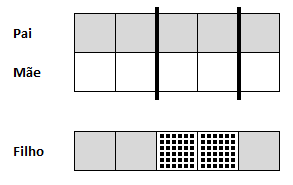
\includegraphics[width=.40\textwidth]{figs/materiais_metodo/software/pai-mae-filho-com-crossover.png} &
    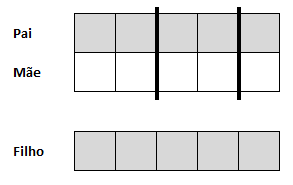
\includegraphics[width=.40\textwidth]{figs/materiais_metodo/software/pai-mae-filho-sem-crossover.png}
  \end{tabular}
  \caption{Diagrama do \emph{crossover} implementado. Na esquerda: \emph{crossover} acontece; na direita: \emph{crossover} acontece.}
	\label{fig:crossover_programa}
	\end{figure}

\vspace{1 cm}
\begin{lstlisting}
//============================================
void CrossOver2Pontos_serial(
  struct generation *g0,
  struct generation *g1,
  struct parametros *parametrosGA) {
//============================================

unsigned short int iIndividuo, idx_Pai, idx_Mae;
unsigned long int iGene;

struct individual *Pai, *Mae;
double f, p_aux;

for (iIndividuo = 0; iIndividuo < parametrosGA->numIndividuos; iIndividuo = iIndividuo + 1) {	

  idx_Pai = Randomico_int(0, parametrosGA->numIndividuos - 1);
  idx_Mae = Randomico_int(0, parametrosGA->numIndividuos - 1);

  Pai = &g0->individuo[idx_Pai];
  Mae = &g0->individuo[idx_Mae];

  p_aux = (double)((double)rand() / (double)RAND_MAX);

  f = -1.0F;

  g1->individuo[iIndividuo].pontos_de_corte[0] = Randomico_int(0, (parametrosGA->numGenes-1));
  g1->individuo[iIndividuo].pontos_de_corte[1] = Randomico_int(g1->individuo[iIndividuo].pontos_de_corte[0], (parametrosGA->numGenes-1));

  if (p_aux <= parametrosGA->probCrossOver) {

    f = (double)((double)rand()/(double)RAND_MAX);

    for (iGene = 0; iGene < g1->individuo[iIndividuo].pontos_de_corte[0]; iGene++) {
      g1->individuo[iIndividuo].gene[iGene] = Pai->gene[iGene];				
    }

    for (iGene = g1->individuo[iIndividuo].pontos_de_corte[0]; iGene < g1->individuo[iIndividuo].pontos_de_corte[1]; iGene++) {				
      g1->individuo[iIndividuo].gene[iGene] = f*Pai->gene[iGene] + (1 - f)*Mae->gene[iGene];				
    }

    for (iGene = g1->individuo[iIndividuo].pontos_de_corte[1]; iGene < parametrosGA->numGenes; iGene++) {
      g1->individuo[iIndividuo].gene[iGene] = Pai->gene[iGene];				
    }
  }
	
  else {
	
    for (iGene = 0; iGene < parametrosGA->numGenes; iGene++) {
      g1->individuo[iIndividuo].gene[iGene] =	g0->individuo[iIndividuo].gene[iGene];			
    }
  }
}
}
\end{lstlisting}
\vspace{1 cm}


%---------------------------------------------------
\subsection{Mutação}
%---------------------------------------------------

	Está no arquivo \textbf{\texttt{GA\_serial.h}}.
	
	Todos os genes de cada indivíduo estão sujeitos à mutação (laços das linhas 14 e 16). A condição de ocorrência é semelhante à do \emph{crossover}. Se uma probabilidade auxiliar, obtida aleatoriamente na linha 18, for menor que a problabilidade de mutação, o gene é alterado na linhas linhas 25--27 conforme equação \ref{eq:mutacao}. Os parâmetros necessários são obtidos nas linhas 21--23.
	
\vspace{1 cm}
\begin{lstlisting}
//============================================
void Mutacao_Serial(
  struct generation *geracao,
  struct parametros *parametrosGA) {
//============================================

unsigned short int iIndividuo;
unsigned long iGene;
unsigned short int L;
int termo_do_L;
double r, pAux;
double intensidadeMutacao = 10*geracao->Maior_fitness;

for (iIndividuo = 0; iIndividuo < parametrosGA->numIndividuos; iIndividuo++) {

  for (iGene = 0; iGene < parametrosGA->numGenes; iGene++) {

    pAux = (double)((double)rand() / (double)RAND_MAX);

    if (pAux <= parametrosGA->probMutacao) {
      L = Randomico_int(0, 10);
      r = (double)((double)rand() / (double)RAND_MAX) + 0.000002;
      termo_do_L = (int)pow((double)(-1),(int)L);
			
      geracao->individuo[iIndividuo].gene[iGene] =
          geracao->individuo[iIndividuo].gene[iGene] +
          (double)(termo_do_L * r * intensidadeMutacao);
    }
  }
}
}
\end{lstlisting}
\vspace{1 cm}


%---------------------------------------------------
\subsection{Fluxo principal}
%---------------------------------------------------
	
	Abaixo listo o código, presente no arquivo \textbf{\texttt{Serial\_novo.c}}, referente ao fluxo principal do GA (figura \ref{fig:fluxo}). Os operadores são aplicados na ordem: \emph{Fitness} (linha 7), Seleção (linha 44), \emph{Crossover} (linha 55) e Mutação (linha 66).
	
	O programa termina quando atinge o número máximo de gerações, testado na condição do \texttt{while} da linha 2, ou quando algum dos critérios de parada de precisão é atingido (linhas 37--40), definidos pelas equações \ref{eq:criterioParada024} e \ref{eq:criterioParada13}. Note que elas são testados logo após o \emph{fitness}, afinal, se uma geração contém boas soluções, não deve ser alterada pelos outros operadores genéticos.

\vspace{1 cm}
\begin{lstlisting}
//============================================
while (iGeracao < parmsPrograma.parmQtdeMaxGeracoes) {

  // FITNESS
  time_i = clock();
	
  Fitness_Serial(
    parmTipoFitnessEquacao,
    TipoCalculoGradRho,
    geracao0,
    &parametrosGA,
    &parametrosMetodo,
    Hamiltoniano,
    parametrosGA.numGenes,
    parametrosMetodo.lambda,
    parametrosMetodo.rho_minimo,
    MatrizIdentidade
  );
	
  time_f = clock();

  if (flagImprimeTempo == 1) {
    imprimeTempo(
      1, 0, 0, iGeracao, 4, 2, time_i, time_f,
      &parametrosGA, &parametrosMetodo, &parmsPrograma
    );
  }

  if (flagImprimeComportamentoFitness == 1) {
    imprimeComportamentoFitness(
      1, codMaquina, tipoPrograma, 0, iGeracao, geracao0,
      &parametrosMetodo, &parametrosGA, &parmsPrograma
    );
  }

  // CRITERIOS DE PARADA
  flagAtingiuTolerancia = atingiuCriterioDeParada(parmTipoFitnessEquacao, tolerancia, geracao0);
	
  if (flagAtingiuTolerancia == 1)
    break;

  // SELECAO
  time_i = clock();
  Selecao_Por_Torneio_serial(geracao0, geracao1, &parametrosGA);
  time_f = clock();
  if (flagImprimeTempo == 1) {
    imprimeTempo(
      1, 0, 0, iGeracao, 5, 2, time_i, time_f,
      &parametrosGA, &parametrosMetodo, &parmsPrograma
    );
  }

  // CROSSOVER
  time_i = clock();
  CrossOver2Pontos_serial(geracao1, geracao0, &parametrosGA);
  time_f = clock();
  if (flagImprimeTempo == 1) {
    imprimeTempo(
      1, 0, 0, iGeracao, 6, 2, time_i, time_f,
      &parametrosGA, &parametrosMetodo, &parmsPrograma
    );
}

  // MUTACAO
  time_i = clock();
  Mutacao_Serial(geracao0, &parametrosGA);
  time_f = clock();
  if (flagImprimeTempo == 1) {
    imprimeTempo(
      1, 0, 0, iGeracao, 7, 2, time_i, time_f,
      &parametrosGA, &parametrosMetodo, &parmsPrograma
    );
  }

  iGeracao++;
}
\end{lstlisting}
\vspace{1 cm}	
\chapter{Resultados e discussão}
\label{cap:resultados}

\begin{enumerate}
	
	\item Parágrafo de introdução do capítulo. Citar que, basicmente, o leitor encontrará no capítulo:
		\begin{enumerate}
			\item Resultados do ONEMAX, legitimando o uso do código para o programa mais complexo que foi utilizado no método dos indianos.
			\item o estudo dos tipos de \textit{fitness}, operador responsável pelo elo entre o algoritmo e o problema \cite{Linden2008}, que, para o nosso caso, é encontrar autovalores. Ponte para o próximo: para cada tipo de \textit{fitness}, um resultado diferente.
		\end{enumerate}

	\item Os dois tipos de fitness dos indianos. Ideia central: dois tipos, resultados diferentes. Com $\nabla \rho$ chegamos a um autovalor qualquer, com $(\rho - \rho_0)^2$ podemos chegar ao mínimo, mas dá mais trabalho. Ponte para o próximo: proposta de dois novos fitness.
	
	\item Combinação de $\nabla \rho$ com $(\rho - \rho_0)^2$. Se cada forma leva a comportamentos diferentes, tentamos combinar os dois termos em um único fitness. Uma hipótese seria a melhoria da qualidade dos resultados. A hipótese não foi confirmada. Ponte para o próximo: a busca pela qualidade levou à verificação da importância do parâmetro $\lambda$.
	
	\item Além do que os indianos disseram, que $\lambda$ é escolhido para não estourar a função exponencial, ele tem influência na convergência do algoritmo e na precisão (ou resolução) do fitness. Se na primeira população, geração inicial, o fitness médio é alto, isso provoca convergência precoce, fazendo com que o resultado final seja ruim. Por outro lado, se no início o fitness médio é muito baixo, não há muita discriminação entre os indivíduos, o fitness não cresce e não chegamos a uma solução. A medida que o fitness se aproxima de 1, a discriminação entre os indivíduos fica difícil, levando ao problema da resolução. Ponte para o próximo: vários testes levaram ao desenvolvimento de uma equação empírica para $\lambda$, restrita às matrizes de Coope$-$Sabo \cite{Coope1977}.
	
	\item Fórmula empírica. Por já conhecermos de antemão os autovalores das matrizes de Coope$-$Sabo, foi possível criar uma fórmula empírica para $\lambda$. Ela garante que na primeira população o \textsl{fitness} médio é baixo, previnindo o \textsl{underflow} do \textit{fitness} e a convergência prematura.
	
	\end{enumerate}
	
\section{Problemas com o mínimo global}	
	
	Na seção \ref{sec:metodo} vimos que o \textit{fitness} utilizado no artigo \cite{metodo2004}  foi
	
	\begin{equation}
		\label{eq:fitnessGrad2}
		f_i = e^{-\lambda \| \nabla \rho_i \|^2},
	\end{equation}
	onde $f_i$ é o \textit{fitness} do $i$-ésimo indivíduo da população, $\lambda$ é um parâmetro para evitar o estouro do \textit{fitness} e $\| \nabla \rho_i\|^2$ é o módulo ao quadrado do vetor gradiente de $\rho$, dado por
		
				\begin{equation}
					\nabla \rho_i = \frac{2[H - \rho_i]C_i}{C_i^t C_i},
				\end{equation}
	em que $C_i$ é um vetor candidato à solução do problema do autovalor
	
	\begin{equation}
		HC = EC.
	\end{equation}
	
	Além disso, se $C_i$ é de fato um dos autovetores, $\rho$ é o autovalor associado $E_i$:
	
	\begin{equation}\label{eq:rho_eh_E}
		\rho_i = \frac{C_i^t H C_i}{C_i^t C_i} = E_i.
	\end{equation}
	
	A fim de reproduzir os resultados, testamos o método com matrizes de Coope\-Sabo de ordem 10, 20, 30 e 40, utilizando os mesmos parâmetros encontrados em \cite{metodo2004}: probabilidade de \textit{crossover} $p_c = 75\%$, probabilidade de mutação $p_m = 50\%$ e intensidade de mutação $\Delta = 0,01$. Com um bom ajuste de $\lambda$, que será discutido em detalhes posteriormente, o \textit{fitness} comportou-se conforme o esperado em todos os casos. Um exemplo está na figura \ref{fig:compFitnessTipo1N10}, que apresenta o melhor fitness de cada geração para uma matriz de ordem N = 10. Na primeira geração o melhor \textit{fitness} é pequeno, aproximadamente 0,1, cresce rapidamente e a partir da décima geração está próximo de 1.
	
	\begin{figure}[htbp]
		\centering
			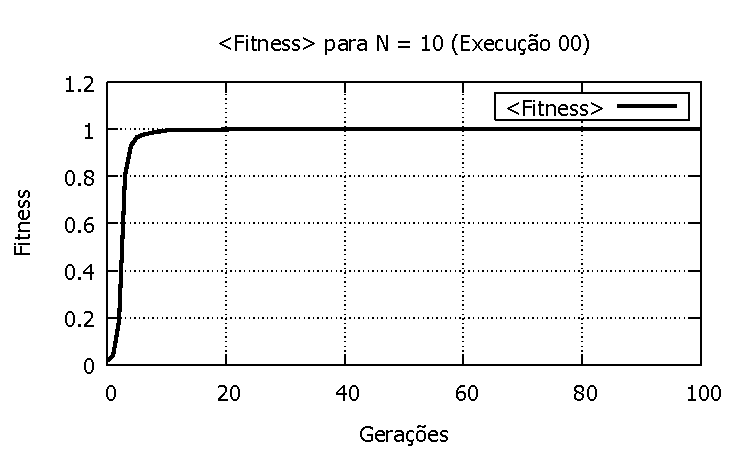
\includegraphics{figs/resultados/fitnessGrad/N10_00_fitness.pdf}
			\caption{Comportamento do \textsl{fitness} $f_i = e^{-\lambda \| \nabla \rho_i \|^2}$ para N = 10. Na primeira geração o melhor \textit{fitness} é pequeno, aproximadamente 0,1, cresce rapidamente e a partir da décima geração está próximo de 1.}
		\label{fig:compFitnessTipo1N10}
	\end{figure}
	
	O próximo passo foi verificar o comportamento de $\rho$, o Quociente de Rayleigh, e, especificamente, sua convergência para o menor autovalor $E_0$. Ainda conforme \cite{metodo2004}, obteríamos uma curva semelhante à da figura \ref{fig:compFitnessTipo1N10}, mas invertida, ou seja, os primeiros valores de $\rho$ seriam grandes e, rapidamente, diminuiriam até haver convergência para o autovalor mínimo. Na figura \ref{fig:rho_N10} há um exemplo.	Os gráficos exibem os valores de $\rho$ para a mesma execução apresentada na figura \ref{fig:compFitnessTipo1N10}. Note no primeiro gráfico que até a geração 20 o quociente $\rho$ teve caráter oscilatório e, então, aparentemente estabilizou-se entre 6 e 8, valores muito superiores ao autovalor mínimo para essa matriz, $E_0 = 0,38675$. Entretanto, ainda no primeiro gráfico, observa-se que há uma tendência de queda do $\rho$ entre as gerações 40 e 50 e, portanto, existiria a possibilidade do algoritmo convergir para $E_0$. Porém, para esse exemplo especificamente, isso não aconteceu, como pode ser visto no segundo gráfico da figura \ref{fig:rho_N10}. Para garantir a estabilidade, o programa foi executado até a geração 400.000, e o valor médio obtido foi $<\rho> = 6,572898$. Para nossa surpresa, além do valor obtido de $<\rho>$ não ser o mínimo, ele não é um valor qualquer, mas corresponde, com erro menor que $0,00002\%$, ao quarto autovalor da matriz, $E_3 = 6,572897$. Um gráfico expandido dessa execução está na figura \ref{fig:rho_N10_completa} da página \pageref{fig:rho_N10_completa}. Pensamos, então, que poderia haver algo de errado com o nosso programa. 
	
	\begin{figure}[htbp]
		\centering
			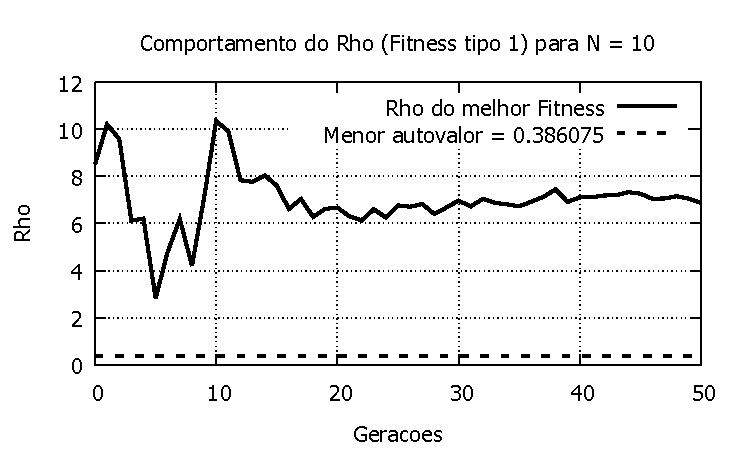
\includegraphics[width=0.40\textwidth]{figs/resultados/rho_N10_g50.pdf}
			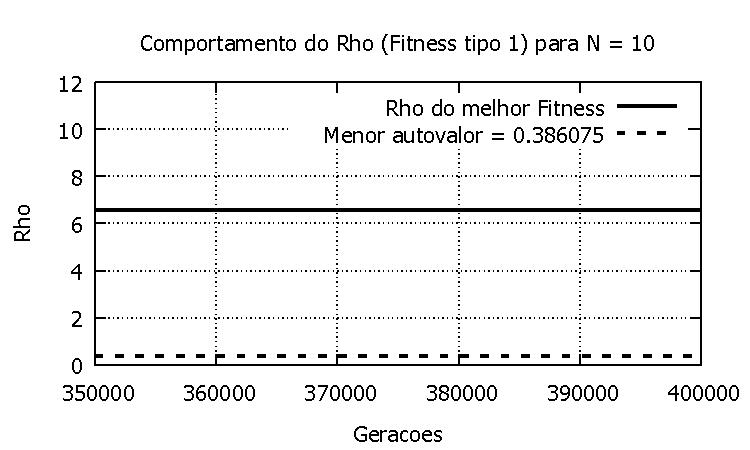
\includegraphics[width=0.40\textwidth]{figs/resultados/rho_N10_g400000.pdf}
		\caption{Comportamento de $\rho$ (Quociente de Rayleigh) para uma matriz de Coope$-$Sabo de ordem 10.}
		\label{fig:rho_N10}
	\end{figure}
	
	\newpage
	\begin{landscape}
	\begin{figure}[p]
		\centering
			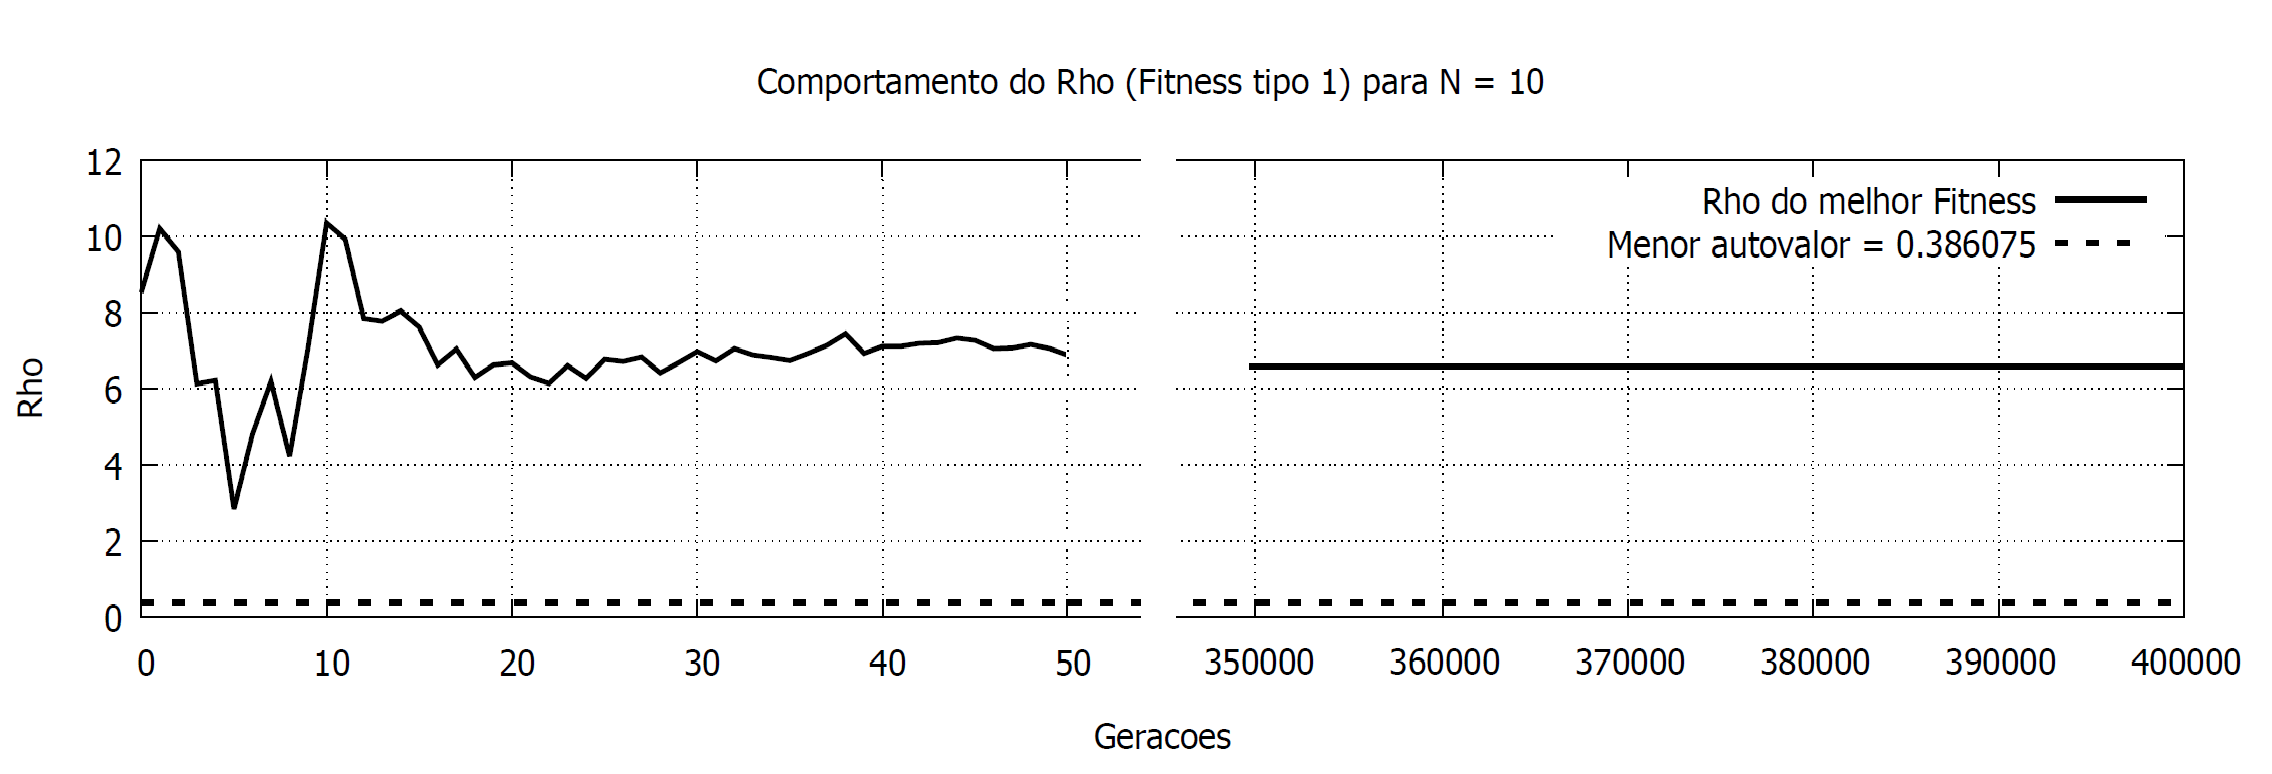
\includegraphics[width=1.3\textwidth]{figs/resultados/rho_N10.png}
		\caption{Comportamento de $\rho$ (Quociente de Rayleigh) para uma matriz de Coope$-$Sabo de ordem 10.}
		\label{fig:rho_N10_completa}
	\end{figure}
	\end{landscape}
	\newpage
			
	Após esses resultados preliminares executamos uma validação cuidadosa do programa, testando cada uma de suas quase 2500 linhas e comparando os resultados das operações e cálculos com os softwares Excel \cite{excel} e SciLab \cite{scilab}. A hipótese era a de que erros numéricos, principalmente nas funções de álgebra linear e nos operadores genéticos, pudessem ter levado ao comportamento incorreto da não convergência para o menor autovalor. De fato alguns erros foram encontrados.
	
	Discutiremos a seguir os testes com a versão corrigida do programa e exibidos nas figuras \ref{fig:execucoes_N10}, \ref{fig:execucoes_N20}, \ref{fig:execucoes_N30} e \ref{fig:execucoes_N40}. Visando brevidade, apresentaremos dados para matrizes de Coope\-Sabo de ordem 10, 20, 30 e 40 apenas, sem perda de generalidade. Foram cinco execuções para cada matriz, até a geração 400.000, gerando sempre dois gráficos, um do \textit{fitness} médio (<\textit{fitness}>) e outro do Quociente de Rayleigh médio (<$\rho$>), ambos em função do número de gerações, e dando ênfase às primeiras 100 gerações. Essas escolhas, número máximo da geração e uso de médias sobre cada população, visaram garantir, respectivamente, a convergência genética e boa precisão. A exibição de apenas as primeiras 100 gerações tem como objetivo olhar em detalhe (com \textit{zoom}) o período em que o \textit{crossover} tem mais peso, ou seja, onde há geralmente os saltos no espaço de soluções de um Algoritmo Genético. Em todos os gráficos de $<\rho>$ há indicado nas legendas o autovalor mínimo $E_0$ e o autovalor obtido após as 400.000 gerações ($E_{obtido}$). Na tabela \ref{tab:autovalores10a40} há a lista de todos os autovalores. Por exemplo, para uma matriz de ordem $N = 10$, o menor autovalor é $E_0 = $0,386075, e o quinto autovalor para $N = 30$ é $E_4$ = 8,450274.
	
	Comecemos a discussão com o que foi encontrado em todas as execuções. Em qualquer gráfico do \textit{fitness} observa-se estabilidade do comportamento conforme esperado pelo método: no início seu valor é baixo, próximo de zero, cresce rapidamente nas primeiras gerações e fica estável próximo de $<fitness> = 1$. Com relação ao $\rho$, há sempre oscilações, sejam pequenas variações em torno de uma clara linha de tendência, como na execução 02 para N = 10, ou grandes saltos, como nas execuções 05 de N = 20 e 05 de N = 30. Novamente, o menor autovalor não foi obtido em nenhuma execução, contradizendo os resultados de \cite{metodo2004}, mas, por outro lado, o algoritmo sempre encontrou algum autovalor.
	
	De fato, verificando os dados da tabela \ref{tab:execucoes10a40}, concluímos que tais valores não devem ser coincidência. Para todas as execuções o \textit{fitness} médio chegou ao valor máximo ($<f> = 1,000000$). As médias de $\rho$ sobre todos os indivíduos da última população possuem baixo desvio padrão ($\sigma$ < 0,0001), indicando que eles são muito parecidos entre si e que o algoritmo atingiu a convergência genética. Ou seja, não há variabilidade genética suficiente na população para alterar o rumo da busca de modo a atingir o menor autovalor, ou o mínimo global. Portanto, o algoritmo chegou em um mínimo local, corroborado pelos baixos erros relativos de $<\rho>$ quando comparado com o autovalor mais próximo. Por exemplo, para N = 30, execução 4,  $<\rho>$ = 40,772447, correspondendo, com erro relativo absoluno menor que $0,001\%$, ao vigésimo primeiro autovalor, $E_{20} = 40,772850$. Apesar das evidências descritas acima, até esse ponto ainda há dúvidas sobre a validade do nosso programa e, obviamente, dos resultados produzidos. Então, buscamos embasamento mais rigoroso.

De acordo com \cite{metodo2004}, se algum $C_i$, em algum momento, é o autovetor fundamental (associado ao menor autovalor), o $\nabla \rho$ é nulo. Com o \textit{fitness} da equação \eqref{eq:fitnessGrad2} os autores afirmam que ``\textit{Claramente, $f_i \rightarrow 1$ quando $\nabla \rho_i \rightarrow 0$, sinalizando que a evolução atingiu o verdadeiro autovetor fundamental de $H$ em $C_i$}''\footnote{Tradução livre de ``\textit{Clearly, $f_i \rightarrow 1$, as $\nabla \rho_i \rightarrow 0$, signalling that the evolution has hit the true ground state eigenvector of $H$ in the vector $C_i$}''.}. Há duas relações distintas de causalidade nessa frase, e acreditamos que nelas residam a explicação dos resultados obtidos por nós até agora.

A primeira relação de causalidade refere-se à afirmação ``\textit{$f_i \rightarrow 1$ quando $\nabla \rho_i \rightarrow 0$}'', que está absolutamente correta. Retomando a seção \ref{cap:metodologia}, o \textit{fitness} definido pela equação \ref{eq:fitnessGrad2} é limitado no intervalo (0,1] e, como $\lambda > 0$, só chega ao seu valor máximo quando $\nabla \rho_i = 0$. Em outras palavras, $\nabla \rho_i \rightarrow 0$ implica $f_i \rightarrow 1$.

Na afirmação ``(...) \textit{sinalizando que a evolução atingiu o verdadeiro autovetor fundamental de $H$ em $C_i$}'' reside a segunda relação de causalidade que, apesar de sutil, é muito poderosa:

\begin{equation}\label{eq:afirmacaoErrada}
	\mbox{Se } f_i \rightarrow 1\mbox{, } C_i = C_0.
\end{equation}

Ou seja, sempre que algum indivíduo $C_i$, de qualquer população, possuir \textit{fitness} muito próximo de 1, isso implica que, além de ter uma excelente ``nota'', ele, ainda por cima, é um vetor especial, o autovetor fundamental $C_0$. Portanto, possui autovalor associado $E_0$, o autovalor mínimo (conforme equação \ref{eq:rho_eh_E}). Grosso modo, $f_i(C_i) = 1$ implica que $C_i = C_0$ e que podemos obter $E_0(C_0)$:

\begin{equation}\label{eq:causalidadeErrada}
	f_i(C_i) = 1 \rightarrow C_i = C_0 \rightarrow E_0(C_0).
\end{equation}

As relações de causa e efeito da equação acima estão erradas. Em sua obra clássica sobre o problema de autovalores em matrizes simétricas, \cite{Parlett1998} abre o capítulo introdutório frisando que ``\textit{em muitos lugares no livro, é feita referência a fatos mais ou menos bem conhecidos sobre a teoria de matrizes}''\footnote{Tradução livre de ``\textit{At many places in the book, reference is made to more or less well known facts from matrix theory}''.}. Conforme já dito no capítulo \ref{cap:algebra}, um desses fatos diz que $\rho(\mbox{\textit{u}})$ é estacionário, ou seja, $\nabla \rho(\mbox{\textit{u}}) = 0$, apenas se o vetor \textit{u} é um autovetor $w$ de $HC = EC$. Consequentemente, o encadeamento correto se apresenta como:

\begin{equation}\label{eq:causalidadeCorreta}
	C_i \mbox{ é um autovetor} \rightarrow \nabla \rho(C_i) = 0 \rightarrow f_i = 1.
\end{equation}
	
Então, se $f_i = 1$, o máximo que podemos concluir é que $C_i$ é \textit{algum} autovetor, e não necessariamente \textit{o} autovetor fundamental. Ao fim de todos os nossos testes o \textit{fitness} médio foi <\textit{f}> = 1, a população final era composta por autovetores e foi possível, com boa precisão, obter os autovalores relacionados (não necessariamente o autovalor mínimo). Nossos dados confirmam a matemática e, assim, acreditamos que nosso programa não contém erros.

Apesar de não chegar ao mínimo, o método pode ser utilizado de maneira exploratória com relativa facilidade, bastando extrair $\rho$ sempre que $f_i \rightarrow 1$ e $\nabla \rho \rightarrow 0$. 

Resta a dúvida: afinal, como o autovalor mínimo foi obtido com o \textit{fitness} definido pela equação \ref{eq:fitnessGrad2}? Não sabemos. Esse \textit{fitness} foi utilizado não só em \cite{metodo2004}, mas também em \cite{metodo2006}, \cite{metodo2008} e \cite{metodo2009}, seguindo exatamente o argumento resumido pela equação \ref{eq:causalidadeErrada}. Não identificamos nada nesses quatro artigos que pudesse levar à resposta. Seguimos o estudo com uma nova definição do \textit{fitness} encontrada em \cite{metodo2011}.

\begin{landscape}
\begin{center}
\begin{table}[htbp]
\caption{Execuções para matrizes de Coope$-$Sabo.}
\label{tab:execucoes10a40}
% Table generated by Excel2LaTeX from sheet 'Plan1 (2)'
\begin{tabular}{cccccccccc}
\hline \hline
   \textbf{N} & \textbf{Execução} & \textbf{Semente} & \textbf{$\lambda$} & \textbf{<\textit{Fitness}>} & \textbf{<$\rho$>} & \textbf{$\sigma$} & \textbf{\# autovalor} & \textbf{Autovalor} & \textbf{Erro relativo} \\
\hline \hline
        10 &          0 & 1445738835 &   0,128788 &   1,000000 &   2,461122 &   0,000023 &          1 &   2,461056 &    0,003\% \\
\hline
        10 &          1 & 1445780626 &   0,128788 &   1,000000 &   6,572898 &   0,000013 &          3 &   6,572897 &  0,00001\% \\
\hline
        10 &          2 & 1445780762 &   0,128788 &   1,000000 &   6,572883 &   0,000015 &          3 &   6,572897 &  -0,0002\% \\
\hline
        10 &          3 & 1445780907 &   0,128788 &   1,000000 &   6,572910 &   0,000016 &          3 &   6,572897 &   0,0002\% \\
\hline
        10 &          4 & 1445781049 &   0,128788 &   1,000000 &  12,765701 &   0,000016 &          6 &  12,765740 &  -0,0003\% \\
\hline
        10 &          5 & 1445781195 &   0,128788 &   1,000000 &   4,518952 &   0,000012 &          2 &   4,518931 &   0,0005\% \\
\hline
        20 &          1 & 1445795292 &   0,026665 &   1,000000 &   8,498192 &   0,000052 &          4 &   8,497626 &    0,007\% \\
\hline
        20 &          2 & 1445795501 &   0,026665 &   1,000000 &  12,551830 &   0,000018 &          6 &  12,551780 &   0,0004\% \\
\hline
        20 &          3 & 1445795718 &   0,026665 &   1,000000 &  12,551878 &   0,000020 &          6 &  12,551780 &   0,0008\% \\
\hline
        20 &          4 & 1445795953 &   0,026665 &   1,000000 &  14,578527 &   0,000035 &          7 &  14,578450 &   0,0005\% \\
\hline
        20 &          5 & 1445796166 &   0,026665 &   1,000000 &  18,634220 &   0,000062 &          9 &  18,633850 &    0,002\% \\
\hline
        30 &          1 & 1445796378 &   0,011171 &   1,000000 &  26,616790 &   0,000065 &         13 &  26,616670 &   0,0005\% \\
\hline
        30 &          2 & 1445796746 &   0,011171 &   1,000000 &  26,616595 &   0,000029 &         13 &  26,616670 &  -0,0003\% \\
\hline
        30 &          3 & 1445797109 &   0,011171 &   1,000000 &  22,580060 &   0,000051 &         11 &  22,580300 &   -0,001\% \\
\hline
        30 &          4 & 1445797473 &   0,011171 &   1,000000 &  40,772447 &   0,000071 &         20 &  40,772850 &   -0,001\% \\
\hline
        30 &          5 & 1445797882 &   0,011171 &   1,000000 &  30,655283 &   0,000022 &         15 &  30,655270 &  0,00004\% \\
\hline
        40 &          1 & 1445798248 &   0,006105 &   1,000000 &  26,554758 &   0,000040 &         13 &  26,554690 &   0,0003\% \\
\hline
        40 &          2 & 1445798838 &   0,006105 &   1,000000 &  54,773734 &   0,000078 &         27 &  54,773690 &  0,00008\% \\
\hline
        40 &          3 & 1445799429 &   0,006105 &   1,000000 &  58,819413 &   0,000087 &         29 &  58,819810 &  -0,0007\% \\
\hline
        40 &          4 & 1445800091 &   0,006105 &   1,000000 &  40,651473 &   0,000077 &         20 &  40,651140 &   0,0008\% \\
\hline
        40 &          5 & 1445800683 &   0,006105 &   1,000000 &  40,650764 &   0,000061 &         20 &  40,651140 &  -0,0009\% \\
\hline \hline
\end{tabular}
\end{table}  
\end{center}
\end{landscape}

\section{Outro \textit{fitness} para encontrar o mínimo global}

	O novo \textit{fitness}, apresentado em \cite{metodo2011}, é dado por
	
	\begin{equation}\label{eq:fitnessRho0}
		f_i = e^{-\lambda(\rho_i - E_L)^2},
	\end{equation}
e apresenta semelhanças com o definido pela equação \ref{eq:fitnessGrad2}. Há uso de uma exponencial, o parâmetro $\lambda$ foi mantido e possui exatamente o mesmo papel, $f_i$ depende apenas de $\rho$ e, como $(\rho_i - E_L)^2$ é claramente positivo, o \textit{fitness} continua limitado ao conjunto (0,1]. As diferenças estão na ausência do $\nabla \rho$ e na inclusão do parâmetro $E_L$, que representa um limite inferior para o \textit{menor} autovalor que estamos procurando\footnote{L de \textit{lower}.}. Por exemplo, se soubermos de antemão que o autovalor \textit{mínimo} é maior que zero, poderíamos definir $E_L = 0$. 

	 A justificativa para o funcionamento do método em \cite{metodo2011} segue a mesma estrutura de \cite{metodo2004}: ``\textit{Se $\rho_i \rightarrow E_L$ durante a busca, $f_i \rightarrow 1$ e $C_i$ está próximo do autovetor fundamental de $H$}''\footnote{Tradução minha para ``\textit{If $\rho_i \rightarrow E_L$ during the search, $f_i \rightarrow 1$ and $C_i$ approaches the ground eigenvector of $H$}''.}. Parece que, outra vez, não há garantia de que, se $f_i \rightarrow 1$, $\rho$ tende, necessariamente, ao autovalor fundamental. E aqui há um agravante: nada na equação \ref{eq:fitnessRho0} está diretamente associado aos autovalores de $H$. Lembre-se que o \textit{fitness} anterior (equação \ref{eq:fitnessGrad2}) contém $\nabla \rho$, que possui relação direta com os autovalores de $H$ quando $\nabla \rho = 0$.
	
	Repeti as execuções da tabela \ref{tab:execucoes10a40} alterando apenas o \textit{fitness} e configurando o parâmetro $E_L$ para $E_L = 0$, um pouco abaixo dos autovalores mínimos. Os resultados estão na página \pageref{tab:execucoesNovoFitness}, e os gráficos da evolução do \textit{fitness} e do quociente de Rayleigh estão nas páginas \pageref{fig:execucoes_N10_EL}, \pageref{fig:execucoes_N20_EL}, \pageref{fig:execucoes_N30_EL} e \pageref{fig:execucoes_N40_EL}. Surpreendentemente, apesar do que foi dito no parágrafo anterior, o programa encontrou o menor autovalor em \textbf{todos} os casos. Assim como nas primeiras execuções, o desvio padrão ($\sigma$) da média de $\rho$ na última geração (400.000) foi pequeno, indicando convergência genética. Entretanto, essa foi a única semelhança. Os próprios valores de $\sigma$ são uma ordem de grandeza menores, sugerindo que os indivíduos são mais semelhantes entre si. O \textit{fitness} médio só atingiu seu valor máximo para a matriz de ordem $N = 40$. Aliás, especificamente para $E_L$ fixado em $E_L = 0$, o <\textit{fitness}> final diminui com $N$, pois $E_L$ está mais distante de $E_0$ na matriz de ordem 10 do que na de ordem 40. Os erros relativos não ultrapassaram $1\%$, mas foram substancialmente maiores comparados aos obtidos com o primeiro \textit{fitness}. Enquanto nos testes anteriores seus valores permaneceram estáveis, agora os erros relativos apresentaram tendência de crescimento com N.
	
	\begin{landscape}
\begin{center}
\begin{table}[htbp]
\caption{Execuções novo \textit{Fitness}.}
\label{tab:execucoesNovoFitness}
	% Table generated by Excel2LaTeX from sheet 'Tabela LaTex'
\begin{tabular}{cccccccccc}
\hline \hline
   \textbf{N} & \textbf{Execução} & \textbf{Semente} & \textbf{$\lambda$} & \textbf{<Fitness>} & \textbf{<$\rho$>} & \textbf{$\sigma$} & \textbf{\# autovalor} & \textbf{Autovalor} & \textbf{Erro relativo (\%)} \\
\hline \hline
        10 &          0 & 1445738835 &   0,128788 &   0,999044 &   0,386176 &    0,00005 &          0 &  0,3860745 &     0,03\% \\
\hline
        10 &          1 & 1445780626 &   0,128788 &   0,999044 &   0,386169 &    0,00003 &          0 &  0,3860745 &     0,02\% \\
\hline
        10 &          2 & 1445780762 &   0,128788 &   0,999045 &   0,386132 &    0,00002 &          0 &  0,3860745 &     0,01\% \\
\hline
        10 &          3 & 1445780907 &   0,128788 &   0,999044 &   0,386175 &    0,00005 &          0 &  0,3860745 &     0,03\% \\
\hline
        10 &          4 & 1445781049 &   0,128788 &   0,999043 &   0,386211 &    0,00003 &          0 &  0,3860745 &     0,04\% \\
\hline
        10 &          5 & 1445781195 &   0,128788 &   0,999044 &   0,386183 &    0,00005 &          0 &  0,3860745 &     0,03\% \\
\hline
        20 &          1 & 1445795292 &   0,026665 &   0,999954 &   0,341484 &    0,00005 &          0 &  0,3412367 &     0,07\% \\
\hline
        20 &          2 & 1445795501 &   0,026665 &   0,999954 &   0,341693 &     0,0001 &          0 &  0,3412367 &      0,1\% \\
\hline
        20 &          3 & 1445795718 &   0,026665 &   0,999954 &    0,34147 &    0,00006 &          0 &  0,3412367 &     0,07\% \\
\hline
        20 &          4 & 1445795953 &   0,026665 &   0,999954 &   0,341689 &     0,0001 &          0 &  0,3412367 &      0,1\% \\
\hline
        20 &          5 & 1445796166 &   0,026665 &   0,999954 &    0,34153 &    0,00007 &          0 &  0,3412367 &     0,09\% \\
\hline
        30 &          1 & 1445796378 &   0,011171 &   0,999995 &   0,320582 &     0,0001 &          0 &   0,319737 &      0,3\% \\
\hline
        30 &          2 & 1445796746 &   0,011171 &   0,999995 &   0,320772 &     0,0002 &          0 &   0,319737 &      0,3\% \\
\hline
        30 &          3 & 1445797109 &   0,011171 &   0,999995 &   0,320699 &     0,0001 &          0 &   0,319737 &      0,3\% \\
\hline
        30 &          4 & 1445797473 &   0,011171 &   0,999995 &   0,320755 &     0,0001 &          0 &   0,319737 &      0,3\% \\
\hline
        30 &          5 & 1445797882 &   0,011171 &   0,999995 &   0,320274 &    0,00007 &          0 &   0,319737 &      0,2\% \\
\hline
        40 &          1 & 1445798248 &   0,006105 &          1 &   0,306968 &     0,0001 &          0 &   0,306086 &      0,3\% \\
\hline
        40 &          2 & 1445798838 &   0,006105 &          1 &   0,307128 &     0,0001 &          0 &   0,306086 &      0,3\% \\
\hline
        40 &          3 & 1445799429 &   0,006105 &          1 &   0,307297 &     0,0002 &          0 &   0,306086 &      0,4\% \\
\hline
        40 &          4 & 1445800091 &   0,006105 &          1 &   0,307816 &     0,0002 &          0 &   0,306086 &      0,6\% \\
\hline
        40 &          5 & 1445800683 &   0,006105 &          1 &    0,30765 &     0,0002 &          0 &   0,306086 &      0,5\% \\

\hline \hline
\end{tabular}
\end{table}  
\end{center}
\end{landscape}
	
	As diferenças dos valores finais são indiscutíveis, sugerindo que o comportamento do \textit{fitness} e do $\rho$ ao longo da busca também deve ter sido alterado. Na figura \ref{fig:N-10_E-0_fitness} estão os gráficos referentes à execução zero para o Hamiltoniano de ordem 10, semente 1445738835. A primeira usa o \textit{fitness} $f_i = e^{-\lambda(\rho_i - E_L)^2}$, que chega ao autovalor mínimo, enquanto a segunda utiliza o $f_i = e^{-\lambda \| \nabla \rho_i \|^2}$. Ambos saem de valores muito baixos e convergem para 1, entretanto, o da esquerda é muito ruidoso e, aparentemente, essa é a causa da convergência mais lenta. Quando a curva da direita já está estável em $\textit{<f>} \approx 1$ em torno da geração de número 15, a da esquerda ainda não ultrapassou o $\textit{<f>} = 0,1$. A princípio, não podemos comparar os dois comportamentos diretamente, visto que cada um chegou em um autovalor diferente. A execução da direita, lembre-se, obteve apenas um mínimo local ($E_1 = 2,461056$, tabela \ref{tab:execucoes10a40}).
	
	\begin{figure}[htbp]
		\centering
			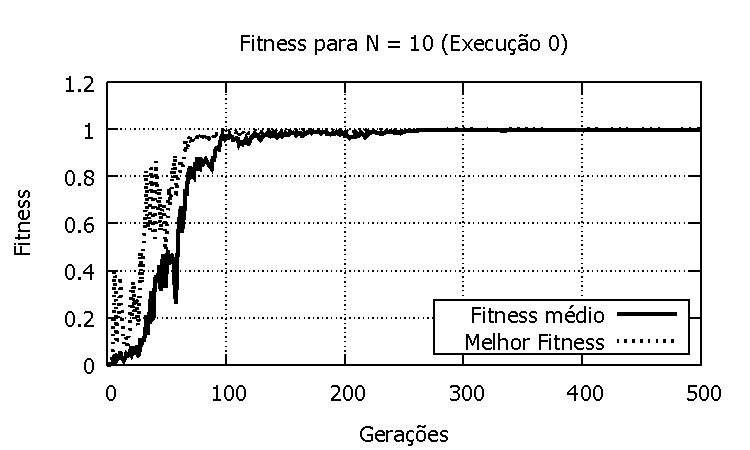
\includegraphics[width=0.48\textwidth]{figs/resultados/fitnessEL/N-10_E-0_fitness.pdf}
			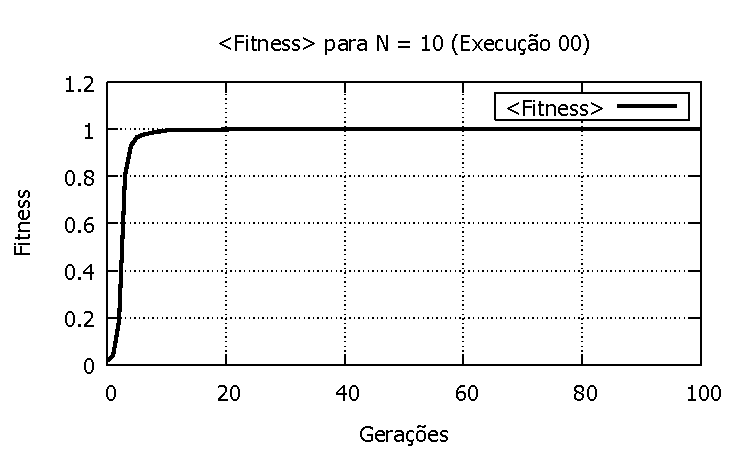
\includegraphics[width=0.48\textwidth]{figs/resultados/fitnessGrad/N10_00_fitness.pdf}
		\caption{Comportamento do \textit{fitness} para as execuções zero do Hamiltoniano de ordem 10, semente 1445738835. A primeira usa o \textit{fitness} $f_i = e^{-\lambda(\rho_i - E_L)^2}$, que chega ao autovalor mínimo, enquanto a segunda utiliza o $f_i = e^{-\lambda \| \nabla \rho_i \|^2}$.}
		\label{fig:N-10_E-0_fitness}
	\end{figure}
	
	De todo modo, as duas execuções estão conectadas pois, como partiram da mesma semente de números pseudoaleatórios, a população inicial foi \textit{exatamente} a mesma. Inclusive, na primeira geração, em ambas as execuções, os valores para $<\rho>$ e para o melhor $\rho$ foram, respectivamente, $9,876075$ e $9,557892$, igualmente distantes do autovalor mínimo $E_0 = 0,386075$. Os gráficos da figura \ref{fig:N-10_E-0_rho_comparacao} permitem comparar a evolução do $<\rho>$ nos dois casos. Assim como na figura anterior, a imagem da esquerda refere-se ao uso do \textit{fitness} $f_i = e^{-\lambda(\rho_i - E_L)^2}$.
	
	É tentador afirmar que a causa de uma execução ter sido mais lenta do que a outra foi porque percorreu um caminho mais longo ao sair de $<\rho> = 9,876075$, passar por $E_1 = 2,461056$ e continuar até encontrar $E_0 = 0,386075$, enquanto a mais rápida saiu do mesmo $<\rho>$ e parou logo que encontrou $E_1$. Infelizmente essa conclusão estaria incorreta. A maneira como os Algoritmos Genéticos viajam no espaço de soluções tem forte base estocástica e, portanto, qualquer comparação linear é extremamente arriscada, quiçá impossível. Objetivamente, posso apenas concluir que os valores finais encontrados por cada \textit{fitness} estão condizentes com a construção de cada função objetivo: $\nabla \rho_i$ leva a qualquer autovalor; $\rho_i - E_L$ encontra o autovalor mínimo.
	
	
	\begin{figure}[htbp]
		\centering
			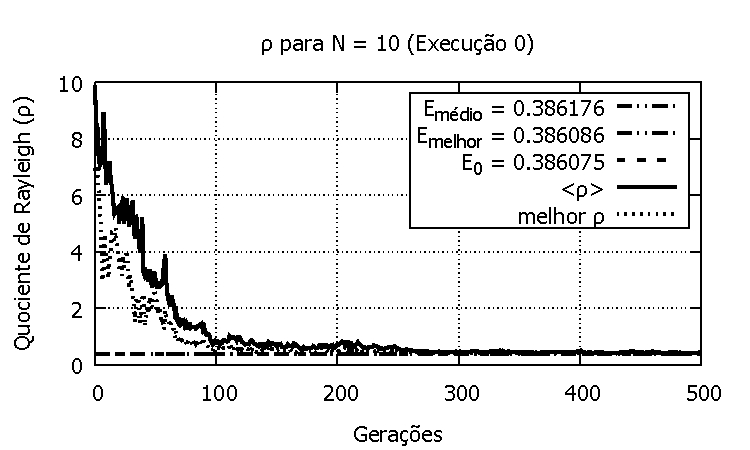
\includegraphics[width=0.48\textwidth]{figs/resultados/fitnessEL/N-10_E-0_rho.pdf}
			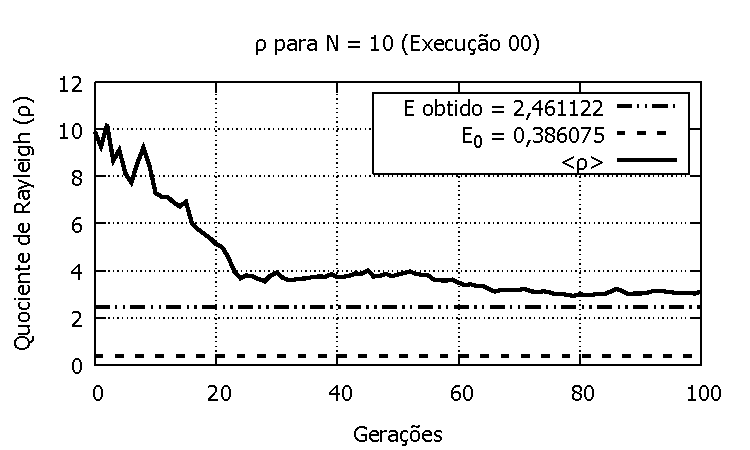
\includegraphics[width=0.48\textwidth]{figs/resultados/fitnessGrad/N10_00_rho.pdf}
		\caption{Comportamento do $\rho$ para as execuções zero do Hamiltoniano de ordem 10, semente 1445738835. A primeira usa o \textit{fitness} $f_i = e^{-\lambda(\rho_i - E_L)^2}$, que chega ao autovalor mínimo, enquanto a segunda utiliza o $f_i = e^{-\lambda \| \nabla \rho_i \|^2}$.}
		\label{fig:N-10_E-0_rho_comparacao}
	\end{figure}
	
	
	
		
	
	Ok. Os dados mostraram que chega no menor autovalor. Mas, se não há relação direta no fitness, como isso acontece? Outra sutileza: $E_L$ é um limite inferior para o \textit{menor} autovalor. Roubada? Não parece muito útil, pois o fitness só foi próximo de 1 porque escolhi um $E_L$ bem próximo de $E_0$. Mas, o que aconteceria se eu não soubesse por onde anda ou autovalor mínimo? Quatro cenários para $E_L$. Cenário 1: com sorte, o $E_L$ escolhido está um pouco abaixo do $E_0$. Encontra o valor mínimo, conforme exemplos. Cenário 2: um pouco acima de $E_0$. Cenário 3: muito abaixo de $E_0$; Cenário 4: muito acima de $E_0$.
	
	
	Semente 1445738835. Tipo 1. EL um pouco acima. Sempre converge para $E_L$. ``Passa'' por todos os autovalores, mas não para em nenhum. Aconteceu em \emph{todas} as execuções.
	
	\begin{figure}[htbp]
	\centering
  \begin{tabular}{@{}cc@{}}
	
		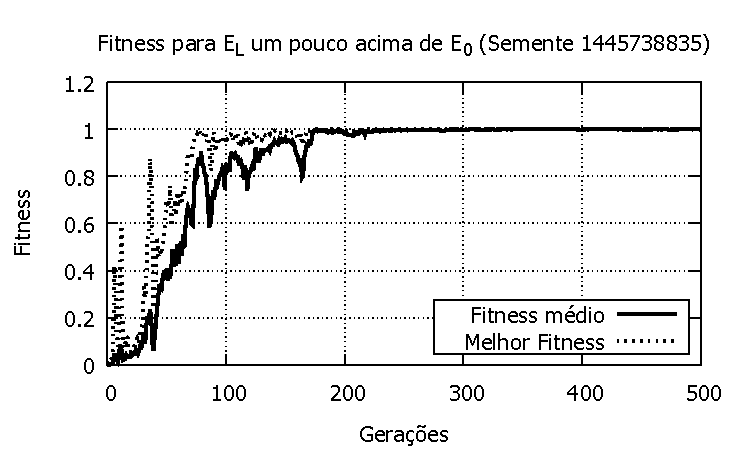
\includegraphics[width=.45\textwidth]{figs/resultados/variandoELSemente/T1_S-1445738835_fitness.pdf} &
    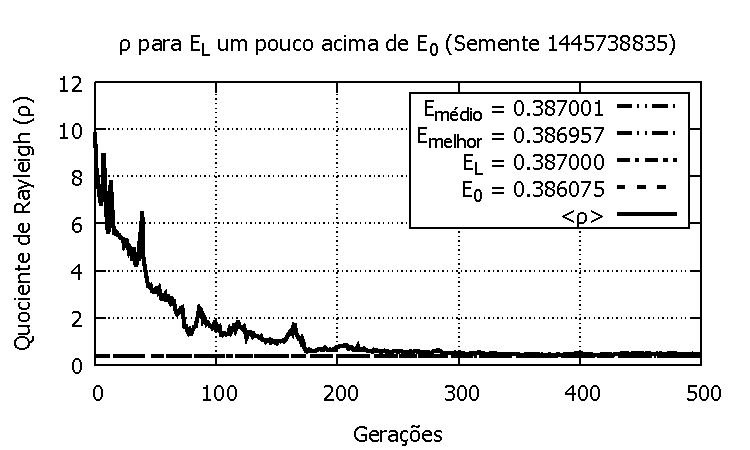
\includegraphics[width=.45\textwidth]{figs/resultados/variandoELSemente/T1_S-1445738835_rho.pdf}
  \end{tabular}
  \caption{Execução para a semente 1445738835. $E_L$ um pouco acima de $E_0$ no \textit{fitness} $f_i = e^{-\lambda(\rho_i - E_L)^2}$.}
	\label{fig:execucoesSemente_EL_umPoucoAcima}
	\end{figure}
	
	$E_L$ um pouco abaixo. Já citado no início da seção. Chegou ao menor autovalor em todas as execuções. \emph{Fitness} médio é próximo de 1 pois $E_L$ está próximo de $E_0$. Melhor cenário.
	
	Semente 1445738835. Tipo 3. $E_L$ muito acima. Novamente, chegou ao $E_L$ em todas as execuções. Tendo cuidado com o $\lambda$, parece não haver diferenças entre \emph{um pouco} acima e \emph{muito} acima. Mas, aqui $\nabla\rho >> 0 $, estamos longe de algum autovalor. O valor de $\nabla\rho$ é próximo de zero pro ``um pouco acima'', indicando que estamos próximo do autovalor mínimo. (verificar com a tabela de execuções). $\nabla\rho$ tem importância a cada iteração mesmo não estando no \emph{fitness}. Mas, mesmo que, acidentalmente, $E_L$ é escolhido como próximo de um autovalor, $\nabla\rho \approx 0$, e não podemos dizer que convergiemos para um autovalor. Diferente do caso do fitness com $\nabla\rho$.
	
	\begin{figure}[htbp]
	\centering
  \begin{tabular}{@{}cc@{}}	
		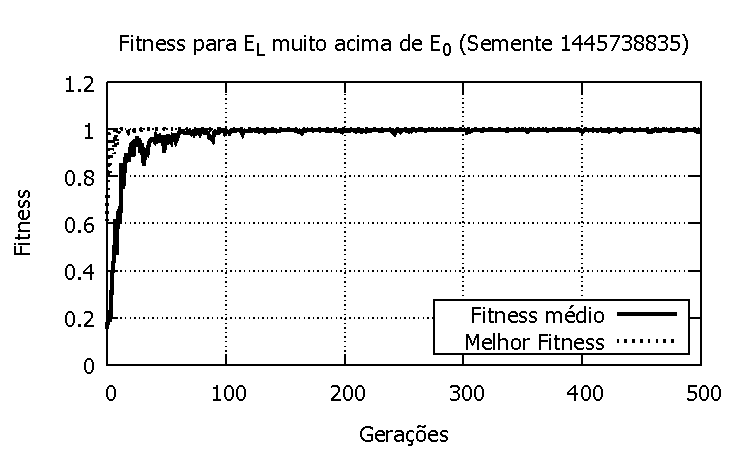
\includegraphics[width=.45\textwidth]{figs/resultados/variandoELSemente/T3_S-1445738835_fitness.pdf} &
    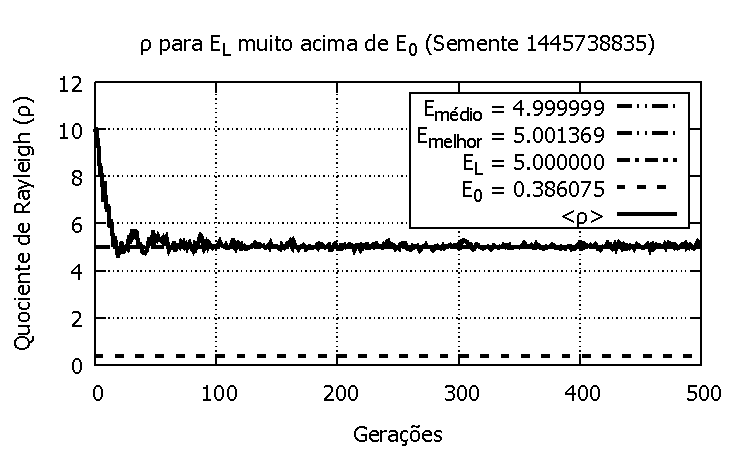
\includegraphics[width=.45\textwidth]{figs/resultados/variandoELSemente/T3_S-1445738835_rho.pdf}
  \end{tabular}
  \caption{Execução para a semente 1445738835. $E_L$ muito acima de $E_0$ no \textit{fitness} $f_i = e^{-\lambda(\rho_i - E_L)^2}$.}
	\label{fig:execucoesSemente_EL_umMuitoAcima}
	\end{figure}
	
	
	Semente 1445738835. Tipo 4. $E_L$ muito abaixo. Hipótese: não encontrará, muito distante. O \emph{fitness} ficou praticamente zero. Havia variabilidade no início, mas, como o \emph{fitness} foi zero pra todos, não havia como distinguir os melhores indivíduos. Entre as gerações 0 e 500 houve convergência genética precoce, estabilizando a média dos $\rho$ em aproximadamente 5.9 (verificar), que não é nenhum autovalor pra N = 10. 
	
	\begin{figure}[htbp]
	\centering
  \begin{tabular}{@{}cc@{}}	
		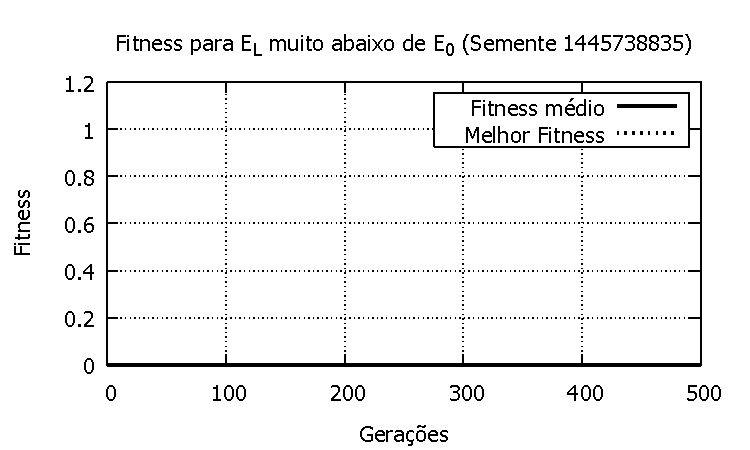
\includegraphics[width=.45\textwidth]{figs/resultados/variandoELSemente/T4_S-1445738835_fitness.pdf} &
    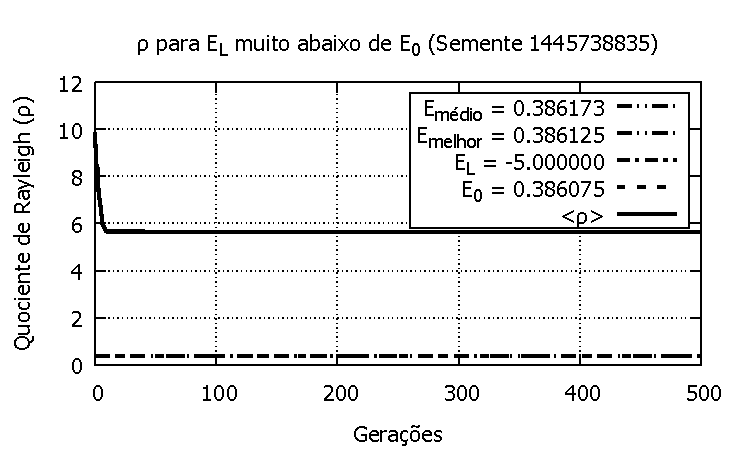
\includegraphics[width=.45\textwidth]{figs/resultados/variandoELSemente/T4_S-1445738835_rho.pdf}
  \end{tabular}
  \caption{Execução para a semente 1445738835. $E_L$ muito abaixo de $E_0$ no \textit{fitness} $f_i = e^{-\lambda(\rho_i - E_L)^2}$. Até geração 500.}
	\label{fig:execucoesSemente_EL_umMuitoAbaixo500}
	\end{figure}
	
	Entretanto, houve convergência para o autovalor mínimo. Um pouco antes da geração 32.000aconteceu um salto no \emph{fitness}, causado possivelmente por mutações (argentar). Apesar do \emph{fitness} médio ainda ser pequeno (<$f_i$>$< 0.025$), o \emph{crossover} com a nova informação genética criou variabilidade suficiente para chegar ao autovalor mínimo.
	
	\begin{figure}[htbp]
	\centering
  \begin{tabular}{@{}cc@{}}	
		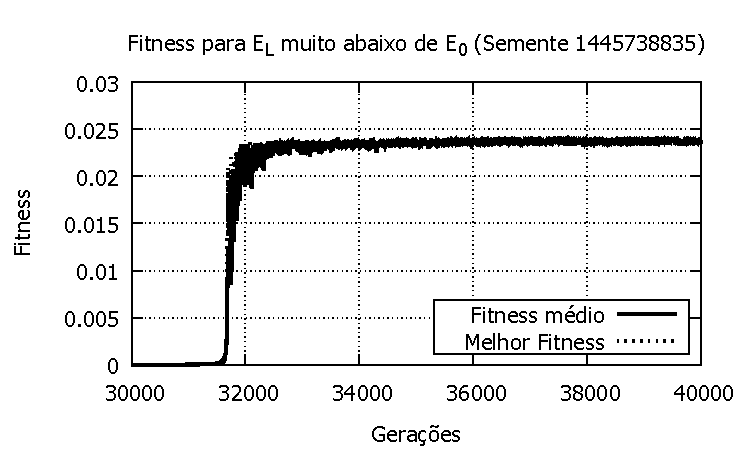
\includegraphics[width=.45\textwidth]{figs/resultados/variandoELSemente/T4_S-1445738835_fitness-extendido.pdf} &
    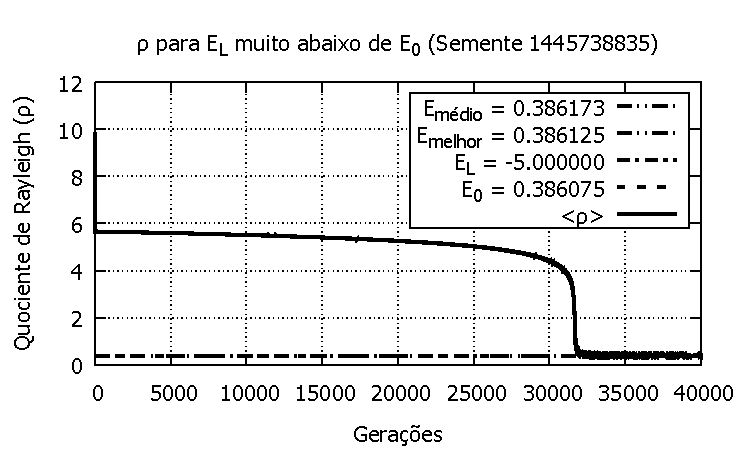
\includegraphics[width=.45\textwidth]{figs/resultados/variandoELSemente/T4_S-1445738835_rho_extendido.pdf}
  \end{tabular}
  \caption{Execução para a semente 1445738835. $E_L$ muito abaixo de $E_0$ no \textit{fitness} $f_i = e^{-\lambda(\rho_i - E_L)^2}$. Geração entre 30.000 e 40.000.}
	\label{fig:execucoesSemente_EL_umMuitoAbaixo40000}
	\end{figure}
	

	Na tabela \ref{VariandoELPraPrimeiraExecucao} há os valores desses testes. Como nas tabelas anteriores, os valores médios de $\rho$ e do \emph{fitness} (<$\rho$> e <\emph{fitness}>) foram calculados na geração final, ou seja, na população que atingiu algum dos critérios de parada. O <$\rho$> foi comparado com $E_0 = 0,386075$ para calcular o erro relativo (coluna Erro do <$\rho$> (\%)).
	
	

%\begin{landscape}
\begin{center}	
\begin{table}[htbp]
\caption{Variando $E_L$ para a execução da semente 1445738835. Os tipos de teste são: \textit{tipo 1}: $E_L$ um pouco acima de $E_0$; \textbf{tipo 2}: $E_L$ um pouco abaixo de $E_0$; \textbf{tipo 3}: $E_L$ muito acima de $E_0$; \textbf{tipo 4}: $E_L$ muito abaixo de $E_0$.}
\label{tab:VariandoELPraPrimeiraExecucao}
\scalefont{0.7}
\centering
% Table generated by Excel2LaTeX from sheet 'Plan2'
\begin{tabular}{cccccccc}
\hline \hline
\textbf{Teste} &  \textbf{$E_L$} & \textbf{Geração final} & \textbf{<$\rho$>} & \textbf{$\sigma$} & \textbf{Erro do <$\rho$> (\%)} & \textbf{|$\nabla \rho$|} & \textbf{<\emph{Fitness}>} \\
\hline \hline
         1 &   0,387000 &     42.577 &     0,3870 &     0,0004 &      0,2\% &    0,00009 &   1,000000 \\
\hline
         2 &   0,385000 &    400.000 &    0,38615 &    0,00003 &     0,02\% &   0,000006 &   1,000000 \\
\hline
         3 &   5,000000 &      9.622 &       5,00 &       0,02 &     1195\% &      0,003 &   0,999966 \\
\hline
         4 &  -5,000000 &    400.000 &    0,38617 &    0,00003 &     0,03\% &     0,0003 &   0,023843 \\
\hline \hline
\end{tabular}   
\end{table}
\end{center}	
%%\end{landscape}
	
\begin{landscape}
\begin{center}	
\begin{table}[htbp]
\caption{Cinco execuções para cada tipo de teste de variação de $E_L$ em torno de $E_0$ no fitness $f_i = e^{-\lambda(\rho_i - E_L)^2}$.}
\label{tab:VariandoELCincoExecucoes}
\centering
% Table generated by Excel2LaTeX from sheet 'Plan2'
\begin{tabular}{ccccccccc}
\hline \hline
\textbf{Teste} & \textbf{Execução} & \textbf{Semente} & \textbf{Geração final} & \textbf{<$\rho$>} & \textbf{$\sigma$} & \textbf{Erro do <$\rho$> (\%)} & \textbf{|$\nabla \rho$|} & \textbf{<\emph{Fitness}>} \\
\hline \hline
         1 &          1 & 1448150274 &     47.945 &     0,3870 &     0,0005 &  0,00005\% &    0,00008 &   1,000000 \\
\hline
         1 &          2 & 1448150289 &     24.128 &     0,3870 &     0,0004 & -0,00004\% &    0,00008 &   1,000000 \\
\hline
         1 &          3 & 1448150298 &     40.795 &     0,3870 &     0,0003 & 0,000007\% &    0,00008 &   1,000000 \\
\hline
         1 &          4 & 1448150315 &     17.047 &     0,3870 &     0,0005 &  -0,0001\% &     0,0001 &   1,000000 \\
\hline
         1 &          5 & 1448150321 &     16.284 &     0,3870 &     0,0003 &  0,00002\% &    0,00008 &   1,000000 \\
\hline \hline
         2 &          1 & 1448150327 &    400.000 &    0,38616 &    0,00003 &     0,02\% &   0,000009 &   1,000000 \\
\hline
         2 &          2 & 1448150472 &    400.000 &    0,38613 &    0,00002 &     0,01\% &   0,000005 &   1,000000 \\
\hline
         2 &          3 & 1448150600 &    400.000 &    0,38613 &    0,00002 &     0,02\% &   0,000005 &   1,000000 \\
\hline
         2 &          4 & 1448150704 &    400.000 &    0,38624 &    0,00008 &     0,04\% &    0,00002 &   1,000000 \\
\hline
         2 &          5 & 1448150809 &    400.000 &    0,38624 &    0,00007 &     0,04\% &    0,00001 &   1,000000 \\
\hline \hline
         3 &          1 & 1448150912 &      8.074 &       5,00 &       0,05 &  0,00002\% &      0,007 &   0,999750 \\
\hline
         3 &          2 & 1448150914 &     14.604 &       5,00 &       0,03 & -0,000005\% &      0,009 &   0,999889 \\
\hline
         3 &          3 & 1448150918 &     41.659 &       5,00 &       0,02 & -0,00002\% &      0,003 &   0,999954 \\
\hline
         3 &          4 & 1448150929 &      9.775 &       5,00 &       0,03 & 0,000009\% &      0,006 &   0,999886 \\
\hline
         3 &          5 & 1448150932 &     12.637 &       5,00 &       0,03 & -0,0000006\% &      0,005 &   0,999904 \\
\hline \hline
         4 &          1 & 1448150935 &    400.000 &     0,3864 &     0,0001 &     0,07\% &      0,001 &   0,023837 \\
\hline
         4 &          2 & 1448151040 &    400.000 & 7,98166818 & 0,00000001 &     1967\% &        6,0 &   0,000000 \\
\hline
         4 &          3 & 1448151146 &    400.000 & 10,564998429558 & 0,000000000002 &     2637\% &        8,6 &   0,000000 \\
\hline
         4 &          4 & 1448151251 &    400.000 &    0,38613 &    0,00002 &     0,02\% &     0,0003 &   0,023844 \\
\hline
         4 &          5 & 1448151357 &    400.000 &    0,38614 &    0,00003 &     0,02\% &     0,0003 &   0,023844 \\
\hline \hline
\end{tabular}  
\end{table}
\end{center}	
\end{landscape}
		
	\section{Por que o $\lambda$ deve ser escolhido cuidadosamente?}
	
	Execuções para N=10 com diferentes $\lambda$'s. Com os gráficos, explicar o que o artigo de 2004 quis dizer com \textit{fitness overflow/underflow}.
	
	Gráficos com rho entre 0 e 250 (exemplo pra N=10), mas com cortes em diferentes rhos.

	Explicar que uma boa escolha do $\lambda$ deve cobrir todos os autovalores. Citar as execuções anteriores (boas e ruins em função de cada $\lambda$).
	
	Gráfico com $\lambda$ fazendo o fitness cortar em um $\rho$ muito baixo. Discutir puxando as execuções anteriores.
	
	Outro gráfico, mas com $\lambda$ fazendo o fitness cortar em um $\rho$ muito alto. Discutir puxando as execuções anteriores.
	
	Gráfico com uma boa escolha de $\lambda$. Discutir puxando as execuções anteriores.
	
	Após estimativa, refinar a obtenção do $\lambda$. Alterar o $lambda$ (valores em torno da estimativa), executar o programa para verificar se o fitness médio da primeira população é baixo. (se a população inicial tem fitness muito grande, há convergência prematura).
	
	Tabela com alguns $lambdas$ encontrados dessa maneira (estimativa e refinamento).
	
	Infelizmente, para cada matriz, um $\lambda$ diferente.
	
	Ponte pra equação empírica do $\lambda$.
	
	\section{Equação empírica para o $\lambda$}
	
	Delineamento da equação como feito na reunião de 29/09.
	
	Isolar $\lambda$ a partir da $f=e^{-\lambda*(\rho - \rho_0)^2}$
	
	Fazer $f = 0.00001 \approx 0$.
	
	Substituir $(\rho - \rho_0)^2$ por $E_{central} - E_{mínimo}$. Justificar.
	
	Regressão linear para $E_{central} - E_{mínimo}$ com função apenas da ordem da matriz (N).
	
	Inserir a Equação obtida na regressão na equação de $\lambda$.
	
	Fator $0.65$: obtido empiricamente de modo que o $\lambda$ seja semelhante aos encontrados pelo processo de estimativa e refinamento.
	
	Exemplo de execução com $\lambda$ automático.
	
	Explicitar que essa equação é válida apenas para matrizes de Coope$-$Sabo. Apesar disso, foi importante para o estudo pois permitiu automação completa.
		
	\section{A mistura de $(\rho - \rho_0)^2$ com $\nabla\rho$ não leva a melhores resultados}
	
	Como em seção anterior verificamos que $f_i = e^{[-\lambda \nabla \rho]}$ é mais rápido do que $f_i = e^{[-\lambda (\nabla \rho)]}$, e que o $\nabla\rho$ está diretamente associado aos autovalores, pensei na seguinte hipótese: inserir $\nabla \rho$ ao fitness com $(\rho - \rho_0)^2$ traria resultados mais rápidos.
	
	Justificativas para a hipótese: 
	
	\begin{enumerate}
		\item Inserir $\nabla \rho$ no fitness puniria os $\rho$'s que, apesar de próximos de $\rho_0$, não fossem autovalor. Em outras palavras, o termo $\rho - \rho_0 \approx 0$, mas $\nabla \rho >> 0$ e, portanto, o fitness ficaria pequeno.
		
		\item Como o fitness, a princípio, estaria diferenciamento melhor os bons indivíduos, o algoritmo teria uma taxa de convergência maior.
		
	\end{enumerate}
	
		Executar $10$ para o primeiro fitness, e, utilizando as mesmas dez sementes, executar outros $10$ testes com ou outro fitness.
		
		Comparação dos resultados: gráficos do comportamento do fitness e tabela comparando a velocidade de convergência (em que geração o critério de parada foi atingido), tempo de execução e erro relativo ao menor autovalor ``exato'' (obtido no SciLab).

	\section{$f_i = e^{[-\lambda \nabla \rho]}$ é mais rápido do que $f_i = e^{[-\lambda (\nabla \rho)^2]}$}
	
	Como um dos critérios de parada utiliza $\nabla \rho$ (sem quadrado), testamos essa forma no fitness.
	
	Várias execuções.
	
	Gráfico comparando o comportamento (um termina mais rápido)
	
	Tabela com os detalhes explícitos do do ganho.
	
	Ponte pra falar sobre o outro fitness que encontra o mínimo.
	
	\section{Resultados preliminares na GPU}
	
		O GA aqui desenvolvido buscou a solução do problema ONEMAX, cujo objetivo é encontrar uma sequência de $N$ bits com a maior quantidade possível de “1” a partir de uma sequência aleatória de “1” e “0”. O ONEMAX é especialmente indicado para o início dos estudos em GA. Além de permitir simples implementação, possui representação cromossomial binária que, junto com o crossover de ponto único, forma a base da teoria original de Holland \cite{Linden2008}.

	O programa paralelizado foi uma tradução literal do seu equivalente serial para a sintaxe do CUDA C. Ou seja, não houve nenhuma mudança estrutural no código, seja nas variáveis e estruturas de dados, seja na ordem de execução das funções e procedimentos. Apenas o preenchimento aleatório da população inicial é executado na CPU, de forma que o núcleo do programa é executado inteiramente na GPU \cite{onemaxNaGPU}. 

	A população do GA era constituída por indivíduos formados por cromossomos com \textit{\texttt{numGenes}} elementos do tipo \texttt{char}. Cada elemento do vetor (gene) podia ter um valor  “1” ou “0”. Dentro do problema ONEMAX, os melhores indivíduos foram os que apresentaram maior número de genes iguais a “1”.
		
	\begin{figure}[htbp]
		\centering
			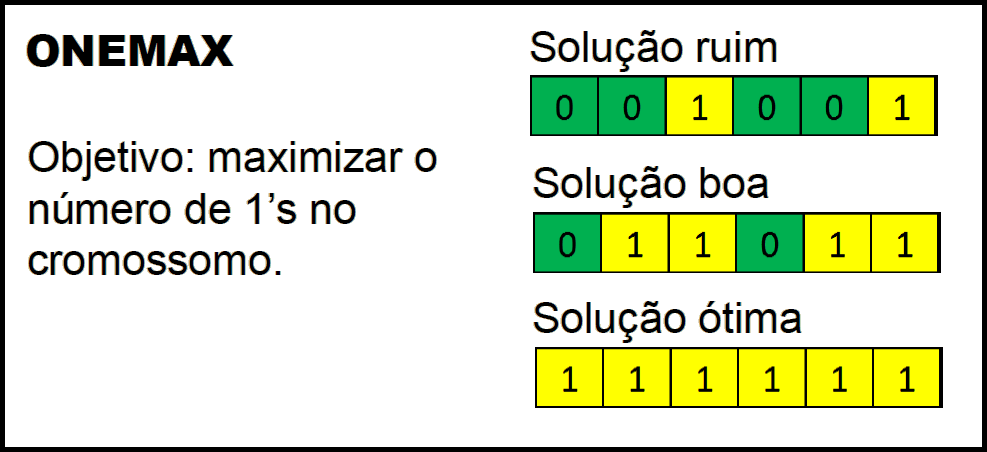
\includegraphics[width=0.50\textwidth]{figs/resultados/onemax/onemax_objetivo.png}
		\caption{ONEMAX, um problema clássico nos Algoritmos Genéticos.}
		\label{fig:onemax_objetivo}
	\end{figure}
		
	Implementei um \emph{kernel} (função que tem sua execução feita pela GPU) para cada um dos quatro passos do GA: cálculo da função avaliadora (\emph{fitness}), seleção, \emph{crossover} e mutação. Eles são chamados um após o outro até que um número máximo de gerações seja atingido. Isso é feito dentro do \emph{loop} principal (realizado na CPU), mas sem troca de informação entre CPU e GPU.
	
	No início do programa duas gerações são alocadas na memória global da GPU, as quais são usadas alternadamente como \emph{input} e \emph{output} dos kernels. Apenas as chamadas dos kernels acontecem na CPU, enquanto o restante (execução + dados) está na GPU. Todos os \emph{kernels} tinham como \emph{input} e \emph{output} uma estrutura do tipo Geração. Ou seja, as funções operaram sobre toda a população do GA, levando-nos a adotar como estratégia o paralelismo no nível dos indivíduos.
	
	\begin{figure}[htbp]
		\centering
			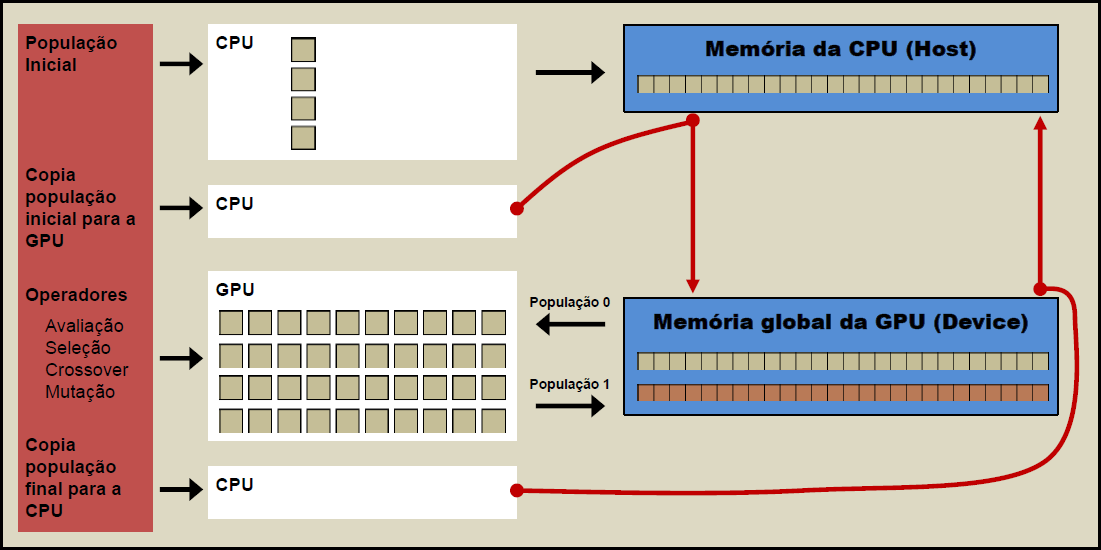
\includegraphics[width=1.00\textwidth]{figs/resultados/onemax/onemax_execucao.png}
		\caption{Execucao do ONEMAX paralelo. Apenas as chamadas dos kernels acontecem na CPU, enquanto o restante (execução + dados) está na GPU.}
		\label{fig:onemax_execucao}
	\end{figure}
		
	No cálculo do \emph{fitness}, o \emph{input} foi uma população com \textit{\texttt{numIndividuos}} e o \emph{output} uma população com os mesmos \textit{\texttt{numIndividuos}} e suas respectivas notas. O cálculo do \emph{fitness} de cada indivíduo foi realizado por meio da soma dos valores de seus genes. Por exemplo, para um indivíduo formado por um cromossomo de 6 genes (\textit{\texttt{numGenes}} = 6) com a configuração “010101”, o valor do fitness é 3 e a solução ótima para esse caso seria “111111” (figura \ref{fig:onemax_objetivo}). No código serial a programação é simples e envolve apenas um laço for que percorre o cromossomo e soma os bytes. Porém, note que toda informação necessária para esse cálculo está contida no próprio cromossomo, ou seja, a obtenção do \emph{fitness} de um dado indivíduo não depende do restante da população. Assim, a paralelização do cálculo do \emph{fitness} deu-se por meio da associação de uma \emph{thread} para cada indivíduo.
	
	Para o operador de seleção, optei pela seleção via torneio com o tamanho do torneio fixo e igual a dois. Novamente, o \emph{input} e o \emph{output} são populações. Na entrada há \textit{\texttt{numIndividuos}} e suas notas. Os mais aptos (maiores \emph{fitness}) têm maiores chances de serem selecionados, e compõem os \textit{\texttt{numIndividuos}} da população na saída. Assim como no cálculo do \emph{fitness}, o paralelismo acontece no nível dos indivíduos. Para cada indivíduo na população de saída há uma \emph{thread}, que seleciona aleatoriamente dois cromossomos na população da entrada (memória global) e fica com o de maior \emph{fitness}.

O \emph{input} do \emph{crossover} é a população resultante da seleção. Utilizei o \emph{crossover} de dois pontos, independentemente da quantidade de genes do cromossomo, com probabilidade $p_C = 90\%$. Na implementação serial, apenas um indivíduo é gerado ao término do \emph{crossover}. Isso garantiu que, na versão paralela, a chamada da função de \emph{crossover} fosse configurada com exatamente o mesmo número de \emph{threads} dos operadores anteriores (avaliação e seleção): uma \emph{thread} para cada indivíduo na população de saída, que recebe um cromossomo resultante do \emph{crossover}.

Após o \emph{crossover} todos os indivíduos passam por uma mutação simples, onde cada gene do cromossomo tem baixa probabilidade (0,01\%) de ser invertido (0 $\rightarrow$ 1 ou 1 $\rightarrow$ 0). Logo, semelhante ao cálculo do \emph{fitness}, a mutação em um dado indivíduo é independente do restante da população. Mais uma vez, uma \emph{thread} foi associada a cada \textit{\texttt{iIndividuo}} cromossomo na saída, que recebe os genes modificados do \textit{\texttt{iIndividuo}} na entrada. 

	Os experimentos foram executados em um laptop equipado com uma CPU Intel Core 2 Duo T6600 - 2,2 GHz. A placa de vídeo utilizada foi uma GeForce G 130M, com quatro multiprocessadores a 1,5 GHz e memória global total de 466 MB. A versão da API CUDA foi a 4.0, programada com o Microsoft Visual C++ Express 2008.
	
	A placa G 130M possui capacidade de computação 1.1 (que indica a versão do hardware de computação presente na GPU). Comparada com a primeira versão (arquitetura original da G80), ela adiciona suporte à operações na memória global que permitem que múltiplas \emph{threads} executem, sem conflito, operações ler-modificar-escrever na memória. Como o suporte às operações de ponto flutuante com precisão dupla só foi disponibilizado na versão 1.3, tanto o programa serial quanto o paralelo utilizaram precisão simples.
	
	As medidas de desempenho foram feitas com o objetivo de observar a influência de dois parâmetros do GA: i) número de indivíduos na população e ii) tamanho do cromossomo. O ganho na velocidade foi calculado como a razão entre o tempo de execução do programa serial e o tempo de execução do programa paralelo.

Verifiquei que o ganho de desempenho da versão paralela do GA cresce com o aumento do número de indivíduos (figura \ref{fig:ganhoNumInd}). O programa serial é mais rápido (ganho < 1) para populações pequenas (< 50). Porém, a partir de uma população de 50 indivíduos, o programa paralelo apresenta desempenho superior. Com 600 indivíduos, a versão paralela é oito vezes mais rápida para um cromossomo de tamanho 10, e dez vezes para um cromossomo de tamanho 300. 

\begin{figure}[htbp]
	\centering
		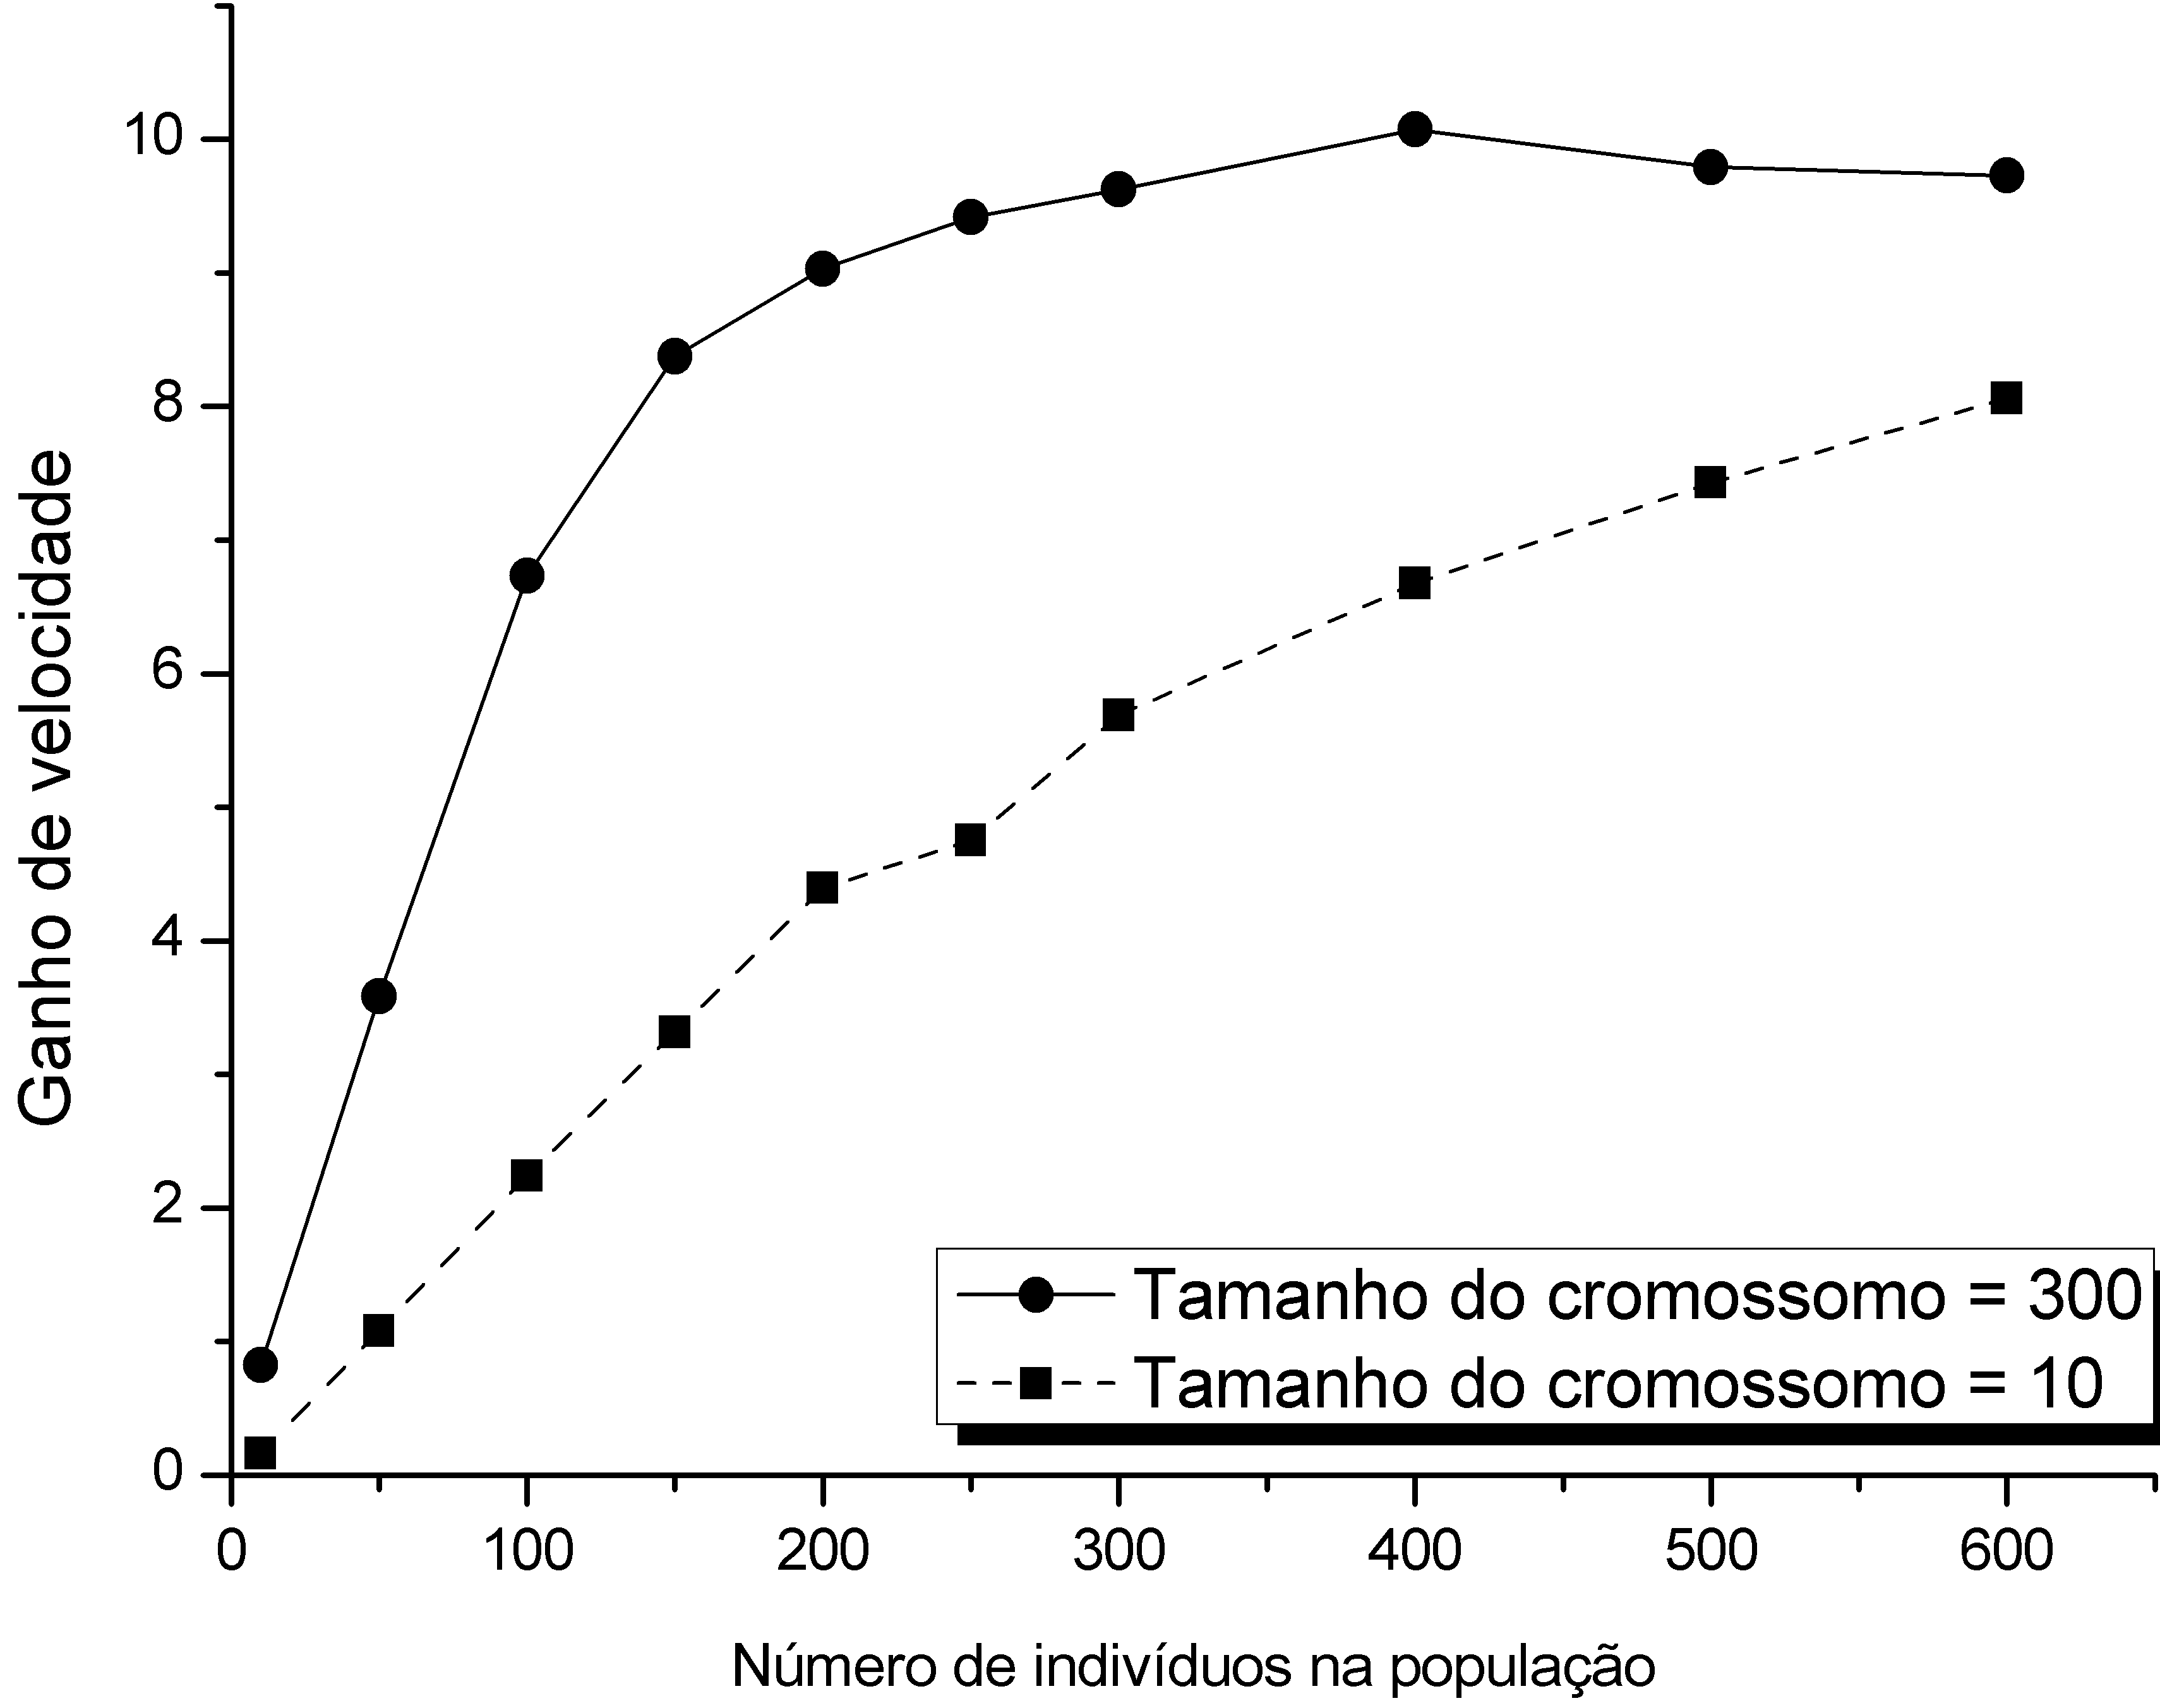
\includegraphics[width=0.70\textwidth]{figs/resultados/onemax/ganhoNumInd.png}
	\caption{ONEMAX paralelo. Ganho de velocidade em função do número de indivíduos da população.}
	\label{fig:ganhoNumInd}
\end{figure}

	Ao analisarmos a influência do tamanho do cromossomo verificamos um comportamento aproximadamente constante do ganho (figura \ref{fig:ganhoTamCromo}). Isso era esperado, pois a paralelização ocorreu no nível dos indivíduos e não no nível dos cromossomos. Com 600 indivíduos o ganho fica em torno de 9x para qualquer tamanho de cromossomo. O comportamento se repete com uma população de 10 indivíduos, mas, nesse caso, o programa serial sempre é mais rápido, mesmo para cromossomos muito pequenos (ganho sempre < 1). 
		
	\begin{figure}[htbp]
		\centering
			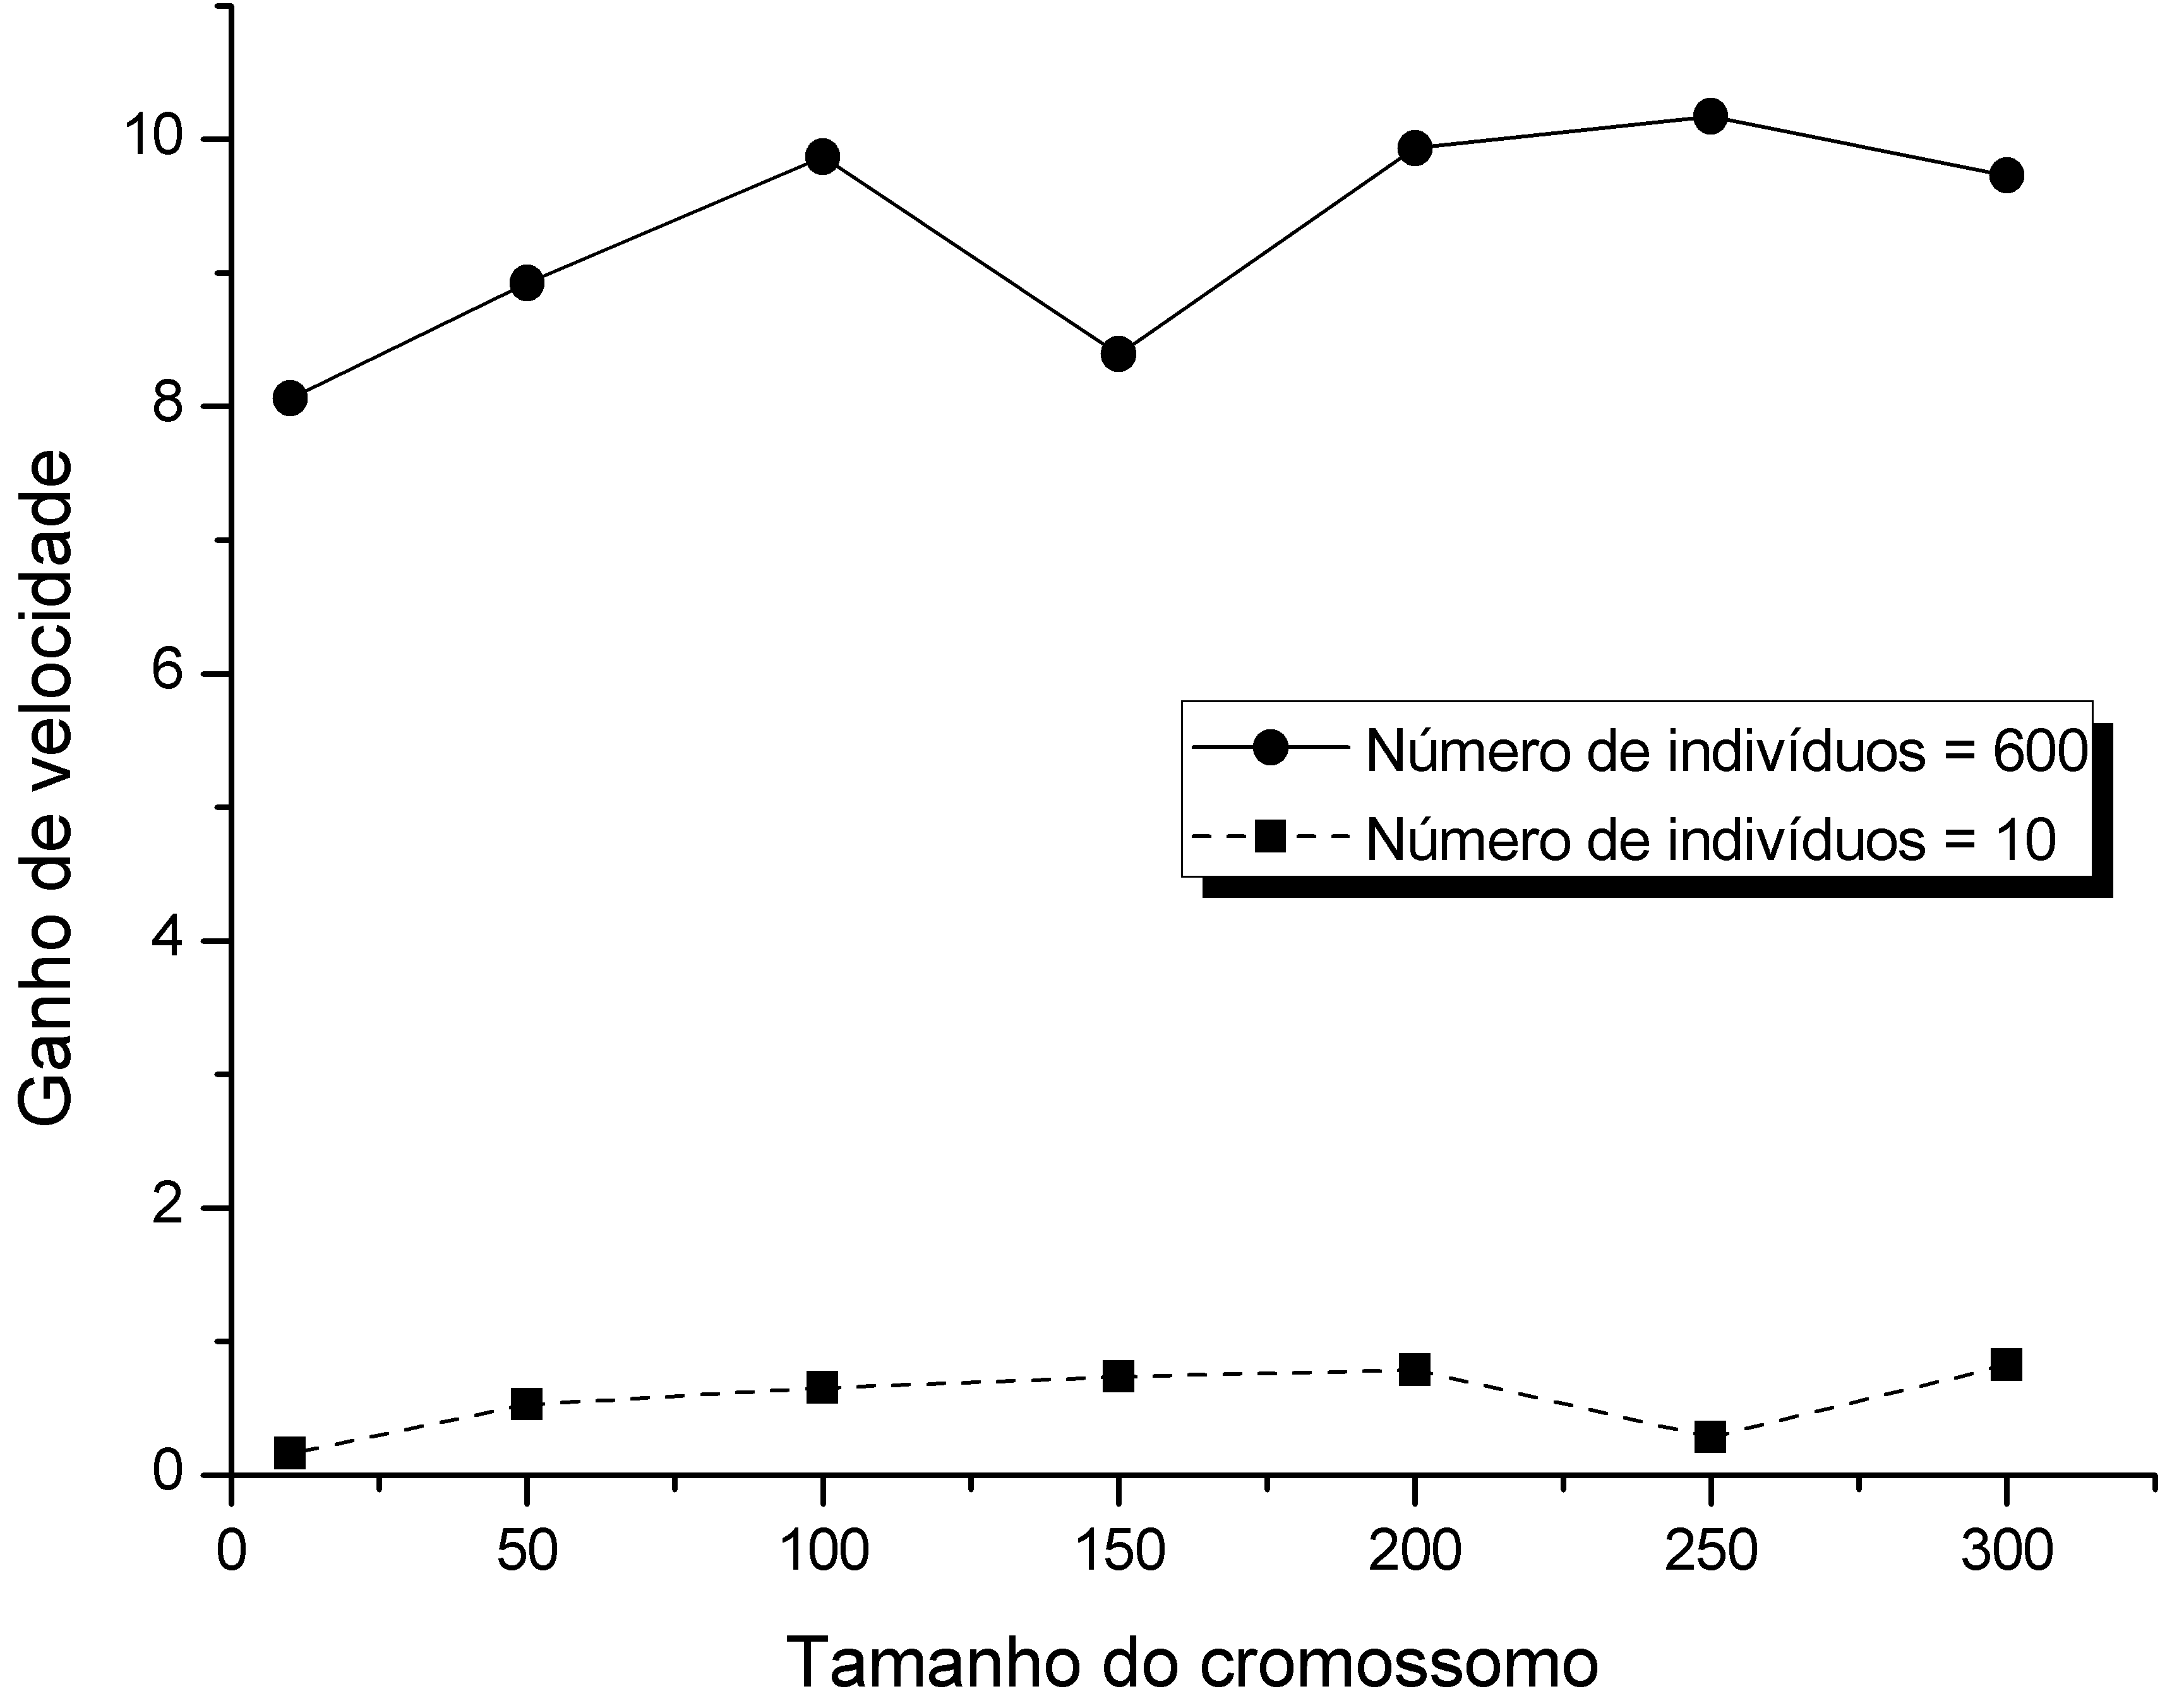
\includegraphics[width=0.70\textwidth]{figs/resultados/onemax/ganhoTamCromo.png}
		\caption{ONEMAX paralelo. Ganho de velocidade em função do tamanho do cromossomo.}
		\label{fig:ganhoTamCromo}
	\end{figure}

% --- Finaliza a parte no bookmark do PDF, para que se inicie o bookmark na raiz ---
\bookmarksetup{startatroot}%

% ---- ELEMENTOS PóS-TEXTUAIS ----
\postextual

% ---- Referências bibliográficas ----
\bibliography{tese}

% ---- Apêndices ----
\begin{apendicesenv}
% Imprime uma página indicando o início dos apêndices
\partapendices

\chapter{Autovalores do século $\mathsf{XVIII}$ ao $\mathsf{XXI}$}\label{apdx:historia}
	
	A primeira aparição do que hoje é chamado de autovalor aconteceu em 1743 \cite{Hawkins75}. Estudando o problema de várias massas ligadas umas às outras por molas, D'Alembert chegou a um sistema de equações diferenciais. Ao fazer algumas transformações de variáveis ele foi capaz de reduzir o estudo a apenas uma equação:

\begin{equation}\label{eq:EDO1}
	\frac{d^2u}{dt^2} + \lambda u = 0,
\end{equation}
sendo $u$ uma soma envolvendo o produto das velocidades e posições de cada massa, e $\lambda$ um escalar. D'Alembert aplicou o novo método a sistemas com duas e três massas ($n = 2$ ou $n = 3$) e, com argumentos relacionados à Física do problema, afirmou que $\lambda$ só poderia ser real. A partir de então, diversos matemáticos se dedicaram ao assunto.

	Na metade do século $\mathsf{XVIII}$, D'Alembert, aproveitando trabalho anterior de Euler, demonstrou que as soluções gerais da equação \ref{eq:EDO1} são da forma $g\mathsf{e}^{-\lambda t}$, $g$ sendo um escalar, e que $\lambda$ está associado com a estabilidade do sistema massa--mola. Lagrange estende a solução para $n$ massas e escreve a equação polinomial característica, mas naquele tempo nada se sabia sobre a natureza de suas raízes. Em 1775 ele aplica seu método para a rotação de corpos rígidos desenvolvida por Euler dez anos antes, e é a primeira vez que autovalores são utilizados fora do contexto massa--mola. Em seguida, em 1778, o mesmo Lagrange mostra que a mecânica celestial pode ser escrita como um sistema de equações diferenciais, e conclui que $\lambda$ está ligado à natureza das órbitas e à estabilidade do Sistema Solar.
	
	Entra em cena Laplace, descobrindo em 1784 que $\lambda$ depende \emph{apenas} dos coeficientes $A_{ij}$ envolvidos nos sistemas de equações diferenciais. Quatro anos depois mostra que um sistema discreto de massas próximo do equilíbrio pode ser escrito como 
	
	\begin{equation}
		\mathsf{B}\mathsf{X} = \lambda \mathsf{A}\mathsf{X},
	\end{equation}
	com as matrizes $\mathsf{B}$ e $\mathsf{A}$ ligadas, respectivamente, à Energia Potencial e Energia Cinética do sistema. Embasado na Convervação da Energia, argumenta que os autovalores $\lambda$ são reais, positivos e distintos. Finalmente, em 1789, Laplace percebe as simetrias envolvidas para construir o primeiro teorema, completo e com demonstração, da natureza dos autovalores.
	
	A partir do século $\mathsf{XIX}$ o problema dos autovalores e autovetores começa a tomar a forma que conhecemos hoje. Cauchy desenvolve em 1815 a Teoria dos Determinantes e em 1829 prova, com argumentos puramente matemáticos, que os autovalores de uma matriz simétrica são reais. Matrizes simétricas são quadradas, com elementos $a_{ij}$ reais, e $a_{ij} = a_{ji}$ para $i \neq j$. Nesse mesmo ano Sturn usa autovalores na Condução de Calor, levando as aplicações para além da Mecânica Clássica. Em 1839 Cauchy cunha o termo ``Equação Característica''. Em torno de 1855 os resultados obtidos por Cauchy tornam-se ``matemática básica'' entre os matemáticos da época.
	
	No artigo \cite{autovaloresSecXX} há uma revisão sobre o desenvolvimento do cálculo de autovalores no século $\mathsf{XX}$\footnote{É importante salientar que o problema de autovalores e autovetores foi fundamental em uma das grandes revoluções científicas e culturais da nossa era, a Mecânica Quântica.}. Impulsionado pelo advento do computador eletrônico na década de 1950, o alvo desse desenvolvimento foi a criação de métodos numéricos com convergência rápida e resultados precisos. Esponho aqui os dois tipos principais, os de potência e os que reduzem a matriz principal a uma forma mais eficiente.
	
	Os Métodos de Potência (\emph{Power Methods}) são mais simples. A ideia é multiplicar a matriz $\mathsf{A}$ repetidas vezes por um vetor inicial $\mathsf{x}$ bem escolhido, de modo que um de seus componentes, o que está na direção do autovetor associado ao maior autovalor em valor absoluto, é aumentado em relação aos outros componentes. Assim, obtém-se o maior autovalor. Uma variação mais efetiva é o Método da Potência Inverso (\emph{Inverse Power Method}), que trabalha com a matriz $(\mathsf{A} - \mu \mathsf{I})^{-1}$, onde $\mu$ é um valor de deslocamento em torno de $\mathsf{A}$ a cada iteração. Tais algoritmos não são mais competitivos, mas continuam sendo estudados pois formam a base de métodos modernos.
	
	Um deles é o Método da Iteração do Quociente de Rayleigh (\emph{Rayleigh Quotient Iteration}). Inspirado num algoritmo utilizado por Lord Rayleigh em 1870, usa um quociente de Rayleigh (equação \ref{eq:rho} do capítulo \ref{cap:algebra}) para o deslocamento $\mu$. O atual é muito rápido, e possui convergência cúbica [$O(n^3)$].
		
	Com relação aos métodos de redução, todos partem da ideia central que matrizes podem ser reduzidas a uma forma mais eficiente para as computações subsequentes, utilizando um número finito de passos em transformações ortogonais. Por exemplo, foi possível aproveitar a seguinte propriedade das matrizes simétricas: para qualquer matriz simétrica $\mathsf{A}$ sempre existe uma matriz $\mathsf{Q}$ de modo a fazer uma transformação do tipo $\mathsf{Q}^{\dag} \mathsf{A} \mathsf{Q} = \mathsf{D}$, em que $\mathsf{Q}^{\dag}$ é a transposta de $\mathsf{Q}$, $\mathsf{D}$ é diagonal e seus elementos são os autovalores de $\mathsf{A}$. O Método de Jacobi, desenvolvido em 1846, faz isso por meio de uma série de rotações. Originalmente não garantia convergência, problema que foi corrigido apenas em 1949.
	
	Em 1931 Kyrlov sugeriu um método baseado no fato de que toda matriz satisfaz sua equação (ou polinômio) característica(o). Ele usou os vetores $\mathsf{x}$, $\mathsf{A}\mathsf{x}$, $\mathsf{A}^2\mathsf{x}$ (...) gerados pelo método da potência para determinar os coeficientes dessa equação. A técnica não foi bem aceita porque era instável, pois pequenas modificações em $\mathsf{A}$ levam a grandes mudanças nos coeficientes do polinômio. Entretanto, ele teve sua importância pois inspirou os famosos métodos de Householder e Lanczos. O último, por exemplo, a partir de 1980 era o preferido para grandes matrizes simétricas e esparsas (com muitos zeros).
	
	 De acordo com \cite{autovaloresSecXX}, o Método QR era um dos mais populares e mais poderosos do ano 2000. Ele é capaz de calcular \emph{todos} os autovalores e autovetores de uma matriz simétrica e densa (não esparsa), sempre  com convergência cúbica [O($n^3$)].
	
	Porém, por volta de 1970 o rumo da pesquisa na área mudou. Naquela época o problema padrão para o cálculo numérico de autovalores (equação \ref{eq:detIntro}) foi visto como essencialmente resolvido para matrizes não muito grandes ($n \leq 25$). Então, além de tratar problemas generalizados e, consequentemente, mais complexos, o interesse voltou-se para matrizes maiores.
	
	Em 1981 Cuppen apresenta o primeiro algoritmo paralelo para matrizes tridiagonais de tamanho moderado, com $n > 25$ e menor do que alguns milhares. Da classe de algoritmos do tipo ``Divida e Conquiste'', a ideia foi dividir a matriz original em dois blocos com metade do tamanho original, além de gerar uma matriz que ele chamou de Matriz de Atualização. Cuppen mostrou como o problema de autovalores para cada um dos blocos poderia ser combinado para resolver o problema principal, e reconheceu que seu algoritmo era assintoticamente muito mais rápido que o QR. Novamente, problemas de instabilidade, principalmente relacionados aos autovetores de autovalores próximos, fizeram com que o método não fosse considerado competitivo para matrizes pequenas. Entretanto, ele continuou a ser desenvolvido pois apresentava propriedades paralelas interessantes. Após uma correção publicada em 1995 o método foi aceito pela comunidade.
	
	O século $\mathsf{XX}$ chega ao seu fim com \emph{software} consolidado, seja em forma de bibliotecas para uso de programadores, seja em ambientes numéricos comerciais e de código aberto. A biblioteca LINPACK cobriu soluções numéricas para sistemas lineares, enquanto a EISPACK se concentrou nos problemas de autovalores. A EISPACK foi substituída em 1995 pela LAPACK, que possui uma versão paralela, ScaLAPACK, cuja meta é fornecer \emph{software} para arquiteturas paralelas modernas. O ambiente MATLAB, comercial, está no estado da arte da computação para álgebra linear numérica, e tornou-se padrão na década de 1990. Boas alternativas não comerciais estão disponíveis, como o Octave e o SciLab.
		
	Autovalores continuam importantes no século $\mathsf{XXI}$. A busca pela palavra \emph{eigenvalue} em periódicos como \emph{Nature} e \emph{Science} leva a vários artigos em inúmeras áreas diferentes. Restringindo a pesquisa apenas ao ano de 2015, encontramos autovalores na descoberta de novos fármacos \cite{avMedicamento2015}, cultivo de cana de açúcar na China \cite{avCana2015}, física teórica \cite{avFisTeo2015} e ciência de materiais \cite{avCienciaMateriais2015}. No jornal PLOS ONE é possível navegar por artigos associados especificamente à palavra--chave \emph{eigenvalue}\footnote{\href{http://www.plosone.org/browse/eigenvalues}{http://www.plosone.org/browse/eigenvalues}}.
	
	Mas o destaque não está limitado apenas à ciência. O algoritmo \emph{PageRank}, base do mecanisno de busca do Google, tem em seu núcleo uma formulação do problema de autovalores e autovetores \cite{BrinPage98}. Em uma versão simplificada, define-se uma matriz quadrada $\mathsf{A}$ de modo que suas linhas e colunas representam páginas da \emph{Web}. Os elementos $\mathsf{A}_{u,v}$ são definidos de tal maneira que, se não houver um \emph{hyperlink} entre $u$ e $v$, $\mathsf{A}_{u,v} = 0$, caso contrário, $\mathsf{A}_{u,v}$ é inversamente proporcional ao número total de \emph{hyperlinks} que $u$ possui apontando para quaisquer outras páginas (uma característica, então, que depende apenas de $u$). A relevância das páginas (\emph{rank}) é definida como
	
	\begin{equation}
		\mathsf{\textbf{R}} = c\mathsf{A}\mathsf{\textbf{R}},
	\end{equation}
	onde $\mathsf{\textbf{R}}$ é o autovetor de $\mathsf{A}$ com autovalor associado $c$. O objetivo é encontrar o autovetor dominante, ou seja, aquele associado ao autovalor de maior valor absoluto. Ele terá as informações da ordem de relevância das páginas associadas à busca, da mais relevante para a menos. Ou seja, a ordem das páginas exibidas em uma busca no Google é a expressão direta de $\mathsf{\textbf{R}}$ na equação acima.
	
	Outra aplicação fundamental dos autovalores na atualidade está presente na Teoria Espectral dos Grafos, que ``\textit{busca analisar propriedades estruturais
de grafos através de matrizes e seus espectros, ou seja,
dos autovalores das matrizes associadas a eles}'' \cite{TEG2014}. Um grafo (ou rede) é um conjunto de itens, chamados de vértices ou nós, com conexões entre eles, chamadas de arestas. Na figura \ref{fig:grafo} há um exemplo. Há várias matrizes associadas a um grafo, e tem-se descoberto que seus autovalores trazem informações importantes sobre a estrutura da rede.
	
	\begin{figure}[htbp]
		\centering
			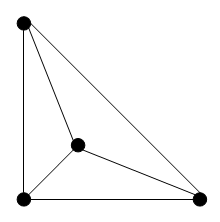
\includegraphics[width=0.33\textwidth]{figs/intro/grafo.PNG}
		\caption{Exemplo de um grafo. Fonte: Wikipedia.}
		\label{fig:grafo}
	\end{figure}
	
	Vários sistemas tomam a forma de redes, como a \emph{Web} e as Redes Sociais digitais \cite{Newman2003}. No caso do Facebook e Twitter, por exemplo, as redes são enormes, atingindo facilmente centenas de milhões de nós (usuários), levando a matrizes de dimensão equivalente a essa ordem de grandeza \cite{twitter2010}. Nesses casos, extrair informações estruturais por meio dos seus autovalores é uma tarefa desafiadora.
	
	Então, acredito que a pesquisa teória e computacional, assim como das aplicações dos autovalores, continuarão ativas por um bom tempo.
%\chapter{Lista de autovalores}

\begin{table}[htb]
	\caption{Lista de autovalores para matrizes de Coope$-$Sabo de ordem 10, 20, 30 e 40.}
	\label{tab:autovalores10a40}
% Table generated by Excel2LaTeX from sheet 'Todos'
\begin{center}
\begin{tabular}{r|r|r|r|r}
	\hline \hline
	\textbf{\#} &   \textbf{10} &   \textbf{20} &   \textbf{30} &   \textbf{40} \\
	\hline \hline
					 0 &   0,386075 &   0,341237 &   0,319737 &   0,306086 \\
	\hline
					 1 &   2,461056 &   2,397247 &    2,36844 &   2,350583 \\
	\hline
					 2 &   4,518931 &   4,436173 &   4,401134 &   4,379909 \\
	\hline
					 3 &   6,572897 &   6,468521 &   6,427419 &     6,4031 \\
	\hline
					 4 &   8,628524 &   8,497626 &   8,450274 &    8,42294 \\
	\hline
					 5 &   10,69057 &   10,52507 &   10,47105 &   10,44068 \\
	\hline
					 6 &   12,76574 &   12,55178 &    12,4905 &     12,457 \\
	\hline
					 7 &   14,86753 &   14,57845 &   14,50908 &   14,47232 \\
	\hline
					 8 &   17,03654 &   16,60562 &   16,52713 &   16,48692 \\
	\hline
					9 &   22,07215 &   18,63385 &   18,54488 &     18,501 \\
	\hline
					10 &            &    20,6637 &   20,56255 &    20,5147 \\
	\hline
					11 &            &   22,69588 &    22,5803 &   22,52816 \\
	\hline
					12 &            &   24,73127 &   24,59828 &   24,54146 \\
	\hline
					13 &            &   26,77114 &   26,61667 &   26,55469 \\
	\hline
					14 &            &   28,81733 &    28,6356 &   28,56792 \\
	\hline
					15 &            &   30,87288 &   30,65527 &   30,58122 \\
	\hline
					16 &            &   32,94325 &   32,67586 &   32,59466 \\
	\hline
					17 &            &   35,04014 &    34,6976 &   34,60831 \\
	\hline
					18 &            &   37,19805 &   36,72077 &   36,62223 \\
	\hline
					19 &            &    45,2308 &   38,74571 &   38,63648 \\
	\hline
					20 &            &            &   40,77285 &   40,65114 \\
	\hline
					21 &            &            &   42,80277 &    42,6663 \\
	\hline
					22 &            &            &   44,83625 &   44,68204 \\
	\hline
					23 &            &            &   46,87444 &   46,69846 \\
	\hline
					24 &            &            &   48,91902 &   48,71568 \\
	\hline
					25 &            &            &   50,97274 &   50,73385 \\
	\hline
					26 &            &            &   53,04052 &   52,75311 \\
	\hline
					27 &            &            &   55,13271 &   54,77369 \\
	\hline
					28 &            &            &   57,27946 &   56,79581 \\
	\hline
					29 &            &            &   68,37101 &   58,81981 \\
	\hline
					30 &            &            &            &   60,84608 \\
	\hline
					31 &            &            &            &   62,87517 \\
	\hline
					32 &            &            &            &   64,90781 \\
	\hline
					33 &            &            &            &   66,94504 \\
	\hline
					34 &            &            &            &   68,98845 \\
	\hline
					35 &            &            &            &   71,04053 \\
	\hline
					36 &            &            &            &   73,10578 \\
	\hline
					37 &            &            &            &   75,19353 \\
	\hline
					38 &            &            &            &   77,33102 \\
	\hline
					39 &            &            &            &   91,50634 \\
	\hline \hline
	\end{tabular}
	\end{center}  
\end{table}
%\chapter{Execuções para o \emph{fitness} $f_i = e^{-\lambda||\nabla\rho||^2}$}

\begin{figure}[htbp]
\centering
  \begin{tabular}{@{}cc@{}}
    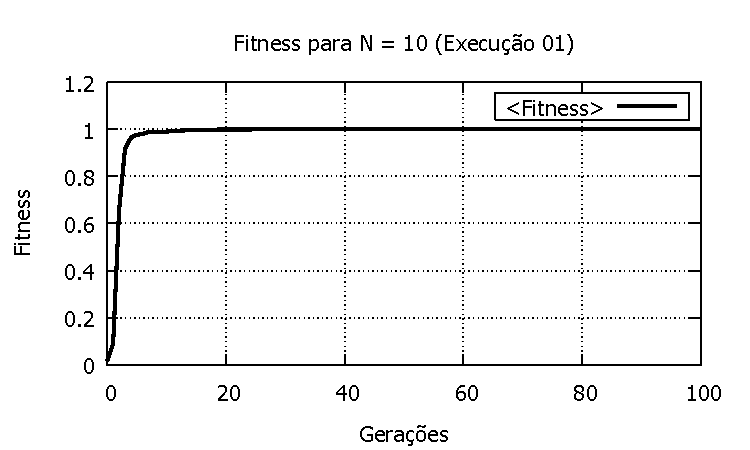
\includegraphics[width=.45\textwidth]{figs/resultados/fitnessGrad/N10_01_fitness.pdf} &
    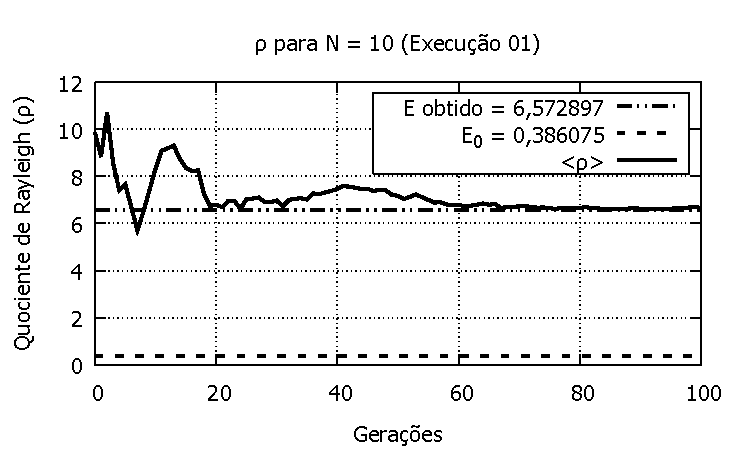
\includegraphics[width=.45\textwidth]{figs/resultados/fitnessGrad/N10_01_rho.pdf}   \\
		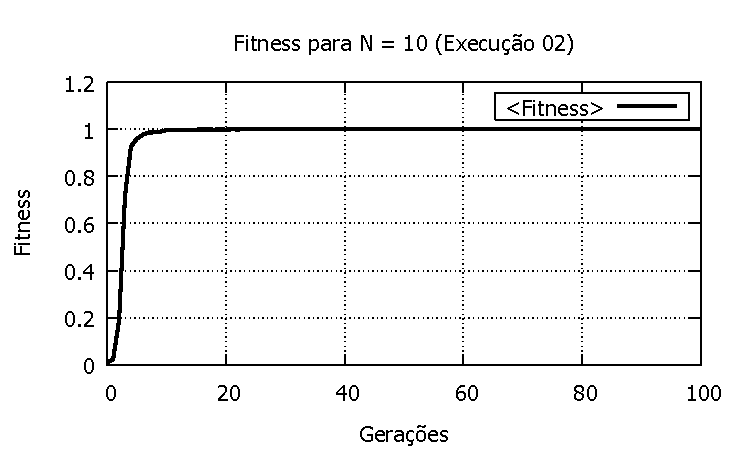
\includegraphics[width=.45\textwidth]{figs/resultados/fitnessGrad/N10_02_fitness.pdf} &
    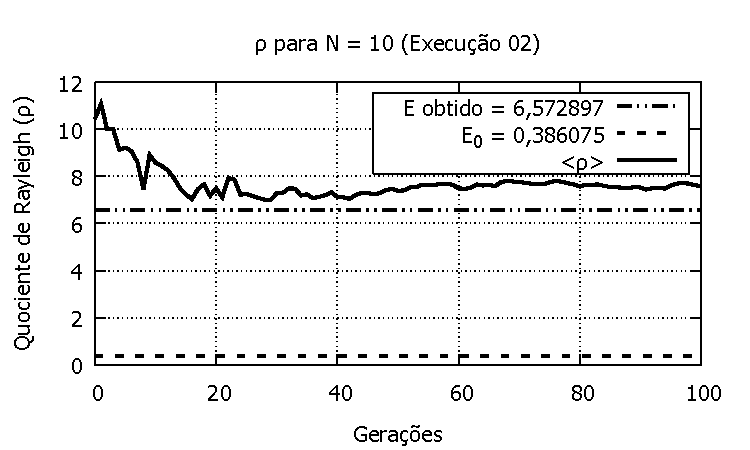
\includegraphics[width=.45\textwidth]{figs/resultados/fitnessGrad/N10_02_rho.pdf}   \\
		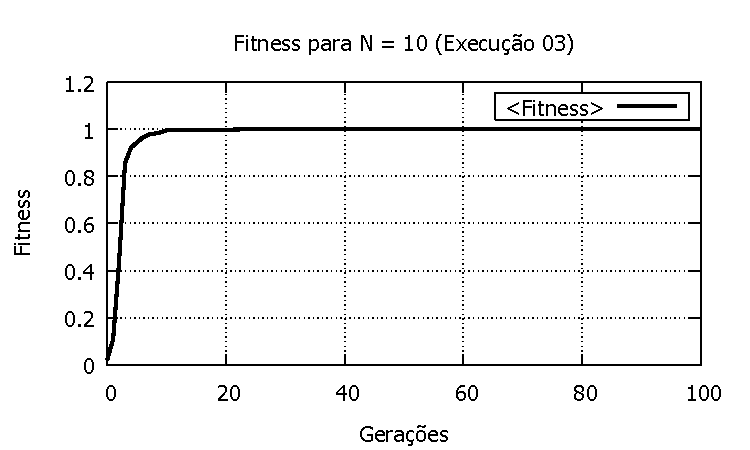
\includegraphics[width=.45\textwidth]{figs/resultados/fitnessGrad/N10_03_fitness.pdf} &
    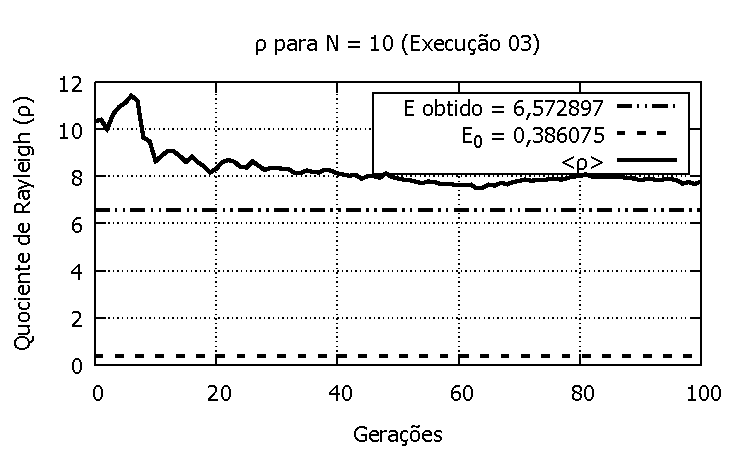
\includegraphics[width=.45\textwidth]{figs/resultados/fitnessGrad/N10_03_rho.pdf}   \\
		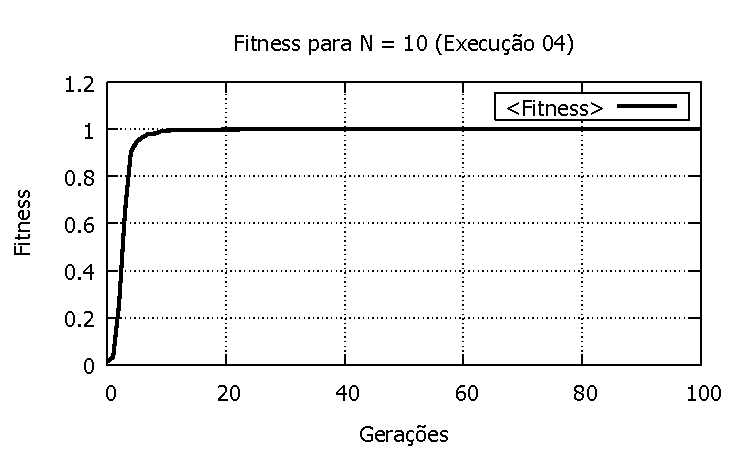
\includegraphics[width=.45\textwidth]{figs/resultados/fitnessGrad/N10_04_fitness.pdf} &
    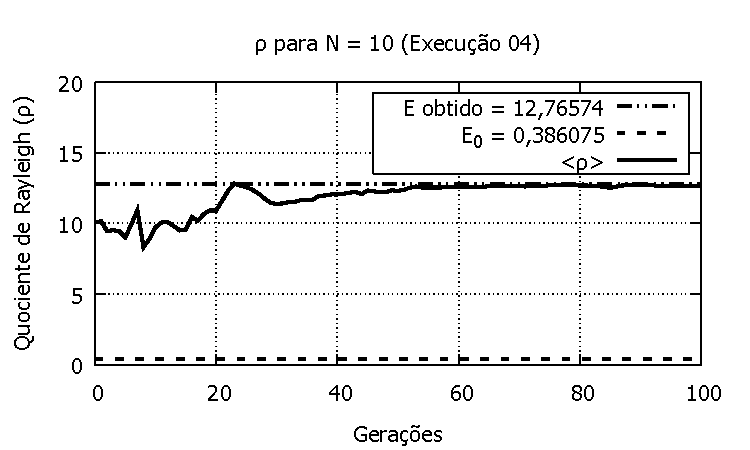
\includegraphics[width=.45\textwidth]{figs/resultados/fitnessGrad/N10_04_rho.pdf}   \\
		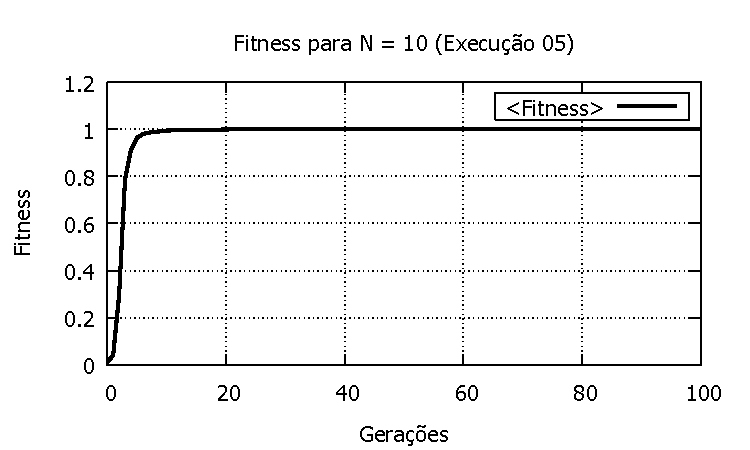
\includegraphics[width=.45\textwidth]{figs/resultados/fitnessGrad/N10_05_fitness.pdf} &
    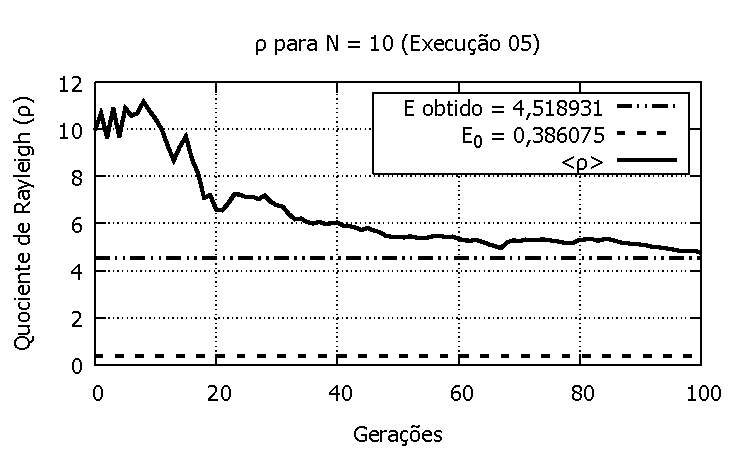
\includegraphics[width=.45\textwidth]{figs/resultados/fitnessGrad/N10_05_rho.pdf}
    %\multicolumn{2}{c}{\includegraphics[width=.23\textwidth]{example-image-a}}
  \end{tabular}
  \caption{Execuções N = 10.}
	\label{fig:execucoes_N10}
\end{figure}

\begin{figure}[htbp]
\centering
  \begin{tabular}{@{}cc@{}}
    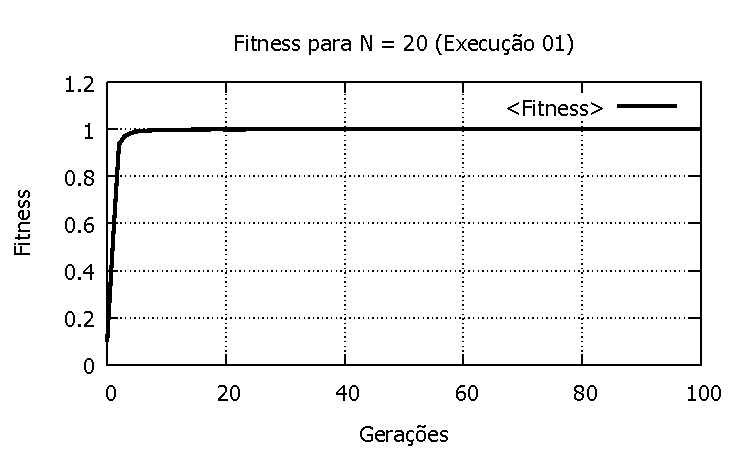
\includegraphics[width=.45\textwidth]{figs/resultados/fitnessGrad/N20_01_fitness.pdf} &
    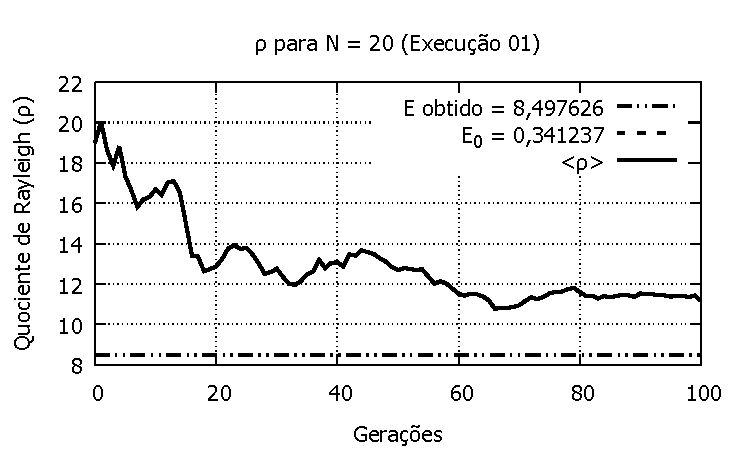
\includegraphics[width=.45\textwidth]{figs/resultados/fitnessGrad/N20_01_rho.pdf}   \\
		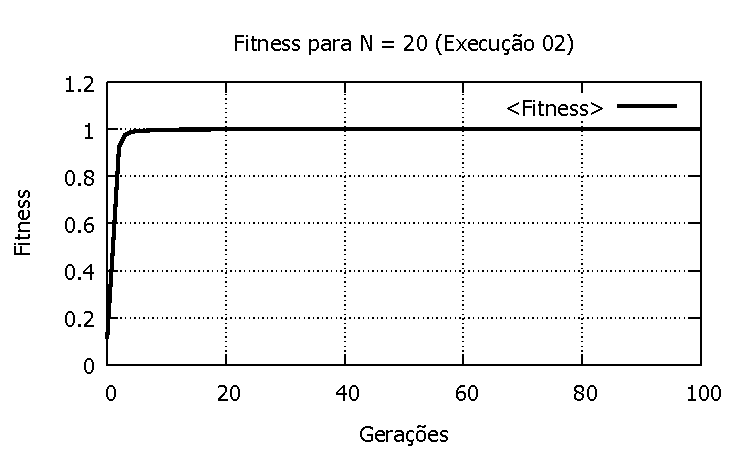
\includegraphics[width=.45\textwidth]{figs/resultados/fitnessGrad/N20_02_fitness.pdf} &
    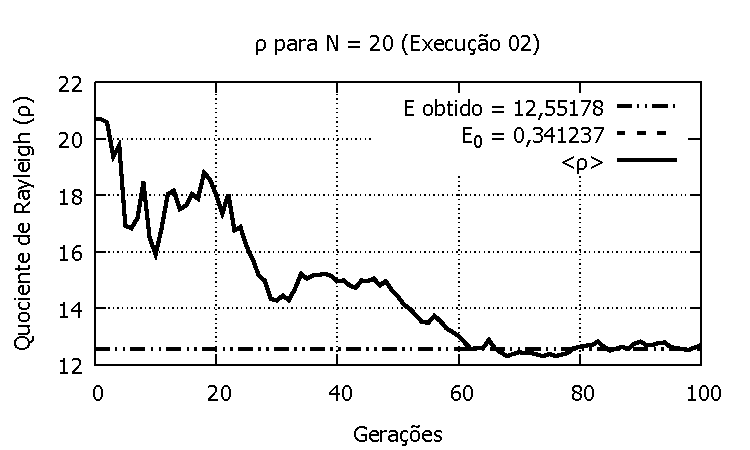
\includegraphics[width=.45\textwidth]{figs/resultados/fitnessGrad/N20_02_rho.pdf}   \\
		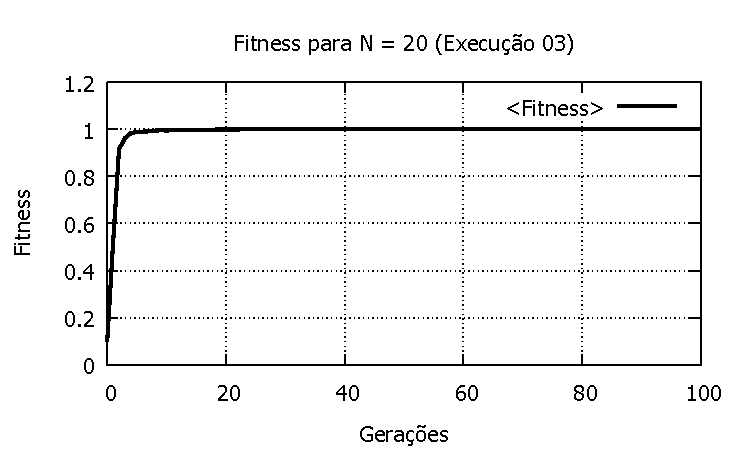
\includegraphics[width=.45\textwidth]{figs/resultados/fitnessGrad/N20_03_fitness.pdf} &
    \includegraphics[width=.45\textwidth]{figs/resultados/fitnessGrad/N20_03_rho.pdf}   \\
		\includegraphics[width=.45\textwidth]{figs/resultados/fitnessGrad/N20_04_fitness.pdf} &
    \includegraphics[width=.45\textwidth]{figs/resultados/fitnessGrad/N20_04_rho.pdf}   \\
		\includegraphics[width=.45\textwidth]{figs/resultados/fitnessGrad/N20_05_fitness.pdf} &
    \includegraphics[width=.45\textwidth]{figs/resultados/fitnessGrad/N20_05_rho.pdf}
    %\multicolumn{2}{c}{\includegraphics[width=.23\textwidth]{example-image-a}}
  \end{tabular}
  \caption{Execuções N = 20.}
	\label{fig:execucoes_N20}
\end{figure}

\begin{figure}[htbp]
\centering
  \begin{tabular}{@{}cc@{}}
    \includegraphics[width=.45\textwidth]{figs/resultados/fitnessGrad/N30_01_fitness.pdf} &
    \includegraphics[width=.45\textwidth]{figs/resultados/fitnessGrad/N30_01_rho.pdf}   \\
		\includegraphics[width=.45\textwidth]{figs/resultados/fitnessGrad/N30_02_fitness.pdf} &
    \includegraphics[width=.45\textwidth]{figs/resultados/fitnessGrad/N30_02_rho.pdf}   \\
		\includegraphics[width=.45\textwidth]{figs/resultados/fitnessGrad/N30_03_fitness.pdf} &
    \includegraphics[width=.45\textwidth]{figs/resultados/fitnessGrad/N30_03_rho.pdf}   \\
		\includegraphics[width=.45\textwidth]{figs/resultados/fitnessGrad/N30_04_fitness.pdf} &
    \includegraphics[width=.45\textwidth]{figs/resultados/fitnessGrad/N30_04_rho.pdf}   \\
		\includegraphics[width=.45\textwidth]{figs/resultados/fitnessGrad/N30_05_fitness.pdf} &
    \includegraphics[width=.45\textwidth]{figs/resultados/fitnessGrad/N30_05_rho.pdf}
    %\multicolumn{2}{c}{\includegraphics[width=.23\textwidth]{example-image-a}}
  \end{tabular}
  \caption{Execuções N = 30.}
	\label{fig:execucoes_N30}
\end{figure}

\begin{figure}[htbp]
\centering
  \begin{tabular}{@{}cc@{}}
    \includegraphics[width=.45\textwidth]{figs/resultados/fitnessGrad/N40_01_fitness.pdf} &
    \includegraphics[width=.45\textwidth]{figs/resultados/fitnessGrad/N40_01_rho.pdf}   \\
		\includegraphics[width=.45\textwidth]{figs/resultados/fitnessGrad/N40_02_fitness.pdf} &
    \includegraphics[width=.45\textwidth]{figs/resultados/fitnessGrad/N40_02_rho.pdf}   \\
		\includegraphics[width=.45\textwidth]{figs/resultados/fitnessGrad/N40_03_fitness.pdf} &
    \includegraphics[width=.45\textwidth]{figs/resultados/fitnessGrad/N40_03_rho.pdf}   \\
		\includegraphics[width=.45\textwidth]{figs/resultados/fitnessGrad/N40_04_fitness.pdf} &
    \includegraphics[width=.45\textwidth]{figs/resultados/fitnessGrad/N40_04_rho.pdf}   \\
		\includegraphics[width=.45\textwidth]{figs/resultados/fitnessGrad/N40_05_fitness.pdf} &
    \includegraphics[width=.45\textwidth]{figs/resultados/fitnessGrad/N40_05_rho.pdf}
    %\multicolumn{2}{c}{\includegraphics[width=.23\textwidth]{example-image-a}}
  \end{tabular}
  \caption{Execuções N = 40.}
	\label{fig:execucoes_N40}
\end{figure}
%\chapter{Execuções para o \textit{fitness} $f_i = e^{-\lambda(\rho_i - E_L)^2}$}

\begin{figure}[phtb]
	\centering
  \begin{tabular}{@{}cc@{}}
    \includegraphics[width=.40\textwidth]{figs/resultados/fitnessEL/N-10_E-0_fitness-extendido.pdf} &
    \includegraphics[width=.40\textwidth]{figs/resultados/fitnessEL/N-10_E-0_rho_extendido.pdf}   \\
		\includegraphics[width=.40\textwidth]{figs/resultados/fitnessEL/N-10_E-1_fitness-extendido.pdf} &
    \includegraphics[width=.40\textwidth]{figs/resultados/fitnessEL/N-10_E-1_rho_extendido.pdf}   \\
		\includegraphics[width=.40\textwidth]{figs/resultados/fitnessEL/N-10_E-2_fitness-extendido.pdf} &
    \includegraphics[width=.40\textwidth]{figs/resultados/fitnessEL/N-10_E-2_rho_extendido.pdf}   \\
		\includegraphics[width=.40\textwidth]{figs/resultados/fitnessEL/N-10_E-3_fitness-extendido.pdf} &
    \includegraphics[width=.40\textwidth]{figs/resultados/fitnessEL/N-10_E-3_rho_extendido.pdf}   \\
		\includegraphics[width=.40\textwidth]{figs/resultados/fitnessEL/N-10_E-4_fitness-extendido.pdf} &
    \includegraphics[width=.40\textwidth]{figs/resultados/fitnessEL/N-10_E-4_rho_extendido.pdf} \\
		\includegraphics[width=.40\textwidth]{figs/resultados/fitnessEL/N-10_E-5_fitness-extendido.pdf} &
    \includegraphics[width=.40\textwidth]{figs/resultados/fitnessEL/N-10_E-5_rho_extendido.pdf}
  \end{tabular}
  \caption{Execuções para N = 10 com o \textit{fitness} $f_i = e^{-\lambda(\rho_i - E_L)^2}$.}
	\label{fig:execucoes_N10_EL}
	\end{figure}
	
	\begin{figure}[phtb]
	\centering
  \begin{tabular}{@{}cc@{}}
		\includegraphics[width=.40\textwidth]{figs/resultados/fitnessEL/N-20_E-1_fitness-extendido.pdf} &
    \includegraphics[width=.40\textwidth]{figs/resultados/fitnessEL/N-20_E-1_rho_extendido.pdf}   \\
		\includegraphics[width=.40\textwidth]{figs/resultados/fitnessEL/N-20_E-2_fitness-extendido.pdf} &
    \includegraphics[width=.40\textwidth]{figs/resultados/fitnessEL/N-20_E-2_rho_extendido.pdf}   \\
		\includegraphics[width=.40\textwidth]{figs/resultados/fitnessEL/N-20_E-3_fitness-extendido.pdf} &
    \includegraphics[width=.40\textwidth]{figs/resultados/fitnessEL/N-20_E-3_rho_extendido.pdf}   \\
		\includegraphics[width=.40\textwidth]{figs/resultados/fitnessEL/N-20_E-4_fitness-extendido.pdf} &
    \includegraphics[width=.40\textwidth]{figs/resultados/fitnessEL/N-20_E-4_rho_extendido.pdf} \\
		\includegraphics[width=.40\textwidth]{figs/resultados/fitnessEL/N-20_E-5_fitness-extendido.pdf} &
    \includegraphics[width=.40\textwidth]{figs/resultados/fitnessEL/N-20_E-5_rho_extendido.pdf}
  \end{tabular}
  \caption{Execuções para N = 20 com o \textit{fitness} $f_i = e^{-\lambda(\rho_i - E_L)^2}$.}
	\label{fig:execucoes_N20_EL}
	\end{figure}
	
	\begin{figure}[phtb]
	\centering
  \begin{tabular}{@{}cc@{}}
		\includegraphics[width=.40\textwidth]{figs/resultados/fitnessEL/N-30_E-1_fitness-extendido.pdf} &
    \includegraphics[width=.40\textwidth]{figs/resultados/fitnessEL/N-30_E-1_rho_extendido.pdf}   \\
		\includegraphics[width=.40\textwidth]{figs/resultados/fitnessEL/N-30_E-2_fitness-extendido.pdf} &
    \includegraphics[width=.40\textwidth]{figs/resultados/fitnessEL/N-30_E-2_rho_extendido.pdf}   \\
		\includegraphics[width=.40\textwidth]{figs/resultados/fitnessEL/N-30_E-3_fitness-extendido.pdf} &
    \includegraphics[width=.40\textwidth]{figs/resultados/fitnessEL/N-30_E-3_rho_extendido.pdf}   \\
		\includegraphics[width=.40\textwidth]{figs/resultados/fitnessEL/N-30_E-4_fitness-extendido.pdf} &
    \includegraphics[width=.40\textwidth]{figs/resultados/fitnessEL/N-30_E-4_rho_extendido.pdf} \\
		\includegraphics[width=.40\textwidth]{figs/resultados/fitnessEL/N-30_E-5_fitness-extendido.pdf} &
    \includegraphics[width=.40\textwidth]{figs/resultados/fitnessEL/N-30_E-5_rho_extendido.pdf}
  \end{tabular}
  \caption{Execuções para N = 30 com o \textit{fitness} $f_i = e^{-\lambda(\rho_i - E_L)^2}$.}
	\label{fig:execucoes_N30_EL}
	\end{figure}
	
	\begin{figure}[phtb]
	\centering
  \begin{tabular}{@{}cc@{}}
		\includegraphics[width=.40\textwidth]{figs/resultados/fitnessEL/N-40_E-1_fitness-extendido.pdf} &
    \includegraphics[width=.40\textwidth]{figs/resultados/fitnessEL/N-40_E-1_rho_extendido.pdf}   \\
		\includegraphics[width=.40\textwidth]{figs/resultados/fitnessEL/N-40_E-2_fitness-extendido.pdf} &
    \includegraphics[width=.40\textwidth]{figs/resultados/fitnessEL/N-40_E-2_rho_extendido.pdf}   \\
		\includegraphics[width=.40\textwidth]{figs/resultados/fitnessEL/N-40_E-3_fitness-extendido.pdf} &
    \includegraphics[width=.40\textwidth]{figs/resultados/fitnessEL/N-40_E-3_rho_extendido.pdf}   \\
		\includegraphics[width=.40\textwidth]{figs/resultados/fitnessEL/N-40_E-4_fitness-extendido.pdf} &
    \includegraphics[width=.40\textwidth]{figs/resultados/fitnessEL/N-40_E-4_rho_extendido.pdf}		\\
		\includegraphics[width=.40\textwidth]{figs/resultados/fitnessEL/N-40_E-5_fitness-extendido.pdf} &
    \includegraphics[width=.40\textwidth]{figs/resultados/fitnessEL/N-40_E-5_rho_extendido.pdf}
  \end{tabular}
  \caption{Execuções para N = 40 com o \textit{fitness} $f_i = e^{-\lambda(\rho_i - E_L)^2}$.}
	\label{fig:execucoes_N40_EL}
	\end{figure}
%\chapter{Execuções para a variação de $E_L$ em torno de $E_0$}

\begin{figure}[phtb]
	\centering
  \begin{tabular}{@{}cc@{}}
    \includegraphics[width=.40\textwidth]{figs/resultados/fitnessEL/N-10_E-0_fitness-extendido.pdf} &
    \includegraphics[width=.40\textwidth]{figs/resultados/fitnessEL/N-10_E-0_rho_extendido.pdf}   \\
		\includegraphics[width=.40\textwidth]{figs/resultados/fitnessEL/N-10_E-1_fitness-extendido.pdf} &
    \includegraphics[width=.40\textwidth]{figs/resultados/fitnessEL/N-10_E-1_rho_extendido.pdf}   \\
		\includegraphics[width=.40\textwidth]{figs/resultados/fitnessEL/N-10_E-2_fitness-extendido.pdf} &
    \includegraphics[width=.40\textwidth]{figs/resultados/fitnessEL/N-10_E-2_rho_extendido.pdf}   \\
		\includegraphics[width=.40\textwidth]{figs/resultados/fitnessEL/N-10_E-3_fitness-extendido.pdf} &
    \includegraphics[width=.40\textwidth]{figs/resultados/fitnessEL/N-10_E-3_rho_extendido.pdf}   \\
		\includegraphics[width=.40\textwidth]{figs/resultados/fitnessEL/N-10_E-4_fitness-extendido.pdf} &
    \includegraphics[width=.40\textwidth]{figs/resultados/fitnessEL/N-10_E-4_rho_extendido.pdf} \\
		\includegraphics[width=.40\textwidth]{figs/resultados/fitnessEL/N-10_E-5_fitness-extendido.pdf} &
    \includegraphics[width=.40\textwidth]{figs/resultados/fitnessEL/N-10_E-5_rho_extendido.pdf}
  \end{tabular}
  \caption{Execuções para N = 10 com o \textit{fitness} $f_i = e^{-\lambda(\rho_i - E_L)^2}$.}
	\label{fig:execucoes_N10_EL}
	\end{figure}
	
	\begin{figure}[phtb]
	\centering
  \begin{tabular}{@{}cc@{}}
		\includegraphics[width=.40\textwidth]{figs/resultados/fitnessEL/N-20_E-1_fitness-extendido.pdf} &
    \includegraphics[width=.40\textwidth]{figs/resultados/fitnessEL/N-20_E-1_rho_extendido.pdf}   \\
		\includegraphics[width=.40\textwidth]{figs/resultados/fitnessEL/N-20_E-2_fitness-extendido.pdf} &
    \includegraphics[width=.40\textwidth]{figs/resultados/fitnessEL/N-20_E-2_rho_extendido.pdf}   \\
		\includegraphics[width=.40\textwidth]{figs/resultados/fitnessEL/N-20_E-3_fitness-extendido.pdf} &
    \includegraphics[width=.40\textwidth]{figs/resultados/fitnessEL/N-20_E-3_rho_extendido.pdf}   \\
		\includegraphics[width=.40\textwidth]{figs/resultados/fitnessEL/N-20_E-4_fitness-extendido.pdf} &
    \includegraphics[width=.40\textwidth]{figs/resultados/fitnessEL/N-20_E-4_rho_extendido.pdf} \\
		\includegraphics[width=.40\textwidth]{figs/resultados/fitnessEL/N-20_E-5_fitness-extendido.pdf} &
    \includegraphics[width=.40\textwidth]{figs/resultados/fitnessEL/N-20_E-5_rho_extendido.pdf}
  \end{tabular}
  \caption{Execuções para N = 20 com o \textit{fitness} $f_i = e^{-\lambda(\rho_i - E_L)^2}$.}
	\label{fig:execucoes_N20_EL}
	\end{figure}
	
	\begin{figure}[phtb]
	\centering
  \begin{tabular}{@{}cc@{}}
		\includegraphics[width=.40\textwidth]{figs/resultados/fitnessEL/N-30_E-1_fitness-extendido.pdf} &
    \includegraphics[width=.40\textwidth]{figs/resultados/fitnessEL/N-30_E-1_rho_extendido.pdf}   \\
		\includegraphics[width=.40\textwidth]{figs/resultados/fitnessEL/N-30_E-2_fitness-extendido.pdf} &
    \includegraphics[width=.40\textwidth]{figs/resultados/fitnessEL/N-30_E-2_rho_extendido.pdf}   \\
		\includegraphics[width=.40\textwidth]{figs/resultados/fitnessEL/N-30_E-3_fitness-extendido.pdf} &
    \includegraphics[width=.40\textwidth]{figs/resultados/fitnessEL/N-30_E-3_rho_extendido.pdf}   \\
		\includegraphics[width=.40\textwidth]{figs/resultados/fitnessEL/N-30_E-4_fitness-extendido.pdf} &
    \includegraphics[width=.40\textwidth]{figs/resultados/fitnessEL/N-30_E-4_rho_extendido.pdf} \\
		\includegraphics[width=.40\textwidth]{figs/resultados/fitnessEL/N-30_E-5_fitness-extendido.pdf} &
    \includegraphics[width=.40\textwidth]{figs/resultados/fitnessEL/N-30_E-5_rho_extendido.pdf}
  \end{tabular}
  \caption{Execuções para N = 30 com o \textit{fitness} $f_i = e^{-\lambda(\rho_i - E_L)^2}$.}
	\label{fig:execucoes_N30_EL}
	\end{figure}
	
	\begin{figure}[phtb]
	\centering
  \begin{tabular}{@{}cc@{}}
		\includegraphics[width=.40\textwidth]{figs/resultados/fitnessEL/N-40_E-1_fitness-extendido.pdf} &
    \includegraphics[width=.40\textwidth]{figs/resultados/fitnessEL/N-40_E-1_rho_extendido.pdf}   \\
		\includegraphics[width=.40\textwidth]{figs/resultados/fitnessEL/N-40_E-2_fitness-extendido.pdf} &
    \includegraphics[width=.40\textwidth]{figs/resultados/fitnessEL/N-40_E-2_rho_extendido.pdf}   \\
		\includegraphics[width=.40\textwidth]{figs/resultados/fitnessEL/N-40_E-3_fitness-extendido.pdf} &
    \includegraphics[width=.40\textwidth]{figs/resultados/fitnessEL/N-40_E-3_rho_extendido.pdf}   \\
		\includegraphics[width=.40\textwidth]{figs/resultados/fitnessEL/N-40_E-4_fitness-extendido.pdf} &
    \includegraphics[width=.40\textwidth]{figs/resultados/fitnessEL/N-40_E-4_rho_extendido.pdf}		\\
		\includegraphics[width=.40\textwidth]{figs/resultados/fitnessEL/N-40_E-5_fitness-extendido.pdf} &
    \includegraphics[width=.40\textwidth]{figs/resultados/fitnessEL/N-40_E-5_rho_extendido.pdf}
  \end{tabular}
  \caption{Execuções para N = 40 com o \textit{fitness} $f_i = e^{-\lambda(\rho_i - E_L)^2}$.}
	\label{fig:execucoes_N40_EL}
	\end{figure}
%\chapter{Formato matricial da Equação de Schrödinger independente do tempo}

Página 36 do \cite{Cohen1}.

-------------------------------

Equação de Schrödinger com potencial dependente do tempo:
	
	\begin{equation}
		i\hbar\frac{\partial}{\partial t} \psi(\textbf{r},t) =  - \frac{\hbar^2}{2m}\Delta\psi(\textbf{r},t) + V(\textbf{r},t)\psi(\textbf{r},t),
	\end{equation}
	onde $\Delta$ é o operador Laplaciano $\partial / \partial x^2 + \partial / \partial y^2 + \partial / \partial z^2$.
	
	
	Equação de Schrödinger com potencial independente do tempo:
	
	\begin{equation}\label{eq:SchrodingerIndTempo}
		i\hbar\frac{\partial}{\partial t} \psi(\textbf{r},t) =  - \frac{\hbar^2}{2m}\Delta\psi(\textbf{r},t) + V(\textbf{r})\psi(\textbf{r},t)
	\end{equation}
	
	Existe soluções na forma
	
	\begin{equation}
		\psi(\textbf{r},t) = \phi(\textbf{r})\chi(t)
	\end{equation}
	
	A função 
	
	\begin{equation}\label{eq:solucaoSchro}
		\psi(\textbf{r},t) = \phi(\textbf{r})\mbox{e}^{-i \omega t}
	\end{equation}
	é uma solução da equação \ref{eq:SchrodingerIndTempo}, chamada de Solução Estacionária da Equação de Schrödinger. Ela leva a uma densidade de probabilidade $|\psi(\textbf{r},t)|^2 = |\phi(\textbf{r})|^2$ independente do tempo. Dizemos que as variáveis de espaço e tempo foram separadas.
	
	A função $\phi(\textbf{r})$ deve satisfazer a equação
	
	\begin{equation}\label{eq:SchroNoR}
		- \frac{\hbar^2}{2m} \Delta \phi(\textbf{r}) + V(\textbf{r}) \phi(\textbf{r}) = \hbar \omega \phi(\textbf{r})
	\end{equation}
	
	A equação \ref{eq:SchroNoR} pode ser reescrita como
	
	\begin{equation}\label{eq:SchroNoRReescrita}
			\left[-\frac{\hbar^2}{2m}\Delta + V(\textbf{r})\right] \phi(\textbf{r}) = \hbar \omega \phi(\textbf{r})
	\end{equation}
	
	Definindo 
	
	\begin{equation}
	H  = -\frac{\hbar^2}{2m}\Delta + V(\textbf{r}),
	\end{equation}
	a equação \ref{eq:SchroNoRReescrita} fica
	
	\begin{equation}\label{eq:H_com_hw}
		H\phi(\textbf{r}) = \hbar \omega \phi(\textbf{r})
	\end{equation}
	
	De acordo com as relações de Planck-Einstein, um estado estacionário é um estado com energia bem definida e com valor $E = \hbar \omega$ ($\omega = 2 \pi \nu$). Finalmente, a equação \ref{eq:H_com_hw} fica
	
	\begin{equation}\label{eq:Schro_Indepentende_do_Tempo}
		H\phi(\textbf{r}) = E \phi(\textbf{r}).
	\end{equation}
	
	A equação \ref{eq:Schro_Indepentende_do_Tempo} é, então, uma equação de autovalores para o operador linear $H$: a aplicação de $H$ à autofunção $\phi(\textbf{r})$ leva à mesma função, multiplicada pelo autovalor correspondente $E$. As energias permitidas são, portanto, os autovalores do operador $H$. Está associada à origem da quantização da energia.
	
	

\end{apendicesenv}

% ---- Anexos ----
%\begin{anexosenv}
% Imprime uma página indicando o início dos anexos
%\partanexos

%\include{anexoA}
%\include{anexoB}

%\end{anexosenv}

% ---- INDICE REMISSIVO ----
%\printindex

\end{document} 